\documentclass[11pt,twoside]{report}

%%%%%%%%%%%%%%%%%%%%%%%%%%%%%%%%%%%%%%%%%%%%%%%%%%%%%%%%%%%%%%%%%%%%%%%%%%%%%

% Definitions for the title page
% Edit these to provide the correct information
% e.g. \newcommand{\reportauthor}{Timothy Kimber}

\newcommand{\reporttitle}{Java Algorithms for Computer Performance Analysis}
\newcommand{\reportauthor}{Ong Wai Hong}
\newcommand{\supervisor}{Dr. Giuliano Casale}
\newcommand{\secondmarker}{Prof. Peter G. Harrison}
\newcommand{\degreetype}{Computing Science}

%%%%%%%%%%%%%%%%%%%%%%%%%%%%%%%%%%%%%%%%%%%%%%%%%%%%%%%%%%%%%%%%%%%%%%%%%%%%%

% load some definitions and default packages
%%%%%%%%%%%%%%%%%%%%%%%%%%%%%%%%%%%%%%%%%
% University Assignment Title Page 
% LaTeX Template
% Version 1.0 (27/12/12)
%
% This template has been downloaded from:
% http://www.LaTeXTemplates.com
%
% Original author:
% WikiBooks (http://en.wikibooks.org/wiki/LaTeX/Title_Creation)
%
% License:
% CC BY-NC-SA 3.0 (http://creativecommons.org/licenses/by-nc-sa/3.0/)
% 
%
%%%%%%%%%%%%%%%%%%%%%%%%%%%%%%%%%%%%%%%%%
%----------------------------------------------------------------------------------------
%	PACKAGES AND OTHER DOCUMENT CONFIGURATIONS
%----------------------------------------------------------------------------------------
\usepackage[a4paper,hmargin=2.8cm,vmargin=2.0cm,includeheadfoot]{geometry}
\usepackage{textpos}
\usepackage{natbib} % for bibliography
\usepackage{tabularx,longtable,multirow,subfigure,caption}%hangcaption
\usepackage{fncylab} %formatting of labels
\usepackage{fancyhdr} % page layout
\usepackage{url} % URLs
\usepackage[english]{babel}
\usepackage{amsmath}
\usepackage{graphicx}
\usepackage{dsfont}
\usepackage{epstopdf} % automatically replace .eps with .pdf in graphics
\usepackage{backref} % needed for citations
\usepackage{array}
\usepackage{latexsym}
\usepackage[toc,page]{appendix}
\usepackage[pdftex,pagebackref,hypertexnames=false,colorlinks]{hyperref} % provide links in pdf

\hypersetup{pdftitle={},
  pdfsubject={}, 
  pdfauthor={},
  pdfkeywords={}, 
  pdfstartview=FitH,
  pdfpagemode={UseOutlines},% None, FullScreen, UseOutlines
  bookmarksnumbered=true, bookmarksopen=true, colorlinks,
    citecolor=black,%
    filecolor=black,%
    linkcolor=black,%
    urlcolor=black}

\usepackage[all]{hypcap}

\usepackage{amsthm}
%\usepackage{color}
%\usepackage[tight,ugly]{units}
%\usepackage{float}
\usepackage{empheq}
\usepackage[most]{tcolorbox}
%\usepackage[colorinlistoftodos]{todonotes}
%\usepackage{ntheorem}
% \theoremstyle{break}
\newtheorem{theorem}{Theorem}[section]
\newtheorem{corollary}{Corollary}[theorem]
\newtheorem{lemma}[theorem]{Lemma}
% \newtheorem{remark}{Remark}
%\newtheorem{proof}{Proof}
\newtheorem{definition}{Definition}[section]
\usepackage{amssymb} % for special math symbols
\usepackage{booktabs} % for special tables
\usepackage{float} % for fixed tables/figures
\usepackage{enumitem}
\usepackage{listings}
\usepackage{color}

%%% Default fonts
\renewcommand*{\rmdefault}{bch}
\renewcommand*{\ttdefault}{cmtt}



%%% Default settings (page layout)
\setlength{\parindent}{0em}  % indentation of paragraph

\setlength{\headheight}{14.5pt}
\pagestyle{fancy}
\renewcommand{\chaptermark}[1]{\markboth{\chaptername\ \thechapter.\ #1}{}} 

\fancyfoot[ER,OL]{\sffamily\textbf{\thepage}}%Page no. in the left on odd pages and on right on even pages
\fancyfoot[OC,EC]{\sffamily }
\renewcommand{\headrulewidth}{0.1pt}
\renewcommand{\footrulewidth}{0.1pt}
\captionsetup{margin=10pt,font=small,labelfont=bf}

%--- chapter heading

\def\@makechapterhead#1{%
  \vspace*{10\p@}%
  {\parindent \z@ \raggedright \sffamily
    \interlinepenalty\@M
    \Huge\bfseries \thechapter \space\space #1\par\nobreak
    \vskip 30\p@
  }}

%---chapter heading for \chapter*  
\def\@makeschapterhead#1{%
  \vspace*{10\p@}%
  {\parindent \z@ \raggedright
    \sffamily
    \interlinepenalty\@M
    \Huge \bfseries  #1\par\nobreak
    \vskip 30\p@
  }}
  
% -- Java code listing

\definecolor{dkgreen}{rgb}{0,0.6,0}
\definecolor{gray}{rgb}{0.5,0.5,0.5}
\definecolor{mauve}{rgb}{0.58,0,0.82}

\lstset{frame=tb,
  language=Java,
  aboveskip=3mm,
  belowskip=3mm,
  showstringspaces=false,
  columns=flexible,
  basicstyle={\small\ttfamily},
  numbers=none,
  numberstyle=\tiny\color{gray},
  keywordstyle=\color{blue},
  commentstyle=\color{dkgreen},
  stringstyle=\color{mauve},
  breaklines=true,
  breakatwhitespace=true,
  tabsize=3
}

% --- pretty math box

\newtcbox{\mymath}[1][]{%
    nobeforeafter, math upper, tcbox raise base,
    enhanced, colframe=gray,
    colback=blue!60!green!10, boxrule=1pt,
    #1}

\newtcbox{\mymathtwo}[1][]{%
    nobeforeafter, math upper, tcbox raise base,
    enhanced, colframe=black,
    colback=white, boxrule=.5pt,
    #1}

\allowdisplaybreaks

% load some macros
% Here, you can define your own macros. Some examples are given below.

\newcommand{\R}[0]{\mathds{R}} % real numbers
\newcommand{\Z}[0]{\mathds{Z}} % integers
\newcommand{\N}[0]{\mathds{N}} % natural numbers
\newcommand{\C}[0]{\mathds{C}} % complex numbers
\renewcommand{\vec}[1]{{\boldsymbol{{#1}}}} % vector
\newcommand{\mat}[1]{{\boldsymbol{{#1}}}} % matrix


\date{September 2018}

\begin{document}

% load title page
% Last modification: 2015-08-17 (Marc Deisenroth)
\begin{titlepage}

\newcommand{\HRule}{\rule{\linewidth}{0.5mm}} % Defines a new command for the horizontal lines, change thickness here


%----------------------------------------------------------------------------------------
%	LOGO SECTION
%----------------------------------------------------------------------------------------


\includegraphics[width = 4cm]{./figures/imperial}\\[0.5cm] 

\center % Center remainder of the page

%----------------------------------------------------------------------------------------
%	HEADING SECTIONS
%----------------------------------------------------------------------------------------

\textsc{\Large Imperial College London}\\[0.5cm] 
\textsc{\large Department of Computing}\\[0.5cm] 

%----------------------------------------------------------------------------------------
%	TITLE SECTION
%----------------------------------------------------------------------------------------

\HRule \\[0.4cm]
{ \huge \bfseries \reporttitle}\\ % Title of your document
\HRule \\[1.5cm]
 
%----------------------------------------------------------------------------------------
%	AUTHOR SECTION
%----------------------------------------------------------------------------------------

\begin{minipage}{0.4\textwidth}
\begin{flushleft} \large
\emph{Author:}\\
\reportauthor % Your name
\end{flushleft}
\end{minipage}
~
\begin{minipage}{0.4\textwidth}
\begin{flushright} \large
\emph{Supervisor:} \\
\supervisor % Supervisor's Name
\end{flushright}
\end{minipage}\\[4cm]


%----------------------------------------------------------------------------------------
%	FOOTER & DATE SECTION
%----------------------------------------------------------------------------------------
\vfill % Fill the rest of the page with whitespace
Submitted in partial fulfillment of the requirements for the MSc degree in
\degreetype~of Imperial College London\\[0.5cm]

\makeatletter
\@date 
\makeatother


\end{titlepage}



% page numbering etc.
\pagenumbering{roman}
\clearpage{\pagestyle{empty}\cleardoublepage}
\setcounter{page}{1}
\pagestyle{fancy}

%%%%%%%%%%%%%%%%%%%%%%%%%%%%%%%%%%%%
\begin{abstract}
    Queueing network theory is an important probabilistic analytical modelling tool for computer performance analysis, when designing and optimizing computer systems. A number of exact methods exist for the calculation of performance measures and state probability normalizing constants. The latter quantity is important as it appears in likelihood functions for the inference of queueing network models based on measurement data. These exact algorithms include the Convolution algorithm, RECAL, and MoM algorithms. While these provide exact answers, they generally do not scale well with the number of stations, customer classes and customer populations in the model.
    \\\\
    A new integral form of the normalizing constant, which takes the form of an integral on the simplex is proposed. Through the logistic (or log-ratio) transform, Laplace's method could be applied to compute this quantity. Laplace's method's applicability to this problem indicates the suitability of Importance Sampling on the integration domain, centered around the integrand's stationary point.
    \\\\
    This project focuses on the implementation of the Logistic Sampling algorithm as it was initially proposed, in Java. This involved a thorough understanding of the proofs and methods that make this computation possible. Novel contributions to this project include several new results concerning different transform types. Besides that, this project was able to see the derivation of results for, and implementation of an extended Logistic Sampling algorithm that catered for multi-server models.
\end{abstract}

\cleardoublepage
%%%%%%%%%%%%%%%%%%%%%%%%%%%%%%%%%%%%
\section*{Acknowledgments}
I wish to thank my supervisor, Dr. Giuliano Casale for his patience and enthusiasm in guiding me through this project.
\\\\
I also wish to thank my family for their financial and emotional support throughout this course

\clearpage{\pagestyle{empty}\cleardoublepage}

%%%%%%%%%%%%%%%%%%%%%%%%%%%%%%%%%%%%
%--- table of contents
\fancyhead[RE,LO]{\sffamily {Table of Contents}}
\tableofcontents 


\clearpage{\pagestyle{empty}\cleardoublepage}
\pagenumbering{arabic}
\setcounter{page}{1}
\fancyhead[LE,RO]{Sec. \thesection}
\fancyhead[LO,RE]{\slshape \leftmark}

%%%%%%%%%%%%%%%%%%%%%%%%%%%%%%%%%%%%
\chapter{Introduction}

\begin{figure}[tb]
\centering

\includegraphics[width = 0.4\hsize]{./figures/imperial}
\caption{Imperial College Logo. It's nice blue, and the font is quite stylish. But you can choose a different one if you don't like it.}
\label{fig:logo}
\end{figure}

Figure~\ref{fig:logo} is an example of a figure. 

%%%%%%%%%%%%%%%%%%%%%%%%%%%%%%%%%%%%
\chapter{Background}

The aim of this chapter is to provide a theoretical background to the reader based on the ideas behind queueing theory, which forms the basis of the work done in this project. Besides that it also aims to provide context regarding the specific problems this project wishes to address with respect to queueing networks and its properties of interest.
\\\\
The summary of this chapter is as follows: section \ref{sec:intro_to_markov} aims to provide important definitions and the basic mathematical theory of Markov chains which underlies the field of queueing theory and queueing networks. Sections \ref{sec:QueueingSystems} and \ref{sec:QNetworks} introduce the idea of service centres, queues, and queueing networks, focusing on Markovian queues which are of primary interest in this project. Finally, section \ref{sec:AlgorithmsPFQN} introduces what is called the product-form solution of queueing networks, which is an important result that enables the formulation of efficient algorithms for the analysis and evaluation of queueing networks.

\section{Introduction to Markov Chains}\label{sec:intro_to_markov}

In this section we provide the definitions necessary to define Markov Processes, and Markov Chains, with special attention paid to Continuous-Time Markov Chains (CTMC's). This section assumes knowledge of stochastic processes.

\begin{definition}
    % Def 2.3
    A stochastic process \(\{X_t : t \in T\}\) constitutes a Markov process, if \(\forall t = t_0 < t_1 < ... < t_n\) and all \(s_i \in S\) it satisfies the Markov property:
    \begin{equation}\label{eq:MarkovProperty}
        P(X_{t_{n+1}}=s_{n+1} | X_{t_n} = s_n, X_{t_{n-1}}=s_{n-1}, ... , X_{t_0}=s_0) = P(X_{t_{n+1}}=s_{n+1} | X_{t_n} = s_n)
    \end{equation}
\end{definition}

The Markov property essentially states that the conditional PDF of \(X_{t_{n+1}}\) depends only on the last previous value of \(X_{t_n}\) and not not the earlier values before \(X_{t_n}\). 
\\\\
The concept of time-homogeneity is stated as the following:

\begin{definition}
    A Markov process is time-homogeneous if the following holds for the PDF of a random variable of a stochastic process at time \(t\), \(X_{t}\):
    \begin{equation}\label{eq:TimeHomogeneity}
        P(X_{t + \tau}=s_{i} | X_{t}=s_{j}) = P(X_{\tau}=s_{i} | X_{0}=s_{j})
    \end{equation}
\end{definition}

This property essentially states that the conditional PDF of \(X_{t+\tau}=s_{i}\) on the states given the state at \(X_{t}=s_{j}\) does not depend on the value of the time instant \(t\), but only on the elapsed time \(\tau\). Time homogeneity implies the memoryless property for state holding times, or state sojourn times.

\begin{definition}
    A discrete time Markov chain (DTMC) governs a discrete time (as opposed to continuous time) stochastic process, if the process has a countable state space \(S\), and satisfies the following relations on the conditional PMF, given \(n+1\) consecutive discrete time points of observation:
    \[P(X_{n+1} | X_n=s_n , X_{n-1}=s_{n-1} , ... , X_0=s_0 ) = P(X_{n+1} | X_n=s_n)\]
    This is Markov property re-stated in discrete time, for a discrete state space. 
\end{definition}

A DTMC is characterized by the state transition matrix \(\mathbf{P}\), where \(p_{ij}\) is the state transition matrix, giving a probability to transition from state \(s_i\) to state \(s_j\) at the next time instant, given that the current state of the discrete-time Markov process is \(s_j\). A time-homogeneous DTMC has a fixed state transition matrix.
\\\\
Several other desirable properties for a DTMC to have include \textit{irreducibility}, consisting only of \textit{positive recurrent states}, and is \textit{aperiodic}. The reader is advised to consult \cite{Bolch2006QueueingApplications} for details. The above properties all belong to what is called an \textit{ergodic} DTMC, and implies that a unique steady-state probability vector \(\mathbf{\pi}\) for the DTMC exists. This is given by the solution to the equation:
\begin{equation}
    \boldsymbol{\pi} = \mathbf{P}\boldsymbol{\pi}
\end{equation}

\begin{definition}
    A Continuous time Markov Chain (CTMC) governs a stochastic process, if the stochastic process satisfies the Markov property (\ref{eq:MarkovProperty}) for a countable state space \(S\). It is time homogeneous if it satisfies (\ref{eq:TimeHomogeneity}). 
\end{definition}
Given state transition probabilities \(p_{ij}(u,v)\) between times \(u\) and \(v\), and the unconditional state probabilities \(p_i(u)\), \(p_j(v)\). The following equation holds by the law of total probability:
\begin{equation}
    p_j(v) = \sum_{i \in S} p_{ij}(u,v) p_i(u)
\end{equation}
In the time-homogeneous case, this becomes:
\begin{equation}\label{eq:time_homo_unconditional_probs}
    p_j(t) = \sum_{i \in S} p_{ij}(0,t) p_i(0)
\end{equation}

The \textit{Chapman-Kolmogorov} equations are given, for a CTMC:
\begin{equation}\label{eq:CK_eqns}
    p_{ij}(u,v) = \sum_{k \in S} p_{ik}(u,w)p_{kj}(w,v)
\end{equation}
We can also define instantaneous transition rates \(q_{ij}(t)\) of a CTMC, and this is defined:
\begin{equation}\label{eq:transition_rates}
\begin{split}
    q_{ij}(t) & = \lim_{\Delta t \rightarrow 0} \frac{p_{ij}(t,t + \Delta t)}{\Delta t}, \quad i \neq j \\
    q_{ii}(t) & = \lim_{\Delta t \rightarrow 0} \frac{p_{ii}(t,t + \Delta t) - 1}{\Delta t} = -\sum_{j \neq i} q_{ij}(t)
\end{split}
\end{equation}

Without going into too much detailed derivations, the equations (\ref{eq:CK_eqns}) and (\ref{eq:transition_rates}) gives us the time-homogeneous version of the Kolmogorov forward equations:
\begin{equation}
    \frac{d p_{ij}(t)}{dt}  = \sum_{k \in S} p_{ik}(t)q_{kj}
\end{equation}
Where the time-independent transition rates \(q_{kj}\) is used. Combining this with (\ref{eq:time_homo_unconditional_probs}) gives us :
\begin{equation}
    \frac{d p_j (t)}{dt} = \sum_{i \in S} q_{ij} p_i(t)
\end{equation}

The time-homogeneity property and memorylessness property implies that the state holding time for a state \(s_i\) in a CTMC is exponentially distributed, and that the the probability of a transition \(p_{ij}\) in any given time interval \(\Delta t\) is Poisson-distributed:
\[p_{ij}(N=n) = \frac{(r \Delta t)^n exp(-r \Delta t)}{n!}\]

For an \textit{ergodic} CTMC, the steady-state distribution of \(p_j\) exists. By setting \(\frac{dp_i(t)}{dt} = 0\), this gives us what is known as the global balance equations:
\begin{equation}\label{eq:global_balance_equations}
  -p_i(t) \sum _ {j \in S, j \neq i}q_{ij} + \sum_{j\in S, j \neq i} p_j(t)q_{ji} = 0  
\end{equation}

Or in matrix form:
\[\mathbf{pQ=0}\]
Where \(\mathbf{Q}\) is a matrix where the off-diagonals elements are the inter-state transition rates, \(q_{ij}\), and the diagonal elements is the negative sum of the entire row: \(q_{ii} = -\sum _ {j \in S, j \neq i}q_{ij}\). In order to solve for \(\mathbf{p}\), one must introduce the normalizing condition \(\sum_i p_i = 1\) into the GBE's, so that \(\mathbf{Q}\) becomes non-singular.
\\\\
CTMC's governing Poisson processes form the basis of mathematical analysis for what are known as Markovian queues, which will be introduced in the next section.

\section{Queueing Systems}\label{sec:QueueingSystems}

In this section, we aim to describe queueing systems in practice, using ideas regarding the solution of CTMC's derived in the previous section.
\\\\
Queueing systems provide a means of evaluating the performance of congestion systems. These are systems that provide a finite resource or capacity to jobs or customers that can demand them. These systems can include networks of computer systems, tele-communication networks, manufacturing systems and others. The field of queueing theory is concerned with predicting system performance under different conditions, in order to assist with tasks such as capacity planning and system parametrization. Performance indices such as system utilization, system throughput, response times are of great interest. 
\\\\
A service centre, in the context of queueing theory, is characterized using the following:
\begin{itemize}[noitemsep]
    \item The arrival process of customers or jobs into the service centre
    \item The customer/job service process
    \item The size of the queue (for waiting jobs). In this project, we restrict ourselves to infinte queue length service centres only.
    \item The scheduling algorithm of job completion
    \item The number of parallel job processing units in the service centre
\end{itemize}

For convenience, the term 'queue', 'node', and  'service centre' will be used interchangeably in this project. 
\\\\
Kendall's notation describes a queueing system using the following notation : \(A/S/c\). \(A\) denotes the arrival process of jobs/customers into the queue, \(S\) denotes the service process, and \(c\) gives the number of parallel processing units/servers in the queue. In this project, we will be using the notation \(A/S/c-D\) where \(D\) denotes the scheduling discipline of the queue.
\\\\
\(S/A=M\) means that the arrival/service process is Markovian, and can be described as a memoryless Markov Process, or a Poisson process. The times between arrival/service events are thus described by an exponential distribution. On the other hand, \(S/A=G\) means that these processes are described by a \textit{general} distribution, which can sometimes be modelled using a Markov process (e.g. Erlang-j distributed) \cite{BalsamoProductNetworks}. In this project we focus only on the case where \(S=A=M\). 
\\\\
Scheduling disciplines include but are not restricted to the following:
\begin{itemize}[noitemsep]
    \item \textbf{FCFS} : The first-come-first-serve scheduling discipline always services the first job in the queue.
    \item \textbf{PS}: Processor sharing. All jobs in the queue share resources equally.
    \item \textbf{LCFS}: Last-come-first-serve. The last job in the queue is served first, at all times.
\end{itemize}
However, in the context of this project, we will mostly be considering the above cases.

\subsection{M/M/1 queuing system} \label{sec:MM1Qsystem}
The simplest queuing system possible is the M/M/1 first-come-first-serve (FCFS) system. This system has an exponential arrival rate \(\lambda\), and a service rate \(\mu\).

\begin{figure}[H]
\begin{center}
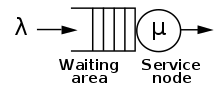
\includegraphics[width=0.4\textwidth]{Chap2_AlgorithmsPFQN/MM1_diagram.png}
\caption{Schematic of an M/M/1 queue}
\label{fig:MM1_schematic}
\end{center}
\end{figure}

The state of such a system can be uniquely defined by its population (or queue length). Assuming the service time distribution, and the arrival times are memoryless, the system can be modelled by a birth-death Markov process. The CTMC representing this is shown in figure \ref{fig:MM1_BDP}. For an open M/M/1 system with the arrival and service rates given above, several important results could be obtained. Firstly, the steady-state probabilities can be obtained by solving the global balance equations (\ref{eq:global_balance_equations}), which is uniquely described by the following set of equations:
\[ \lambda p_0 = \mu p_1\]
\[ (\lambda + \mu) p_0 = \lambda p_{n-1} + \mu p_{n+1}\]

The steady-state solution to the GBE's, which only exists if the system is stable (when \(\lambda < \mu\)) is:
\[p_n = (1-\rho) \rho^n\]
Where \(\rho = \lambda/\mu\), is the utilization. \(\rho\) represents the average proportion of time the service centre has a zero queue length.

\begin{theorem}
    Little's Law states that the average number of customers \(N\) in a stationary system is equal to the arrival rate of customers \(\lambda\) into the system multiplied by the average response time of the customer \(R\):
    \begin{equation}
        N = \lambda R
    \end{equation}
\end{theorem}

The mean queue length (\(N\)) and the mean response time (\(R\)), (using Little's Law) can be given:
\[N = \frac{\rho}{1-\rho} \quad R = \frac{1}{\mu - \lambda}\]

\begin{figure}[H]
\begin{center}
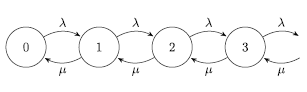
\includegraphics[width=0.5\textwidth]{Chap2_AlgorithmsPFQN/MM1_BDP.png}
\caption{Birth-death Markov process for M/M/1 queue}
\label{fig:MM1_BDP}
\end{center}
\end{figure}

\subsection{M/M/m queuing system} \label{sec:MMmQsystem}
This is a generalization of the M/M/1 system to stations with multiple servers - denoted by m. This system have service rates equal to \(\min(n,m)\mu\), where \(n\) is the instantaneous system population, and \(\mu\) is the equivalent M/M/1 service rate. The arrival process is also exponential with rate \(\lambda\). The steady state solution to the global balance equation exists if the system is stable (\(\lambda < m\mu\)), and it is given in terms of \(p_0\):
\begin{equation*}
    p_n=
    \begin{cases}
        p_0 \rho^n/n!, & n < c\\
        p_0 \rho^n/(m!m^{(n-m)}), & n \geq c
    \end{cases}
\end{equation*}
Where \(\rho = \lambda/\mu\), and the empty queue probability is given:
\[p_0 = (\sum_{n=0}^{m-1} \frac{\rho ^ n}{n!} + \frac{\rho ^ m}{(m-1)(m-\rho)})^{-1}\]

The average population of the system can be given as \(N\):
\[N = m \rho + p_m \rho / (1 - \rho)^2\]
And the mean response time \(R\):
\[R = \mu^{-1} + p_m / m \mu (1 - \rho)^2\]


\section{Queueing Networks}\label{sec:QNetworks}

Complex systems in many applications can be described in terms of a queuing network. This is a network of service centres (and variants thereof) as described above. A queuing network can be fully defined given the following inputs:
\begin{itemize}
    \item \textbf{Service centres} : The service centres have to be supplied. These service centres can be described using Kendall's notation according to the characteristics described in section \ref{sec:QueueingSystems}
    \item \textbf{Customers} : In open networks, this will be specified as an arrival distribution, whereas in closed networks, these will be described as the number of customers (these can be specified per-class in the multi-class case).
    \item \textbf{Network Topology} This describes how individual service centres connect with each other, and how customers can be routed. This is usually defined via a routing matrix. 
\end{itemize}

\subsection{Open and Closed Queuing Networks}

Open and Closed queuing networks differ in terms of how customers are available to the system. Open networks derive its customers from an external source, where arrivals are usually modelled as a Poisson arrival process. Given \(M\) service centres, this requires the specification of an external arrival rate vector \(\boldsymbol{\gamma} = (\gamma_1, \gamma_2, ... \gamma_M)\), one element per service centre. Furthermore, the routing probability matrix \(\mathbf{Q}\) \textbf{between the service centres only}, gives the traffic equations:
\[\boldsymbol{\lambda} = \boldsymbol{\gamma} + \boldsymbol{\lambda}\mathbf{Q}\]
Solving for \(\boldsymbol{\lambda}\) gives the arrival rates at individual stations in the network. \\
Closed networks, on the other hand, does not take in external arrivals, but instead circulate jobs internally. In this case, \(\boldsymbol{\gamma}\) can be set to \(\mathbf{0}\), and the traffic equations become:
\[\boldsymbol{\lambda} = \boldsymbol{\lambda}\mathbf{Q}\]
The forced-flow law also allows us to write, where \(\mathbf{v}\) is the number of visits:
\[\mathbf{v} = \mathbf{v}\mathbf{Q}\]
Since solving this entails solving a homogeneous linear system, no unique solution exists, but \(\mathbf{v}\) can usually be expressed in terms of ratios of each other, giving a set of visit ratios.

\subsection{Single-Class and Multi-Class Queuing Networks}
The analysis of queuing networks can differ depending on if a single class or multiple classes are considered. For example, in the description of service centres, the scheduling disciplines makes no difference for single class networks. However, for multi-class networks this become important. The restrictions for multi-class service centres in the context of product-form queueing networks are discussed in section \ref{sec:pfqn}. Besides, that, the concept of chains allow for jobs of different classes to switch classes within chains. However, \cite{Zahorjan1979AnNetworks} has shown that each chain can be equivalently analyzed as a single class, and multi-chain networks can be converted into an equivalent multi-class problem. Chapter 7 in \cite{Bolch2006QueueingApplications} also provides an algorithm to convert from the former to the latter network. In this project, we only consider the case where class switching is not allowed.

\subsection{Direct Solution of the Global Balance Equations}
A naive but straightforward approach to computing performance measures of queueing networks, is by modelling the network as a discrete space, continuous time homogeneous markov process. This can be done by enumerating and solving its underlying CTMC (assuming all queues are Markovian).
\\\\
Given a set of \(K\) queues, and \(R\) classes of jobs, the state space can be defined as the joint population vectors of the queues in the networks:
\begin{equation}
    \mathbf{S}_i = (\mathbf{n}_1, \mathbf{n}_2 ... \mathbf{n}_K)
\end{equation}
Where \(\mathbf{n}_k \in \mathbb{R}^R\) is the population vector of the jobs residing in service centre k.
\\\\
Let \(\mathbf{S}_{i,(nc)}\) be the population of the n-th node for class c, at state i. The transition matrix can now be defined:
\begin{equation*}
    T_{ij}=
    \begin{cases}
        \text{TR}(\mathbf{S}_i, l, c)q_{r,lk}, & \text{iff } \mathbf{S}_j \text{ is reachable from } \mathbf{S}_i \text{ through nodes l and k respectively, }\\  & \text{via the completion of a job in class c}\\
        0, & \text{otherwise}
    \end{cases}
\end{equation*}

Here \(\text{TR}(\mathbf{S}_i, l, c)\) is the (exponential) transition rate out of state \(\mathbf{S}_i\), given a class \(c\) job completes service at station l. For multi-class networks, the transition rates are, in general, station and load dependent, therefore \(\text{TR}\) is in general a function of the origin state, departing station, and departing job class. \(q_{c,lk}\) is the routing probability between nodes \(l\) and \(k\), for class c. This is covered in more detail in section \ref{sec:pfqn}.
\\\\
For a closed network with a finite number of jobs, as soon as the (finite) state space is enumerated, and the transition matrix constructed, the steady state probabilities can be computed by solving:
\begin{equation*}
    \mathbf{p}\mathbf{T'} = \mathbf{b}
\end{equation*}
Where \(\mathbf{T'}\), is the augmented transition matrix \(\mathbf{T}\) (where the last column is all 1), and \(\mathbf{b}\) is a zero vector but with the last element equals to 1, to give the normalizing condition.
\\\\
For an open network, the global balance equations will take the form of a recurrence relation similar to that of the one for the \(M/M/1\) or \(M/M/m\) queues (see sections \ref{sec:MM1Qsystem}, \ref{sec:MMmQsystem}). The solution is a closed-form expression for \(p(\mathbf{S}_i)\), the steady state probability given state \(\mathbf{S}_i\). We will focus on solution methods for closed-networks in this project.
\\\\
Given a list of states, \(\mathbf{S}_i\), the steady state probabilities \(\mathbf{p}(\mathbf{S}_i)\), performance metrics can be calculated by taking expectations and variances of various metrics such as queue lengths (\(Q_{kr}\)).
\\\\
Needless to say the solution of the (closed) network via this method is extremely costly, and grows exponentially with the number of jobs, as well as the number of service stations in the network. In the multiclass case, the size of the state space would be:
\[|\mathbf{S}| = O\bigg( \prod_c^C \binom{K_c + M -1}{K_c} \bigg)\]

Clearly this is not an option when modelling modern systems with a hundreds or thousands of service centres and classes. The idea of product form queueing networks, however, provides a convenient closed-form expression for the steady-state probability densities of a restricted, but useful class of networks, which will allow for much more efficient algorithms for performance measures.

\section{Algorithms for Product Form Queueing Networks}\label{sec:AlgorithmsPFQN}
\subsection{Product Form Queueing Networks}\label{sec:pfqn}
In this section, we introduce the notion of the product form solution for queueing networks, which will form the basis of the rest of the report. The product form solution of queueing networks expresses the steady-state probabilities of the underlying CTMC, for a single station, based on a product of the state and the parameters of individual stations. Given certain assumptions, the closed-form stationary state distribution of the CTMC is given by the product-form solution, for the single-class case as:
\begin{equation}\label{eq:pfqn_single_class}
    p(\mathbf{n}) = \frac{1}{G_{\mathbf{\theta}}} V(N) \prod_{i=1}^M g_i(n_i)
\end{equation}
Where \(\mathbf{n} = (n_1, n_2, ... n_M)\), the state of the network denoted by the number of jobs currently residing in each of the \(M\) queues. \(N = \sum_{i=1}^M n_i\). \(V(N)\) is a function of the state of the network and depend on the network's parameters and the types of service-centre/queues. \(g_i(n_i)\) is the marginal stationary queue length distribution for queue \(i\) when considered in isolation as a single queue open system. \(G = \sum_{\mathbf{n} \in \mathcal{S}_M} V(N) \prod_{i=1}^M g_i(n_i)\) is the normalizing constant of the distribution. \(\mathcal{S}_M\) is the set of all reachable states of the system. For a closed system with total population \(N\) this will be:
\[ \mathcal{S}_M = \{ \mathbf{n} \in \mathbb{N}^{MR} | n_k \geq 0, \sum_{i=1}^M n_i = N\}\]

In the special case of an open network, it can be proven that \(G=1\), and for closed networks \(V(N) = 1\). 
\\\\
For the case of a network with multiple classes of customers equation (\ref{eq:pfqn_single_class}) can be generalized to the following form:
\begin{equation}\label{eq:pfqn_multi_class}
    p(\mathbf{n}) = \frac{1}{G_{\mathbf{\theta}}} \prod_{r=1}^R V_r(N_r) \prod_{i=1}^M g_i(\mathbf{n}_i)
\end{equation}
Where \(\mathbf{n} \in \mathbb{N}^{MR}\), is the population matrix, and \(n_{kr}\) is the population of jobs of class \(r\) at station \(k\). \(V_r\) is again defined in terms of network parameters, and \(g_i\) is defined in terms of parameters of service centre \(i\) only. 

\begin{definition}
    Local balance property. A node/queue has local balance property is the departure rate from a state of of the queueing network \(\mathbf{S}_i\) due to the departure of a job of any class from node \(k\) equal to the arrival rate to this state due to an arrival of another job to the same node.
\end{definition}

The local balance property implies that the global balance equations for a state can be partitioned into a set of separate balance equations. A solution to the local balance equations is therefore also a solution to the global balance equations (the converse is not always true). \cite{Chandy1977ProductNetworks} proved that if a network only has nodes satisfying the local balance property, the network has a product form solution for the stationary state distribution.
\\\\
Two important results derived a product form solution for the case of a single-class open network (Jackson's theorem \cite{Jackson2004Jobshop-LikeSystems}), and a single-class closed network (the Gordon-Newell theorem \cite{Gordon1967ClosedServers}). 
\\\\
To introduce Jackson's theorem, we first consider a Jackson network. These are open networks of queueing systems which satisfy the following conditions:
\begin{itemize}
    \item The network has infinite capacity
    \item Every node in the network is \(M/M/m_i-FCFS\), where node \(i\) has \(m_i\) identical servers
    \item Every node in the network can have Poisson arrivals from outside, and a customer can leave the system from any node.
\end{itemize}
\begin{theorem}
    Jackson's theorem states that, a stable Jackson network consisting only of \(M/M/1-FCFS\) queues, (i.e. \(\lambda_i < \mu_i \; \forall i = 1, .. M\)), the product form solution of the network is given:
    \begin{equation}
        P(\mathbf{n}) = \prod_{i=1}^M (1-\rho_i) \rho_i^{n_i}
    \end{equation}
\end{theorem}

The Gordon-Newell theorem extends this result to a closed-system of \(M/M/m-FCFS\) queues with a fixed number of customers \(N\).
\begin{theorem}
    The Gordon-Newell theorem for closed-networks of single-class \(M/M/m-FCFS\) queues states that the stationary state probability this network is given by the product form solution:
    
    \begin{equation}\label{eq:GNPFQN}
        P(\mathbf{n}) = \frac{1}{G_{\boldsymbol{\theta}}(N)} \prod_{i=1}^M \bigg( \frac{\theta_i^{n_i}}{\prod_{j=1}^{n_i} \beta_i(j)} \bigg)
    \end{equation}
    
    Where \(\theta_i\) is the service demand placed on node \(i\) by a single job, given by the utilization law, where \(\lambda(N)\) is the overall throughput of the system:
    \begin{equation*}
        \theta_i = \rho_i \lambda(N)
    \end{equation*}
    
    And \(\beta_i(j) = \min(m_i, j)\) is a scaling factor for nodes with \(m_i\) servers.
    
    The normalizing constant \(G_{\boldsymbol{\theta}}(N)\) is given by summing the product terms in equation (\ref{eq:GNPFQN}).
    
\end{theorem}

\begin{proof}
    The proof of the above theorems involve showing that the formulas for \(P(\mathbf{n})\) above satisfy the global balance equations for the underlying CTMC. This is given in full in \cite{Bolch2006QueueingApplications} Chapter 7.
\end{proof}

The BCMP theorem, named after the authors that first theorized it \cite{Baskett1975OpenCustomers}, , expanded the product form solution even further to include multi-class networks and networks of types other than \(M/M/m-FCFS\) servers. These are grouped into 4 types of networks, collectively referred to as BCMP networks.

\begin{definition}
    BCMP networks are open, closed or mixed multiclass networks that consist of queues which fall into one of the following types:
    \begin{itemize}
        \item \textbf{Type 1:} FCFS queuing discipline \(-/M/m-FCFS\). For multiclass networks, all job classes must have the same service rate \(\mu_i\).
        \item \textbf{Type 2:} Processor-sharing (PS) queuing discipline and arbitrary phase-type distribution \(-/G/1-PS\)
        \item \textbf{Type 3:} Infinite server (IS) and arbitrary phase-type distribution -/G/\(\infty\)
        \item \textbf{Type 4:} Last come first serve with pre-emptive resume (LCFS-PR) and arbutrary phase-type distribution \(-/G/1-LCFS\).
    \end{itemize}
\end{definition}

\begin{theorem}
    The BCMP theorem states that, for BCMP networks, the steady state product form solution is given by :
    \begin{equation} \label{eq:BCMP_PFQN}
        p(\mathbf{n}) = \frac{1}{G_{\boldsymbol{\theta}}(\mathbf{N})} \prod _ {i=1} ^ M F_i(\mathbf{n_i})
    \end{equation}
    Where \(\mathbf{n} = (\mathbf{n}_1, ... \mathbf{n}_M)\) And the function \(F_i(\mathbf{n}_i)\) is given by:
    \begin{equation}
        F_i(\mathbf{n}_i)=
        \begin{cases}
            \frac{1}{\beta_i(n_i)} n_i! \prod _{r=1} ^ R  \frac{\theta_{ir}^{k_{ir}}}{n_{ir}!} & \text{Type 1}\\\\
            k_i! \prod _{r=1} ^ R  \frac{\theta_{ir}}{(k_{ir}!)} & \text{Type 2,4}\\\\
            \prod _{r=1} ^ R \frac{\theta_{ir}}{(k_{ir}!)} & \text{Type 3}\\
        \end{cases}
    \end{equation}
    Where the job service demands \(\theta_{ir}\) can be expressed in terms of visit ratios and service rates:
    \begin{equation*}
        \theta_{ir} = \frac{v_{ir}}{\mu_{ir}}
    \end{equation*}
\end{theorem}

The proof of this theorem is complex and outside of the scope of this project. The original proof \cite{Baskett1975OpenCustomers} was given by the authors of the theorem and involved checking that the local and global balance equations of the underlying CTMC are satisfied by the above product form solution.

\subsection{The Normalizing Constant and Performance Indices}
The normalizing constant \(G\) of the product-form solution for queueing networks is of paramount importance in applications involving network modelling. Not only does this quantity allow us to compute the actual steady-state probabilities of the network, it arises in the computation of network performance indices such as the average queue length \(Q_{kr}\), and overall class throughputs \(\lambda_r\). For closed queueing networks, this is given \cite{Reiser1975QueuingAlgorithms}:

\begin{equation}
    \lambda_r(\mathbf{N}) = \frac{G_{\boldsymbol{\theta}}(\mathbf{N} - \mathbf{1}_r)}{G_{\boldsymbol{\theta}}(\mathbf{N})}
\end{equation}
\begin{equation}
    Q_{kr}(\mathbf{N}) = \theta_{kr} \frac{G^{(+k)}_{\boldsymbol{\theta}}(\mathbf{N} - \mathbf{1}_r)}{G_{\boldsymbol{\theta}}(\mathbf{N})}
\end{equation}

Where \(\mathbf{1}_r \in \mathbb{N}^r\) is a vector that has all zeros except for a \(1\) in position \(r\). \(G^{(+k)}_{\boldsymbol{\theta}}(\mathbf{N})\) Is the normalizing constant for a network augmented with an extra node \(k\). Average response times and utilizations can be computed in terms of \(Q_{kr}(\mathbf{N})\) and \(\lambda_r(\mathbf{N})\) via the application of the fundemental laws, e.g. Little's Law and the Utilization Law.
\\\\
While it is true that there are algorithms \cite{Reiser1975QueuingAlgorithms, Chow1983ApproximationsNetworks, Chandy1982Linearizer:Systems, Sevcik2002SolutionAlgorithm} that can compute these average performance indices, \(Q_{kr}\) and \(\lambda_r\), more efficiently than \(G\) can be computed, there are still many explicit uses of \(G\) of interest. 
\\\\
Casale \cite{Casale2017AcceleratingMethods} provides one such motivating example. Suppose we are provided with a set of \(L\) state samples \(\mathbf{n}^{(l)} \in \mathcal{S}_M, \; l=1,...L\), assuming zero delays, and a network of single-server nodes, the log-likelihood of the samples given a demand matrix \(\boldsymbol{\theta}\) ( (\(\log P(\{\mathbf{n}^{(l)} \forall l=1,...L \} | \boldsymbol{\theta})\) or \(\mathcal{L}(\boldsymbol{\theta})\) ) can be written:
\[\mathcal{L}(\boldsymbol{\theta}) = \sum_{l=1}^L \log C(\mathbf{n}^{(l)}) + L \sum_{k} \sum_{r} \widetilde{Q}_{kr} \log \theta_{kr} - L \log G_{\boldsymbol{\theta}}(\mathbf{N})\]

Where \(\widetilde{Q}_{kr} = \sum_{l} n_{kr}^{(l)}/L\) is the \textit{measured} mean queue-length of class \(r\) at node \(k\).

\subsection{Exact Algorithms}\label{sec:exact_algos}
\textit{{\large Convolution Algorithm}}\\\\
The Convolution Algorithm (CA) makes use of the product form solution of the networks described in \ref{sec:pfqn} to compute the normalizing constant \(G_{\boldsymbol{\theta}}(\mathbf{N})\). Given a product-form solution of a closed product-form queueing network:
\begin{equation}
    p(\mathbf{n}) = \frac{1}{G_{\boldsymbol{\theta}}(\mathbf{N})} \prod_{k=1}^M g_i(\mathbf{n}_i)
\end{equation}

Where the normalizing constant \(G_{\boldsymbol{\theta}}(\mathbf{N})\) can be given in the explicit summation, (Where \(N_r\) is the total population of jobs of class \(r\)):
\[G_{\boldsymbol{\theta}}(\mathbf{N}) = \sum_{\substack{\mathbf{n} \geq \mathbf{0}\\ \sum_r{n_{kr}} = N_r}} \prod_{i=1}^M g_i(\mathbf{n_i})\]

This can be re-arranged to give the following recursive summation:
\[ G_{\boldsymbol{\theta}}(M, \mathbf{N}) =  \sum_{\mathbf{0} \leq \mathbf{j} \leq \mathbf{N}} g_i(\mathbf{j}) G_{\boldsymbol{\theta}}(M-1, \mathbf{N-j})\]

Where \(G_{\boldsymbol{\theta}}(M-1, \mathbf{N})\) is the normalizing constant for a network with the \(M^{th}\) queue removed. And the initial conditions are as follows:
\[G_{\theta}(1,\mathbf{N}) = g_1(\mathbf{n}_1) \quad G_{\theta}(\cdot,\mathbf{0}) = 1\]
For a model consisting only of load independent stations, the equation simplifies to:
\[G_{\boldsymbol{\theta}}(M, \mathbf{N}) = G_{\boldsymbol{\theta}}(M-1, \mathbf{N}) + \sum_{r=1}^R \theta_{kr} G_{\boldsymbol{\theta}}(M, \mathbf{N-1_r}) \]

This method, while far more efficient than the explicit summation of the terms for each state, still grows like \(O(\prod_{r=1}^R N_r^2)\) for the general case, and \(O(MR \prod_{r=1}^R N_r)\) in the case with load-independent demands. Space requirements = \(O(\prod_{r=1}^R N_r)\), like the number of subproblems.
\\\\
\textit{{\large Mean Value Analysis Algorithm}}\\\\
The mean value analysis (MVA) algorithm first presented in \cite{Reiser1980Mean-ValueNetworks} bypasses the need to compute the normalizing constant, and instead computes the average performance indices directly, through a multi-dimensional recursion. The MVA algorithm is given here for BCMP networks.
\\\\
This is defined as follows \cite{Lazowska1984QuantitativeModels}:
The node residence time \(W_{kr}(\mathbf{N})\) is given:
\begin{equation}\label{eq:MVA_step1}
    W_{kr}(\mathbf{N}) = 
    \begin{cases}
        \theta_{kr} & \text{if node k is a Type 3 node}\\
        \theta_{kr}(1 + A_{kr}(\mathbf{N})) & \text{if node k is a Type 1,2 or 4 node, } m_k = 1\\
        \frac{\theta_{kr}}{m_i}(1 + A_{kr}(\mathbf{N})) & \text{if node k is a Type 1 node, } m_k > 1
    \end{cases}
\end{equation}
Where \(A_{kr}(\mathbf{N})\) is the arrival instant queue length for class \(r\) at node \(k\). Turns out there are several techniques to obtain an exact and approximate solution to this set of equations, and that lies in the way \(A_{kr}(\mathbf{N})\) is computed.
\\\\
The other equations involved in this recursion is based on Little's Law:
\begin{equation}\label{eq:MVA_step2}
  \lambda_{r}(\mathbf{N}) = \frac{N_r}{\sum_{k=1}^M} W_{kr}(\mathbf{N})  
\end{equation}
\begin{equation}\label{eq:MVA_step3}
K_{kr}(\mathbf{N}) = \lambda_{r}(\mathbf{N}) W_{kr}(\mathbf{N})
\end{equation}

In exact MVA, \(A_{kr}(\mathbf{N})\) is calculated exactly according to the following equation:
\[A_{kr}(\mathbf{N}) = 
\begin{cases} 
Q_{kr}(\mathbf{N-1_r}) & \text{Type 1,2,4 nodes, with }m_k = 1 \\ 
Q_{kr}(\mathbf{N-1_r}) + \sum_{j=0}^{m_i-2} (m_k - j - 1)p_k(j|\mathbf{N-1_r}) & \text{Type 1 nodes, with } m_k = 1
\end{cases}
\]
Here the marginal probability that there are \(j\) jobs at the \(k^{th}\) node, \(0 \leq j \leq m_i-1\) given that the network is in state \(\mathbf{N>0}\)
\[
p_k(j|\mathbf{N}) = 
\begin{cases} 
\frac{1}{j} \bigg[ \sum_{k=1}^R \theta_{kr} \lambda_r(\mathbf{N}) p_k(j-1|\mathbf{N-1_r}) \bigg] & j > 0\\ 
1 - \frac{1}{m_k} \bigg[ \sum_{r=1}^R \theta_{kr} \lambda_r(\mathbf{N}) + \sum_{j=1}^{m_k-1}(m_k - j)p_k(j|\mathbf{N})\bigg]  & j=0 
\end{cases}
\]
And base case:
\[ p_k(j|\mathbf{0}) =  \begin{cases} 1  & j=0 \\ 0 & \text{otherwise} \end{cases} \]
The time complexity of this algorithm is \(O(RM \prod_{r=1}^R N_r)\), and the space complexity is \(O(M \prod_{r=1}^R N_r)\). Both time and space complexity for MVA is also exponential in the number of classes, but grows less quickly for the load-dependent (multiserver/IS) case than the convolution algorithm.
\\\\
The approximate solution of \(A_{kr}(\mathbf{N})\) will be discussed in section \ref{sec:approx_algos}. 
\\\\
\textit{{\large RECAL Algorithm}}
\\\\
In this algorithm, first presented in \cite{Conway1986RECAL---aNetworks}, each queue is completely associated with a single, self-looping class. The RECAL algorithm uses the following recursion algorithm:
\begin{equation}
    N_r G_{\boldsymbol{\theta}}(\mathbf{m,N}) = \sigma_r G_{\boldsymbol{\theta}}(\mathbf{m,N-1_r}) + \sum_{k=1}^M (1 + m_k) \theta_{kr} G_{\boldsymbol{\theta}}(\mathbf{m+1_k,N-1_r})
\end{equation}
Where \(G_{\boldsymbol{\theta}}(\mathbf{m,N})\) is the normalizing constant of a queueing network of load-independent servers, and \(\mathbf{m} \in \mathbb{N}^M\) is the multiplicity vector indicating the count of the number of each server. \(\sigma_r\) indicates the mean delay experienced by each class in the network. The initial conditions are given:
\[G(\mathbf{0}, \mathbf{N}) = \prod_{r=1}^R \frac{\theta_r^{N_r}}{N_r!} \quad G(\cdot, \mathbf{0}) = 1 \]
\\\\
This algorithm has time and space complexity \(O(N^M)\), making it suitable only for networks with a small number of queues.
\\\\
\textit{{\large Method of Moments Algorithm}}\\\\
A number of variants of this method exists, given in \cite{Casale2011ANetworks, Casale2011ANetworksb, Casale2009CoMoM:Models}. This method applies the convolution algorithm and RECAL algorithm to a set of normalizing constants that differ for the lements and compotision of \(\boldsymbol{\theta}\) and \(\mathbf{N}\). Different rules exist to define this set of normalizing constants, called the \textit{basis}. Given that the normalizing constants in the basis are given in the vector \(\mathbf{g(N)}\), the method of moments defines a matrix recurrence relation.
\[\mathbf{A(\boldsymbol{\theta}, N)g(N)} = \mathbf{B(\boldsymbol{\theta}, N)g(N-1_r)}\]
For any \(1 \leq r \leq R\), and \(\mathbf{g(0)}\) are given by the initial conditions as defined in the convolution and RECAL algorithms. The square matrices \(\mathbf{A(\boldsymbol{\theta}, N)g(N)}\) and \(\mathbf{B(\boldsymbol{\theta}, N)g(N)}\) are square matrices, and decrease in size as the recurrence progresses. 
\\\\
Provided that \(\mathbf{A(\boldsymbol{\theta}, N)}\) is invertible at all steps of the recursion, it is possible to compute \(\mathbf{g(N)}\) and obtain \(\mathbf{G_{\boldsymbol{\theta}}(N)}\) from the elements of \(\mathbf{g(N)}\). A required condition for invertibility if that \(\theta_{ir} \neq \theta_{jr}, \forall i,j,r, i \neq j\). This algorithm has a theoretical time complexity of \(O(N)\) time and \(O(1)\) space. However, since the method of moments algorithm requires the above recurrence relation to be carried out using exact arithmetic, a significant portion of the cost could go to performing calculations using exact representations.

\subsection{Approximate and Randomized Algorithms} \label{sec:approx_algos}

\textit{{\large Approximate Mean Value Analysis Algorithm}}\\\\
Approximate Mean Value Analysis (AMVA) algorithms work by providing a reasonable estimate to the arrival instant queue lengths \(A_{kr}(N)\). In exact MVA, this was computed using exact recursion. The Chow algorithm \cite{Chow1983ApproximationsNetworks} approximates this as:
\[A_{kr}(\mathbf{N}) = Q_{kr}(\mathbf{N-1_r}) \approx Q_{kr}(\mathbf{N}) \]
Based on the assumption that the average queue lengths for a network with one less customer is almost identical to that of a network with one less customer. This assumption is reasonable for a model with a large number of customers.
\\\\
The above approximation can be then used in the system of equations (\ref{eq:MVA_step1}, \ref{eq:MVA_step2}, \ref{eq:MVA_step3}), which can be solved iteratively until the required tolerance between values of successive iterations falls below a certain threshold.
\\\\
The Brad-Schweitzer Algorithm \cite{Schweitzer1993AQueues} provides a slightly better approximation to \(A_{kr}(\mathbf{N})\):
\[Q_{kr}(\mathbf{N-1_r}) = \frac{N_r-1}{N_r} Q_{kr}(\mathbf{N}) + \sum_{\substack{j=1\\ j\neq r}}^R Q_{kr}(\mathbf{N})\]
Which provides more accurate esimates than the Chow AMVA algorithm at the cost of additional computation complexity per iteration. Better approximations to the MVA system of equations are provided in \cite{Chandy1982Linearizer:Systems} which include performing calculations of \(O(MR^2)\) to obtain even better approximations at the cost of more complexity.
\\\\
\textit{{\large Monte Carlo Methods}}\\\\ 
Monte Carlo integration methods for the normalizing constant were first introduced in \cite{Ross1994MonteNetworks}. These randomized methods use the following integral form derived in \cite{McKenna1984AsymptoticNetworks}. 
\begin{equation}\label{eq:MCI_form_Ross}
    G_{\boldsymbol{\theta}}(\mathbf{N}) = \frac{1}{\prod_{i=1}^R N_r!} \int_{\mathbb{R}_+^K} e^{-y} \prod_{r=1}^R \bigg( \sigma_r + \sum_{k=1}^K \theta_{kr} y_k \bigg)^{N_r} d \mathbf{y}
\end{equation}

Where \(\mathbb{R}_+^K = \{ \mathbf{y} \in \mathbb{R}^K | \mathbf{y \geq 0}\} \) is the non-negative orthant of the K-dimensional real space, \(\mathbb{R}^K\), and \(y = \sum_k y_k\). \(\sigma_r = \sum_{k=K+1}^M \theta_{kr}\) is the sum of the class-\(r\) demands at all infinite servers. The above expression is obtained by considering the form of the normalizing constant for networks of single and infinite server queues only:
\begin{equation*}
    G_{\boldsymbol{\theta}}(\mathbf{N}) = \sum_{\mathbf{n} \in \mathcal{S}_M} \prod_{i=1}^K n_i! \prod_{k=1}^M \prod_{r=1}^R \frac{\theta_{n_{kr}}}{n_{kr}!}
\end{equation*}

Expression (\ref{eq:MCI_form_Ross}) is obtained by expression the \(n_i!\) terms in the above form of the normalizing constant, in the integral form of the gamma function, and subsequently by repeated application of the multinomial theorem:
\begin{equation*}
    \bigg( \sum_{k=1}^K x_k \bigg)^V = V! \sum_{\mathbf{v \geq 0}, v=V} \prod_{k=1}^K \frac{x_k}{v_k!}
\end{equation*}

The integral form of the normalizing constant (\ref{eq:MCI_form_Ross}) can be efficiently evaluated using importance sampling with the following sampling distribution:
\[p(\mathbf{y}) = \prod_{i=k}^K p_k(y_k)\]
And \(p_k(y_k)\) is the PDF of a scalar exponential distribution:
\[p_k(y) = \gamma_k e^{-\gamma_k y}\]
Where \(\gamma_k\) are parameters that can be tuned to minimize variance in the computed integral \cite{Ross1994MonteNetworks}. Typically a sample size of \(10^5-10^7\) is required in order to approximate \(G_{\boldsymbol{\theta}}(\mathbf{N})\) with reasonable variance. 
\\\\
In a similar vein to \cite{Ross1994MonteNetworks}, this project focuses on applying Monte Carlo integration of an integral form of the normalizing constant. However, unlike what has been done before, this project builds on novel integral forms of the normalizing constant \(G_{\boldsymbol{\theta}}(\mathbf{N})\) to achieve a better sampling efficiency than what was achieved in previous randomized methods. These will be described in detail in the following chapters.



%%%%%%%%%%%%%%%%%%%%%%%%%%%%%%%%%%%%
\chapter{Integrals On the Simplex}\label{sec:Chapter3}

In this chapter, novel integral forms of the normalizing constant for 3 types of networks are presented: single-server networks (section \ref{sec:single_server_simplex_integral}), single-server networks with delay(section \ref{sec:inf_server_simplex_integral}), and multi-server networks (section \ref{sec: multi_server_simplex_integral}), with the main results being presented in equations (\ref{eq:start_simplex_single_server}), (\ref{eq:start_simplex_inf_server}), and (\ref{eq:multi_server_NC}), respectively. These take the form of integrals of functions over the \(K\)-dimensional unit simplex (denoted by \(\Delta_K\) or \(\mathbb{S}^K\)), for a network with \(K\) nodes/queues.
\\\\
These integral forms of the normalizing constant \(\mathbf{G}_{\boldsymbol{\theta}}(\mathbf{N})\) forms the basis of this project's approach, and will be used and referenced extensively throughout this report.
\\\\
The original proofs of the single-server and single and infinite (delay) server networks were given in \cite{Casale2017AcceleratingMethods}. Here, an alternative proof is presented, which uses the Dirichlet Integral identity over the simplex in equation (\ref{eq:dirichlet_simplex_integral}). 

\section{Preliminaries}

The purpose of this section is to summarize several important identities that are required to derive the simplex integral form of the normalizing constant.
\\\\
The multinomial theorem states that, for any set of real numbers \((x_1, x_2 ... x_k)\), and nonnegative integer \(V\):
\begin{equation}\label{eq:mt}
    \bigg( \sum_{k=1}^K x_k \bigg)^V = V! \sum_{\substack{\mathbf{v} \geq 0, \\ \sum_k^K v_k = V}}\prod_{k=1}^K \frac{x_k^{v_k}}{v_k!}
\end{equation}

\begin{theorem} \label{theorem:multinomial_2}
The multinomial theorem implies the following. For any set of real numbers \((a_1, a_2 ... a_k)\), and nonnegative integer \(N\)
    \begin{equation} \label{eq:multinomial_2}
        a_1^{N_1} a_2^{N_2} ... a_R^{N_R} = \frac{1}{N!} \frac{\partial^{N_1}....\partial^{N_R}}{\partial t_1^{N_1}....\partial t_R^{N_R}}\bigg( \sum_{i=1}^R a_i t_i \bigg)^N
    \end{equation}
\end{theorem}

\begin{proof}
    Taking the term on the right hand side of (\ref{eq:multinomial_2}), using (\ref{eq:mt}), we can write:
    \begin{equation}\label{eq:differentiation_filter}
        \frac{1}{N!} \frac{\partial^{N_1}....\partial^{N_R}}{\partial t_1^{N_1}....\partial t_R^{N_R}}\bigg( \sum_{i=1}^R a_i t_i \bigg)^N = \frac{1}{N!} \frac{\partial^{N_1}....\partial^{N_R}}{\partial t_1^{N_1}....\partial t_R^{N_R}} \bigg( N! \sum_{\substack{\mathbf{n} \geq 0, \\ \sum_i^R n_r = N}}\prod_{i
        =1}^R \frac{(a_i t_i)^{n_i}}{n_i!} \bigg)
    \end{equation}
    And the fact that 
    \begin{equation*}
        \frac{\partial^{N_i}}{\partial t_i ^{N_i}} \prod_{i=1}^R t^{n_i} = 
        \begin{cases}
             \prod_i^R N_i! & \text{if } n_i = N_i, \forall i=1...R \\
            0 & \text{otherwise}
        \end{cases}
    \end{equation*}
    
    We recover the left hand side of (\ref{eq:multinomial_2}).
    
\end{proof}

Another important result is the identity of the definite integral over the simplex \(\Delta_K\):
\begin{equation} \label{eq:dirichlet_simplex_integral}
    \int_{\Delta_K} \prod_{k=1}^K u_k^{n_k} d\mathbf{u} = \frac{\prod_{k=1}^K n_k!}{\big( \sum_{k=1}^K n_k +K -1 \big)!}
\end{equation}
 The \(K\)-dimensional unit simplex is defined as a set of \(K\)-dimensional points \(\mathbf{u}\) in the positive quadrant, such that all such points have sum of their components equal to 1:
 \begin{equation*}
    \Delta_K = \bigg  \{ \mathbf{u} : \forall u_i > 0, \sum_{i=1}^K u_i = 1 \bigg \}
\end{equation*}
\subsection{Finite Differences}

Another important concept required for the derivation of results in section \ref{sec: multi_server_simplex_integral} is that of finite differences. It may be seen as the discrete analog of continuous derivatives in calculus. 

\begin{definition}
    For a discrete function \(f_k\), defined at discrete points \(k \geq 1\) The \(n\)-th forward difference of a function is given by the recurrence relation:
    \[\Delta_k^n = \Delta_k^{n-1} f_{k+1} - \Delta_k^{n-1} f_{k}\]
    Where the first-order difference is given:
    \[\Delta_k f_k = f_{k+1} - f_k\]
\end{definition}

An alternative formulation of the forward difference is that of the alternating sum:
\begin{equation}
    \Delta_k^n f_k = \sum_{k=0}^n (-1)^{n-k} \begin{pmatrix} n \\ k\end{pmatrix} f_k
\end{equation}

A result of Euler's formula for \(n\)-th differences of powers is given in \cite{Gould1978EulersPowers} for the case where \(f_k\) is a polynomial of the form \(k^m\):
\begin{equation}\label{eq:euler_power_diffrences}
    \Delta_k^n k^m = \sum_{k=0}^n (-1)^{n-k} \begin{pmatrix} n \\ k\end{pmatrix} k^m = 
    \begin{cases}
    0 & \text{if } m < n \\
    n! & \text{if } m=n
    \end{cases}
\end{equation}

To generalize to multivariate polynomials \(p(\mathbf{k})\), where \(\mathbf{k} = (k_1, ... k_m)\), we introduce the notation for the composition of \(m\) forward differences:
\begin{equation}
    \Delta_\mathbf{k}^\mathbf{n} p(\mathbf{k}) = \Delta_{k_m}^{n_m} \Delta_{k_{m-1}}^{n_{m-1}} ... \Delta_{k_1}^{n_1} p(\mathbf{k})
\end{equation}

The repeated application of Euler's formula (\ref{eq:euler_power_diffrences}) on each \(\Delta^n_k\) operator leads to the following proposition from \cite{Casale2018ExplicitRepresentations}:
\begin{theorem} \label{theorem:multivar_euler_power_differnces}
    Let \(p(\mathbf{k})\) be a polynomial of degree \(n = n_1 + ... + n_m\) in the discrete variable \(\mathbf{k} = (k_1, ... k_m)\). If we denote the coefficient of the monomial \(k_1^{n_1}k_2^{n_2}...k_M^{n_m}\) as \(a_0\) , then
    \begin{equation}
        \Delta_\mathbf{k}^\mathbf{n} p(\mathbf{k}) = \sum_{\mathbf{0 \geq k \neq n}} (-1)^{n-k} \prod_{i=1}^m \begin{pmatrix} n_i \\ k_i \end{pmatrix} p(\mathbf{k}) = a_0 \prod_{i=1}^m n_i!
    \end{equation}
\end{theorem}

A formal, inductive prove on the above theorem is given in \cite{Casale2018ExplicitRepresentations}. A consequence of the above theorem is that for set of \(m\) arbitrary coefficients \(\mathbf{u} = (u_1, ... , u_m)\):
\begin{equation}\label{eq:power_differences_multinomial}
    \frac{1}{n!} \Delta_{\mathbf{k}}^{\mathbf{n}} \bigg( \sum_{i=1}^m k_i u_i\bigg)^n =
    \frac{1}{n!} \Delta_{\mathbf{k}}^{\mathbf{n}} \sum_{\substack{\mathbf{v \leq 0} \\ v=n}} \frac{n!}{\prod_{j=1}^m v_j!} \prod_{i=1}^m k_i^{v_i} u_i^{v_i} = \prod_{i=1}^m u_i^{n_i}
\end{equation}

\section{Integral form for Single Server Node Networks} \label{sec:single_server_simplex_integral}

The integral form for single-server node networks over the \(K\)-dimensional unit simplex \(\Delta_K\) is given in the theorem below, and a proof is presented:

\begin{theorem} \label{theorem:simplex_single_server}
In a multiclass closed queueing network with K single-server nodes
    \begin{empheq}[box=\mymath]{equation}\label{eq:start_simplex_single_server}
        G_{\boldsymbol{\theta}}(\mathbf{N}) =  \frac{(N+K-1)!}{N_1! ... N_R!} \int_{\Delta_K}\prod_{r=1}^R \bigg( \sum_{k=1}^K \theta_{kr} u_k \bigg)^{N_r} d\mathbf{u}
    \end{empheq}
Where \(\Delta_K = \{ \mathbf{u} \in \mathbb{R}^K | u_i \geq 0, \sum_{i=1}^K u_i = 1\}\) is the unit simplex.
\end{theorem}

\begin{proof}
    We prove that (\ref{eq:start_simplex_single_server}) is equivalent to the original form of the normalizing constant:
    \begin{equation}\label{eq:end_proof}
    G_{\boldsymbol{\theta}}(\mathbf{N}) =  \sum_{\substack{n_{kr} \geq 0 \\ \sum_k n_{kr} = N_r \\ \forall r= 1...R}} \prod_{i=1}^{K} n_i! \prod_{k=1}^{M} \prod_{r=1}^{R} \frac{\theta_{kr}^{n_{kr}}}{n_{kr}!}
    \end{equation}
    
    Where \(\mathbf{N} = (N_1, N_2 \dot ,N_R)\). And \(N = \sum_r^R N_r\). 
    \\\\
    Starting from (\ref{eq:start_simplex_single_server}), we first write the integral on the right hand side as:
    \begin{equation*}
        I_{\boldsymbol{\theta}}(\mathbf{N}) =  \int_{\Delta_K}\prod_{r=1}^R \bigg( \sum_{k=1}^K \theta_{kr} u_k \bigg)^{N_r} d\mathbf{u}
    \end{equation*}
    
    Using the multinomial theorem of the form (\ref{eq:multinomial_2}), this can be written (after exchanging the order of integration and differentiation)
    \begin{equation}
        I_{\boldsymbol{\theta}}(\mathbf{N}) =  \frac{1}{N!} \frac{\partial^{N_1}....\partial^{N_R}}{\partial t_1^{N_1}....\partial t_R^{N_R}} \int_{\Delta_K}  \bigg( \sum_{r=1}^R \sum_{k=1}^K \theta_{kr} u_k t_r \bigg)^{N} d\mathbf{u}
    \end{equation}

    Applying the multinomial theorem (\ref{eq:mt}) on the sum in the brackets, we get:
    \begin{equation}
        I_{\boldsymbol{\theta}}(\mathbf{N}) =  \frac{1}{N!} \frac{\partial^{N_1}....\partial^{N_R}}{\partial t_1^{N_1}....\partial t_R^{N_R}} \int_{\Delta_K} N! \sum_{n_{kr} \geq 0 \\ \sum n_{kr} = N} \prod_{r=1}^R \prod_{k=1}^K \frac{\big(  \theta_{kr} u_k t_r \big)^{n_{kr}}}{n_{kr}!} d\mathbf{u}
    \end{equation}
    
    The integrand then becomes (after switching integration and summation, and factorising out \(u_k\)):
    \begin{equation}
        I_{\boldsymbol{\theta}}(\mathbf{N}) = \frac{\partial^{N_1}....\partial^{N_R}}{\partial t_1^{N_1}....\partial t_R^{N_R}}  \sum_{n_{kr} \geq 0 \\ \sum n_{kr} = N} \int_{\Delta_K} \prod_{k=1}^K u_k^{n_k} d\mathbf{u} \prod_{r=1}^R \prod_{k=1}^K \frac{\big(  \theta_{kr} t_r \big)^{n_{kr}}}{n_{kr}!} 
    \end{equation}
    
    Using (\ref{eq:dirichlet_simplex_integral}) this becomes:
    \begin{align}
        %%%%%%
        I_{\boldsymbol{\theta}}(\mathbf{N}) 
        & = \frac{\partial^{N_1}....\partial^{N_R}}{\partial t_1^{N_1}....\partial t_R^{N_R}}  \frac{1}{(N+K-1)!}  \sum_{\substack{n_{kr} \geq 0 \\ \sum n_{kr} = N}} \prod_{k=1}^K n_k! \prod_{r=1}^R \prod_{k=1}^K \frac{\big(  \theta_{kr} t_r \big)^{n_{kr}}}{n_{kr}!} \\
        %%%%%%
        & = \frac{\partial^{N_1}....\partial^{N_R}}{\partial t_1^{N_1}....\partial t_R^{N_R}}  \frac{1}{(N+K-1)!}  \sum_{\substack{n_{kr} \geq 0 \\ \sum n_{kr} = N}} \prod_{r=1}^R t_r^{n_r} \prod_{k=1}^K n_k! \prod_{r=1}^R \prod_{k=1}^K \frac{ \theta_{kr}^{n_{kr}}}{n_{kr}!} 
    \end{align}
    
    Using \ref{eq:differentiation_filter}, the terms in the summation where \(n_r \neq N_r, \forall r=1...R\) goes to zero, and we are left with
    \begin{equation}
        I_{\boldsymbol{\theta}}(\mathbf{N}) 
        = \frac{N_1!N_2!...N_R!}{(N+K-1)!}  \sum_{\substack{n_{kr} \geq 0 \\ \sum_k n_{kr} = N_r \\ \forall r= 1...R}} \prod_{k=1}^K n_k! \prod_{r=1}^R \prod_{k=1}^K \frac{ \theta_{kr}^{n_{kr}}}{n_{kr}!} 
    \end{equation}
    
    Combining this back with :
    \begin{equation}
        G_{\boldsymbol{\theta}}(\mathbf{N}) =  \frac{(N+K-1)!}{N_1! ... N_R!} I_{\boldsymbol{\theta}}(\mathbf{N}) 
    \end{equation}

    Gives us the original form of the normalizing constant (\ref{eq:end_proof}). 
\end{proof}

\section{Integral form for Networks with Infinite Server Nodes} \label{sec:inf_server_simplex_integral}

In this section, we prove the integral form for single-server node networks with infinite (delay) server present.

\begin{theorem}
In a multiclass closed queueing network with M nodes in total : K single-server nodes, and \(M-K\) infinte server nodes. The normalizing constant can be expressed by the integral:
    \begin{empheq}[box=\mymath]{equation}\label{eq:start_simplex_inf_server}
        G_{\boldsymbol{\theta}}(\mathbf{N}) =  \int_{\Delta_K} \int_{v=0}^{\infty} \frac{e^{-v} v^{K-1}}{N_1! ... N_R!} \prod_{r=1}^R \bigg( \sigma_r + v \sum_{k=1}^K \theta_{kr} u_k \bigg)^{N_r} dv d\mathbf{u} 
    \end{empheq}
    Where \(\sigma_r = \sum_{k=K+1}^M \theta_{kr}\), the sum of the infinite server node demands per class.
\end{theorem}

\begin{proof}
    We can write (\ref{eq:start_simplex_inf_server}) as:
    \begin{equation}
        G_{\boldsymbol{\theta}}(\mathbf{N}) = \frac{1}{N_1! ... N_R!} \mathbf{I(N)}
    \end{equation}
    Where:
    \begin{equation}
        \mathbf{I(N)} = \int_{\Delta_K} \int_{v=0}^{\infty} e^{-v} v^{K-1} \prod_{r=1}^R \bigg( \sum_{k=1}^M \theta_{kr} q_k \bigg)^{N_r} dv d\mathbf{u} 
    \end{equation}
    \[q_k = 
    \begin{cases}
        u_k v & k \leq K\\
        1 & k > K\\
    \end{cases}\]
    
    Using the multinomial theorem (\ref{eq:mt}) and (\ref{eq:multinomial_2}) in the same way as it was used in section \ref{sec:single_server_simplex_integral}, we can write:
    \begin{equation}
        \mathbf{I(N)} = \frac{\partial^{N_1}....\partial^{N_R}}{\partial t_1^{N_1}....\partial t_R^{N_R}} \sum_{\substack{n_{kr} \geq 0 \\ \sum n_{kr} = N}} \int_{\Delta_K} \int_{v=0}^{\infty} e^{-v} v^{K-1} \prod_{r=1}^R \prod_{k=1}^M \frac{(\theta_{kr} t_r q_k)^{n_{kr}}}{n_{kr}!}  dv d\mathbf{u} 
    \end{equation}
    
    Factorizing out \(v\) and \(u_k\) from \(q_k\):
    \begin{equation}
        \mathbf{I(N)} = \frac{\partial^{N_1}....\partial^{N_R}}{\partial t_1^{N_1}....\partial t_R^{N_R}} \sum_{\substack{n_{kr} \geq 0 \\ \sum n_{kr} = N}}  \int_{\Delta_K} \bigg( \prod_{i=1}^K u_i^{n_i} \bigg) d\mathbf{u} \int_{v=0}^{\infty} e^{-v} v^{n +K-1} dv \prod_{r=1}^R \prod_{k=1}^M \frac{(\theta_{kr} t_r)^{n_{kr}}}{n_{kr}!}  
    \end{equation}
    
    Here \(n = \sum_{i=1}^K n_i\). Using the identity of the integral over the simplex (\ref{eq:dirichlet_simplex_integral}), as well as the fact that \(\int_{v=0}^{\infty} e^{-v} v^{n +K-1} dv = (n+K-1)!\):
    \begin{equation}
        \mathbf{I(N)} = \frac{\partial^{N_1}....\partial^{N_R}}{\partial t_1^{N_1}....\partial t_R^{N_R}} \sum_{\substack{n_{kr} \geq 0 \\ \sum n_{kr} = N}}  \prod_{i=1}^K n_i!  \prod_{r=1}^R \prod_{k=1}^M \frac{(\theta_{kr} t_r)^{n_{kr}}}{n_{kr}!}  
    \end{equation}
    
    After applying the derivatives, by (\ref{eq:differentiation_filter}), the terms in the summation go to zero except for the terms where \(n_r=N_r, \forall r=1...R\). This gives us (\ref{eq:end_proof}), which is the original form of the normalizing constant.
\end{proof}

\section{Generalization to Multi-Server Nodes}\label{sec: multi_server_simplex_integral}
The results of section \ref{sec:single_server_simplex_integral} can be generalized to the multi-server case. If we let \(\mathbf{s}=(s_1,...s_K)\) specify the number of servers at each node,the following result was shown to be true in \cite{Casale2018ExplicitRepresentations}:

\begin{theorem}
    In a network with multiclass, multi-server queues, the normalizing constant can be given by the following:
    \begin{empheq}[box=\mymath]{equation} \label{eq:multi_server_NC}
        G_{\boldsymbol{\theta}}(\mathbf{N}) = \frac{1}{\prod_{r=1}^R N_r!} \int_{\Delta_K} \sum_{\mathbf{0 \leq v <s}} \mathbf{\alpha_v} \boldsymbol{\Delta}_{t_0}^{N-v} \boldsymbol{\Delta}_{\mathbf{t}}^{\mathbf{v}} \prod_{r=1}^R \bigg( \sum_{k=1}^K \sigma_{k,r}(t_k + t_0 u_k) \bigg)^{N_r} d\mathbf{u}
    \end{empheq}
    
    Where \(\sigma_{kr}=\theta_{kr}/s_k\), \(\mathbf{v}=(v_1,...,v_K)\), \(v=\sum_{i=1}^K v_i\), \(\mathbf{t}=(t_1,...t_K)\), and
    
    \begin{equation}
        \alpha_\mathbf{v} = \frac{(N+K-1-v)!}{(N-v)!} \prod_{i=1}^K \frac{s_i^{v_i}}{v_i!} \bigg(1-\frac{v_i}{s_i} \bigg)
    \end{equation}
\end{theorem}

A sketch of the proof will be presented here, following \cite{Casale2018ExplicitRepresentations}:
\begin{proof}
    
    Casale \cite{Casale2018ExplicitRepresentations} showed that for the normalizing constant of a multiserver model \(G(\mathbf{N})\), the following holds:
    \begin{equation} \label{eq:multiserver_1}
        G(\mathbf{N}) = \frac{\Delta_{\mathbf{n}}^{\mathbf{N}} G_{\mathbf{n}}^{ld}(N)}{\prod_{r=1}^R N_r}
    \end{equation}
    
    Where 
    \begin{equation}
        G^{ld}_{\mathbf{n}}(N) = \sum_{\substack{\mathbf{k} \geq \mathbf{0}: \\ \sum_{i=1}^Mk_i = N} } \prod_{i=1}^M \bigg( \frac{\theta_i(\mathbf{n})}{\alpha_i(k_i)} \bigg)^{k_i}    
    \end{equation}
    
    Here \(\theta(\mathbf{n}) = \sum_r^R n_r \theta_{kr}\), and \(\alpha_i(k_i)\) are arbitrary load-dependent scaling factors. Furthermore, \cite{Gordon1990TheNetworks} shows that the following form for multiserver models holds:
    \begin{equation}
        G^{ld}_{\mathbf{n}}(N) = \sum_{\mathbf{0 \leq v \leq s-1}} \Tilde{G}_{\mathbf{n}}(N-v) \bigg( \prod_{i=1}^K \frac{(\sigma_i(\mathbf{n}) s_i))^{v_i}}{v_i!} \bigg( 1 - \frac{v_i}{s_i} \bigg) \bigg)
    \end{equation}
    
    Where \(\Tilde{G}_{\mathbf{n}}(N-v)\) is the single-class normalizing constant of a load-independent model with demands \(\sigma_i(\mathbf{n}) = \theta_i(\mathbf{n})/s_i\).
    \\\\
    This readily gives us the form of the normalizing constant:
    \begin{equation}
        G^{ld}_{\mathbf{n}}(N) = \sum_{\substack{\mathbf{v \leq 0:} \\ v_i \leq s_i-1 }} \alpha_\mathbf{v} \int_{\Delta_K} \bigg( \sum_{k=1}^K \sigma_k(\mathbf{n})u_k \bigg)^{N-v} d\mathbf{u} \prod_{i=1}^K \sigma_i(\mathbf{n})^{v_i}
    \end{equation}
    
    Using identities theorem (\ref{theorem:multivar_euler_power_differnces}) and equation (\ref{eq:power_differences_multinomial}), we get:
    \begin{equation}
        G^{ld}_{\mathbf{n}}(N) = \sum_{\substack{\mathbf{v \leq 0:} \\ v_i \leq s_i-1 }} \alpha_\mathbf{v} \int_{\Delta_K} \frac{1}{N!} \boldsymbol{\Delta}_{t_0}^{N-v} \boldsymbol{\Delta}_{\mathbf{v}}^{\mathbf{t}} \bigg( t_0 \sum_{k=1}^K \sigma_k(\mathbf{n})u_k + \sum_{i=1}^K t_i \sigma_i(\mathbf{n})\bigg)^N d\mathbf{u}
    \end{equation}
    
    Combining this with (\ref{eq:multiserver_1}), we get the following:
    \begin{align}
        G(\mathbf{N}) & = \frac{1}{\prod_{i=1}^R N_r!} \int_{\Delta_K} \sum_{\mathbf{0 \leq v < s}} \alpha_{\mathbf{v}} \boldsymbol{\Delta}_{t_0}^{N-v} \boldsymbol{\Delta}_{\mathbf{t}}^{\mathbf{v}} \boldsymbol{\Delta}_{\mathbf{n}}^{\mathbf{N}} \frac{1}{N!} \bigg( \sum_{k=1}^K \sum_{r=1}^R \sigma_{kr} n_r (t_0 u_k + t_k) \bigg)^N d\mathbf{u} \\
        & = \frac{1}{\prod_{i=1}^R N_r!} \int_{\Delta_K} \sum_{\mathbf{0 \leq v < s}} \alpha_{\mathbf{v}} \boldsymbol{\Delta}_{t_0}^{N-v} \boldsymbol{\Delta}_{\mathbf{t}}^{\mathbf{v}} \prod_{r=1}^{R} \bigg( \sum_{k=1}^K \sigma_{kr} n_r (t_0 u_k + t_k) \bigg)^{N_r} d\mathbf{u}
    \end{align}
    
    Where equation (\ref{eq:power_differences_multinomial}) is used to get rid of operator \(\Delta_{\mathbf{n}}^{\mathbf{N}}\).
    
\end{proof}

It is also worth noting that the normalizing constant can be written in the following form:
\begin{equation}\label{eq:msint2}
    \frac{1}{\prod_{r=1}^R N_r!} \sum_{\mathbf{0 \leq v <s}} \mathbf{\alpha_v} \boldsymbol{\Delta}_{t_0}^{N-v} \boldsymbol{\Delta}_{\mathbf{t}}^{\mathbf{v}} \int_{\Delta_K}  \prod_{r=1}^R \bigg( \sum_{k=1}^K \sigma_{k,r}(t_k + t_0 u_k) \bigg)^{N_r} d\mathbf{u}
\end{equation}

Which will be used in the discussions later, when considering ways to use randomized sampling methods to calculate this quantity.



%%%%%%%%%%%%%%%%%%%%%%%%%%%%%%%%%%%%
\chapter{Intergal On the Simplex}


%%%%%%%%%%%%%%%%%%%%%%%%%%%%%%%%%%%%
\chapter{Design and Implementation} \label{chap:DesignImplementation}

\section{Overview}\label{sec:Overview}
The basic service \texttt{JMVA} provides is to read in a model definition provided by the user via the \texttt{JMT} front-end, and output performance metrics of the model. This can be a network of \(K\) multiclass servers, with \(R\) classes of customers, and a user-defined population vector \(\mathbf{N}\), which sums to \(N\). These servers may have any one of the following characteristics and inputs:
\begin{itemize}[noitemsep]
    \item \textit{Load-Independent Station}: A demand vector is specified \(\theta_r\) for each class \(r \in [1,R]\).
    \item \textit{Infinite-server/Delay Station}: A delay vector is specified \(\theta_r\) for each class \(r \in [1,R]\).
    \item \textit{Load-Dependent Stations}: A delay matrix is specified \(\theta_{nr}\) for each class \(r \in [1,R]\), and at every possible population load, or queue-length of the station \(n \in N\).
\end{itemize}

The output of the calculation includes, but is not limited to: average station queue lengths \(Q_{kr}\), average throughputs \(\lambda_{r}\), and average response times \(W_{kr}\). For this implementation, the normalizing constant \(G_{\boldsymbol{\theta}}(\mathbf{N})\) is also provided as an output. These evaluation metrics can be calculated via one of the existing queueing network evaluation algorithms (see sections \ref{sec:exact_algos} and \ref{sec:approx_algos}):
\begin{itemize}[noitemsep]
    \item \textit{Exact Algorithms}: Exact Mean-value Analysis (MVA), Method of Moments (MoM), RECAL.
    \item \textit{Approximate Algorithms}: Chow, Bard-Schweitzer and Linearizer algorithms.
\end{itemize}

The implemented software covered in this chapter extends the current JMVA \cite{JavaJMT} suite of tools by introducing a new class of product-form queueing network algorithms: randomized algorithms. In particular, the Logistic Sampling algorithm was implemented, for which the mathematical theory was covered in Chapters \ref{sec:Chapter3} and \ref{sec:Chapter4}. To be exact, the following versions of the Logistic Sampling were implemented:
\begin{itemize}[noitemsep]
    \item \textit{Single-server only networks}: This implementation of the Logistic Sampling algorithm for networks consisting of only \textit{Load-Independent} stations.
    \item \textit{Single-server networks with delay}: This covers \textit{Load-Indepdendent} as well as \textit{Infinite-server/Delay} stations.
    \item \textit{Multi-server networks} This covers \textit{Multi-server} networks (with \(m_i\) servers) with load-dependent demands of the form \(\theta_{nr} = \theta_r/\min(m_i, n)\).
    \item \textit{Multiplicative transform-based logistic sampling}: The version of algorithms for single-server only networks, as well as single server-with-delay networks utilizing the alternative multiplicative transform was implemented, but not available to the front-end.
\end{itemize}

This chapter aims to provide a thorough documentation of the software engineering design choices during the development of these algorithms, implementation details, and how these decisions affect the performance of the implementation. In particular, special attention was paid to the \textit{modularity} of code, as this was an important feature for constant experimentation with new extensions and versions of the above algorithms.
\\\\
We begin by giving an overview of the existing software framework on which the Logistic Sampling package was built on. We then proceed by describing the components of the main \texttt{MonteCarloLogistic} package, which includes the \texttt{Distributions} and \texttt{NumericalIntegration} packages. These provide the required modular tools and classes, required for quick development and testing. The \texttt{Solver} package contains concrete implementations of these classes, for each of the Logistic Sampling algorithms described above.

\section{Existing Architecture}
In this section we outline the general structure and framework in which the software was built on. A more detailed discussion of the general framework is available in \cite{Chugh2012AlgorithmsAnalysis} and \cite{Makaronidis2010EfficientModels}. 
\\\\
At the highest level is the \texttt{analytical} package. All analytical solvers are implemented in the \texttt{analytical.solvers} package, and interfaces with the front end via the \texttt{SolverDispatcher} class. This requires the algorithm to be implemented as a \texttt{Solver} or \texttt{SolverMulti} class. The solver is called in three steps: the Solver is first constructed based on user choice, the model definition is then given as an input to the solver by calling the \texttt{solver.input()} method. \texttt{solver.solve()} is then called by the \texttt{SolverDispatcher} class. The following list covers the sub-packages inside the \texttt{analytical.solvers} framework.
\\\\
{\large \texttt{Control} }\\
This package contains a \texttt{Main} class, which can be run on the command line, in order to bypass the \texttt{JMT} interface. It is responsible for interpreting user input supplied via arguments on the command line. The Logistic Sampling algorithm was added to the available list of algorithms. The implemented algorihms have also been integrated into the \texttt{JMT} frontend.
\\\\
{\large \texttt{DataStructures} }\\
This package contains data structures that are used extensively within the \texttt{analytical} package. These include:
\begin{itemize}
    \item The \texttt{BigRational} class which is a rational fraction of two \texttt{BigIntegers}. Allows for arbitrary-precision numerical calculations. It is used mainly in the \texttt{QNModel} class, in the context of this project.
    \item The \texttt{QNModel} encapsulates the description of a Queueing Network via user model inputs as described in the section \ref{sec:Overview}. It also stores results for performance indices and normalizing constants in the \texttt{BigRational} format.
\end{itemize}

{\large \texttt{QueueingNet} }\\
This is a package that provides a convenient, unified framework for the implementation of newer algorithms in the \texttt{analytical} package. Algorithms are based on the implementation of solvers which extend the \texttt{QNSolver} abstract class, which implements the \texttt{QNSolverInterface} Java interface. The \texttt{QNSolver} abstract class takes in a \texttt{QNModel} object defined in the \texttt{DataStructures} package, and provides a uniform interface to all solvers, allowing easy integration into the package, and re-use of code. The Convolution, CoMoM, and RECAL algorithms are all implemented within this framework.
\\\\
{\large \texttt{Exceptions} }\\
The \texttt{Exceptions} package provides a means for error-handling, and straightforward propagation of meaningful error messages to the front-end. The main class used from this package is the \texttt{InternalErrorExceptions} class. These exceptions can be thrown from within the \texttt{QueueingNet} framework, and is handled by the \texttt{Control} package and \texttt{SolverDispatcher} classes.
\\\\
{\large \texttt{Cern.colt} }\\
The Colt project is a set of Open Source Libraries developed at CERN for high performance scientific computing. It provides a large array of numerical tools, including multidimensional matrix data structures, linear algebra, statistics, common functions, among many others. The main data structures used from this package are the \texttt{DoubleMatrix1D} and \texttt{DoubleMatrix2D} classes which simplifies the implementation of functions defined on multidimensional vector spaces. Tools from the \texttt{random} package was also used in the development of the \texttt{Distributions} package, used in the sampling of multivariate distributions.

\section{The \texttt{Distributions} Package}
The \texttt{Distribution}  package is important as it implements important distributions that are used extensively in the Monte Carlo integration algorithm. This interface enables easy switching and cloning of distributions, allowing for modular re-use of code, as well as scalability. The most important component of this package is the \texttt{MultiVariateRealDistribution} Java Interface.

\subsection*{The \texttt{MultiVariateRealDistribution} Interface}
This interface is designed for use in the \texttt{MCIntegrator} class, and corresponds to a multi-variate distribution over \(\mathbb{R}^K\). This interface requires the following implementation of methods:
\begin{itemize}[noitemsep]
    \item \texttt{getDim()} returns the dimensionality of the multi-variate distribution
    \item \texttt{getSample()} returns a sample in the form of a a \(K\)-dimensional array of the specified distribution.
    \item \texttt{pdf(double[] point)} calculates the pdf of the specified \texttt{point}, or coordinate in the distribution space.
    \item \texttt{copy()} or \texttt{copy(int seed)} provides a method to return an exact copy of the current distribution, or a copy with a different ineteger seed specified. 
\end{itemize}
All distributions implement this interface.

\subsection*{Implementations of \texttt{MultiVariateRealDistribution}}
All implementations of \texttt{MultiVariateRealDistribution} utilize an underlying pseudo-random engine from the \texttt{cern.jet.random} package. The specification of a seed is compulsory when initializing the pseudo-random engine. Across all classes, the seed used is an integer hash of the current datetime obtained via \texttt{java.utils.Date}. The option is also available to the caller to specify an integer seed input given by the user to be added to the datetime seed. This is useful for the definition of multiple instances of the distribution, and ensuring independence. If no integer seed is provided, a default of \texttt{0} is used.
\\\\
The \texttt{ndim}-dimensional \texttt{MultiVariateUniform} distribution is defined by the following constructor:
\begin{lstlisting}
    MultiVariateUniform(int ndim, double[] lb, double[] ub, int seed)
\end{lstlisting}

\texttt{lb} and \texttt{ub} are lower and upper bound arrays of dimensionality \texttt{ndim}.
\\\\
The \texttt{MultiVariateGaussian} is specified with a mean vector array, and a square covariance array:
\begin{lstlisting}
    MultiVariateGaussian(double[] mean, double[][] cov, int seed)
\end{lstlisting}
Underlying the implementation is a \texttt{cern.jet.random.Normal} object which can generate iid Gaussian Samples. The \texttt{cern.colt} \texttt{CholeskyDecomposition} class from their linear algebra package is used to convert the iid Gaussian Samples into one from the specified distribution.
\\\\
The \texttt{MultiVariateStudentT} class, specified via mean and covariance arrays, and a degree-of-freedom, consists of a \texttt{MultiVariateGaussian} and a \texttt{cern.jet.random.ChiSquare} distribution. Together, these distribution can allow one to simulate the correct multivariate student-t distribution:
\begin{lstlisting}
    MultiVariateStudentT(double[] mean, double[][] cov, int df, int seed)
\end{lstlisting}

\section{The \texttt{NumericalIntegration} Package}

\subsection*{The \texttt{Function} Interface}
This interface defines a real, scalar-valued function over a multidimensional domain. The required implementation are as follows:
\begin{itemize}
    \item \texttt{evaluate(double[] point)} : This method is set to return a \texttt{BigDecimal} representing the function value at the specified point
    \item \texttt{copy()}: this method returns a copy of the current function as a \texttt{Function} interface.
\end{itemize}

An abstract class \texttt{SafeFunction} implements this interface by defining 3 new methods:
\begin{itemize}
    \item \texttt{SafeFunction(int ndim)} : The constructor forces the calling procedure to specify a dimensionality \texttt{ndim}.
    \item \texttt{checkPoint(double[] point)} : checks that the dimensionality of the provided evaluation \texttt{point} is correct by checking that its length is equal to its dimensionality.
    \item \texttt{checkInDomain(double[] point)} : abstract method, needs to be implemented by subclass. Allows for the subclass to restrict the evaluation of points to certain conditions.
    \item \texttt{safeEvaluate(double[] point)}: abstract method, implemented by subclass, under the assumption that the \texttt{point} has passed the required safety checks.
\end{itemize}

\begin{lstlisting}[caption= Implementation of \texttt{Function.evaluate()} method by the \texttt{safeFunction} abstract class]
public abstract class SafeFunction implements Function {
    ...
    @Override
    public BigDecimal evaluate(double[] point) throws InternalErrorException {
        this.checkPoint(point);
        this.checkInDomain(point);
        return this.safeEvaluate(point);
    }
}    
\end{lstlisting}

\subsection*{The \texttt{MCIntegrator} class}

The \texttt{MCIntegrator} class implements a multithreaded Monte Carlo Integrator class, specified by providing an instance of a \texttt{Function} interface, a sampling distribution in the form of a \texttt{MultiVariateRealDistribution} instance, the number of samples, and a \texttt{MathContext} instance, which specifies the precision and rounding scheme for BigDecimal operations. The constructor is shown:
\begin{lstlisting}
    MCIntegrator(Function function, MultiVariateRealDistribution dist, int maxnumsamples, MathContext MC, int nthread) 
\end{lstlisting}

Given \texttt{nthread} threads, the \texttt{MCIntegrator} creates \texttt{nthread} instances of a \texttt{SamplingTask} private class. This is an implementation of the \texttt{Callable<V>} interface, where a return type (\texttt{V}) is specified by the implementing class. In this case, \texttt{V} is a \texttt{BigDecimal} return type. All \texttt{Callable} implementations need to implement a \texttt{call()} which computes and returns a result after submission to a thread.
\\\\
A \texttt{SamplingTask} is constructed with a clone of the \texttt{MultiVariateRealDistribution}, \texttt{Function}, and \texttt{MathContext} object from the parent \texttt{MCIntegrator}. The \texttt{seed} variable given to a \texttt{SamplingTask} is the thread number for the particular task, in order to ensure independence of each \texttt{SamplingTask}.
\begin{lstlisting}
    SamplingTask(MultiVariateRealDistribution d, Function f, int n, MathContext MC, int seed)
\end{lstlisting}

During a \texttt{call()} method function call, a \texttt{SamplingTask} generates a number of samples, computes the PDF's of these samples, and performs Monte Carlo Integration using equation (\ref{eq:MCInt}). This is illustrated in the following code listing:
\lstinputlisting[caption=\texttt{SamplingTask} implementation]{Chap5_DesignAndImplementation/SamplingTask.java}

The task is then submitted to a java \texttt{ExecutorService} object and which returns a \texttt{Future<BigDecimal>} object. An instance of a \texttt{Future<V>} object supplies a \texttt{get()} method, which blocks the calling process until \texttt{call() } has finished.

\begin{figure}[H]
\begin{center}
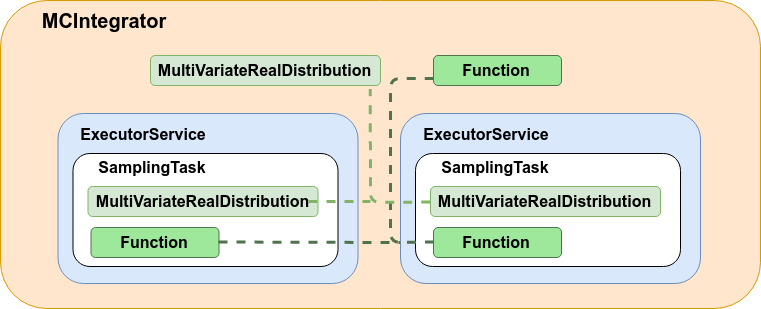
\includegraphics[width=.6\textwidth]{Chap5_DesignAndImplementation/MCIntegrator.png}
\caption{Instance diagram of an 2-thread MCIntegrator object, where the dashed lines denote copies of the same object}
\label{fig:MCIntegrator}
\end{center}
\end{figure}


\section{The \texttt{Solver} Package}
This package encapsulates the core software implementation of the Logistic Sampling algorithm. The classes implemented in this package fall into two main categories, with the exception of the \texttt{MonteCarloLogisticSolver} class which inherits from \texttt{QNSolver}:
\begin{itemize}
    \item Classes inheriting from the \texttt{LogisticFunctionBase} abstract class, which inherits from the \texttt{safeFunction} abstract class, and ultimately from the \texttt{Function} interface. These are implementations of the Integrand functions of the different versions of the Logistic Sampling algorithm. These are summarized in table \ref{table:logistic_function_class_names}. They contain methods to calculate the stationary point an hessian of the stationary point, and get them.
    \item Classes inheriting from the \texttt{LogisticCore} abstract class. \texttt{LogisticCore} is the main class that implements the Logistic Sampling algorithm, with the \texttt{LogisticCoreAdd} and \texttt{LogisticCoreMult} implementing the additive and multiplicative versions of the algorithm.
\end{itemize}

\begin{table}[!htb]
\begin{tabular}{@{}lll@{}}
\toprule
Transform type                  & Function Class Name               & Equation ref. \\ \midrule
\multirow{3}{*}{Additive}       & \texttt{LogisticFunction}         & Single-server network, eq (\ref{eq:log_integrand_single_server}) \\
                                & \texttt{LogisticFunctionDelay}    & Single-server network with delay, eq (\ref{eq:log_integrand_infinite_server})\\
                                & \texttt{LogisticFunctionMS}       & Multi-server network, eq (\ref{eq:log_integrand_multi_server_2})\\
\multirow{2}{*}{Multiplicative} & \texttt{LogisticFunctionMult}     & Single-server network, eq (\ref{eq:log_integrand_single_server_mult})\\
                                &  \texttt{LogisticFunctionMultDelay}  & Single-server network with delay, eq (\ref{eq:log_integrand_infinte_server_mult})\\ \bottomrule
\end{tabular}
\caption{Descriptions of Logistic Function}
\label{table:logistic_function_class_names}
\end{table}

\subsection*{\texttt{LogisticFunctionBase} and subclasses}

\texttt{LogisticFunctionBase} extends the \texttt{safeFunction} abstract class, by adding the following required (abstract) function declarations:
\begin{itemize}[noitemsep]
    \item \texttt{calculate\_stationary\_point}: function to call to calculate (and cache) the stationary point of the specified integrand
    \item \texttt{calculate\_hessian}: function to call to calculate (and cache) the stationary point of the specified integrand
    \item \texttt{getX\_stat}: get stationary point (in transformed domain) of the integrand
    \item \texttt{getHess\_stat}: get stationary point hessian (in transformed domain) of the integrand
\end{itemize}

All integrand functions inherit from \texttt{LogisticFunctionBase} and implement these methods.

Given that the \texttt{LogisticFunction} class inherits from the \texttt{safeFunction} abstract class, it implements its corresponding integrand function in abstract function \texttt{safeEvaluate}. Several design choices were made when implementing the \texttt{LogisticFunction} class, and its related classes:
\begin{itemize}
    \item Cached values include \(\eta_{\epsilon}(N) = N+K(1+\epsilon N)\) and \(\sigma_r = \sum_{k=K}^M \theta_{kr}\) , the latter being only for the \texttt{LogisticFunctionDelay} function. This is to save on a small amount of computation at each sample.
    \item For every class inheriting from the \texttt{LogisticFunctionBase} algorithm, \textit{except for} the \texttt{LogisticFunctionMS} (multiserver) class, the logistic integrand is first computed in terms of its logarithm \(h(\mathbf{x})\), in double precision. This is deemed enough for the logarithm, and has been robustly tested with numerous numerical experiments. The tensor multiplications are performed using the \texttt{DoubleMatrix1D} and \texttt{DoubleMatrix2D} classes from the \texttt{cern.colt} library. The computed log integrand is then raised to \(e^{-h(\mathbf{x})}\) in \texttt{BigDecimal} and returned.
    \item For the \texttt{LogisticFunctionMS} class, all arithmetic operations are performed with \texttt{BigDecimal}, with the specified precision.
    \item For the \texttt{LogisticFunctionMS} class, there is some overhead when enumerating the states and coefficients over which to apply the \(\boldsymbol{\Delta}\) operator in (\ref{eq:log_integrand_multi_server_2}). To save some computation, this is calculated at initialization, and cached. When applying the \(\boldsymbol{\Delta}\) and summation operators, we merely loop over these cached states, multiply by the cached coefficients, and result is summed.
\end{itemize}

For all of the above classes, the precision of the computation of the integrand can be specified by providing a \texttt{MathContext} object to the \texttt{LogisticFunction} class constructor with a specified precision in terms of the number of digits. All \texttt{BigDecimal} operations in the functions are calculated using the specified \texttt{MathContext}.

\subsection*{\texttt{LogisticCore} and subclasses}
The \texttt{LogisticCore} implements the core, higher-level structure of Logistic Sampling algorithm to calculate the normalizing constant, and the logic for distinguishing between the types for models (single-server only, single-server with delay, and multiserver). It is subclassed by the \texttt{LogisticCoreAdd} and \texttt{LogisticCoreMult} classes (for the additive and multiplicative version of the logistic sampling algorithms respectively). Each subclass will implement the \texttt{initialize\_logistic\_function()} which provides the correct version of the logistic function class.
\lstinputlisting[caption=\texttt{LogisticCoreAdd} implementation]{Chap5_DesignAndImplementation/LogisticCoreAdd.java}
\lstinputlisting[caption=\texttt{LogisticCoreMult} implementation]{Chap5_DesignAndImplementation/LogisticCoreMult.java}

\texttt{LogisticCore} then uses these logistic function implementations to calcluate and fetch the stationary point, and the hessian of the integrand at that point. It then finally uses these components to instantiate an \texttt{MCIntegrator} object to perform the integration. This is shown in full in the \texttt{LogisticCore} constructor shown below.
\lstinputlisting[caption=\texttt{LogisticCore} constructor implementation]{Chap5_DesignAndImplementation/LogisticCore.java}

To return the result of the Logistic Sampling algorithm, the public method \texttt{calculateNC()} returns a \texttt{BigDecimal} representing the result of the Monte Carlo Integration.

\subsection*{The Full Solver: \texttt{MonteCarloLogisticSolver}}
In order to provide an interface of the Logistic Core algorithm, the \texttt{MonteCarloLogisticSolver} solver subclass to the \texttt{QNSolver} was written. This class implements the pre-processing of the \texttt{QNModel} input into the solver, by extracting its demand matrix, delays, population vector, and server count. These are then used to check for an invalid model (negative demands, zero total demand for a station etc.). The solver is also responsible for computing and caching the model normalizing constant, and for the calculation of the performance indices (queue lengths and throughputs).
\\\\
To compute the performance indices, the solver has to calculate multiple normalizing constants, as the throughputs and queue lengths are expressed at the ratio of some modified normalizing (\(G'_{\boldsymbol{\theta}}(\mathbf{N})\)) over the true normalizing constant of the model (\(G_{\boldsymbol{\theta}}(\mathbf{N})\)). As a result, the solver instantiates multiple instances of a \texttt{LogisticCore} class, and inputs a modified model. For example the \texttt{augmentDemandsAtServer(int M, int R, DoubleMatrix2D demands, int k)} method is used to augment the model with a specified server \(k\). for the calculation of the queue-lengths at station \(k\).

\lstinputlisting[caption=\texttt{computePerformanceMeasures()} instantiation of multiple \texttt{LogisticCore} instances]{Chap5_DesignAndImplementation/MonteCarloLogisticPerfInd.java}

A full class diagram illustrating the relationships between the classes described above is shown in figure \ref{fig:DistributionsPackage}. 

\newpage
    \begin{figure}[H]
    \begin{center}
    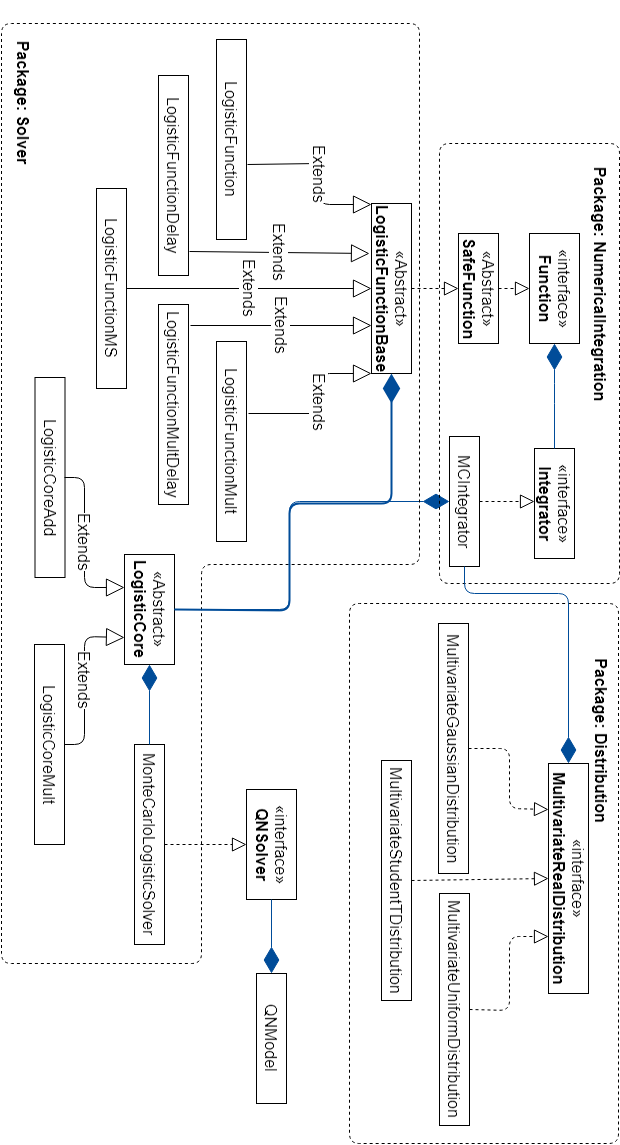
\includegraphics[width=.75\textwidth]{Chap5_DesignAndImplementation/DistributionsPackage.png}
    \caption{Package/class diagram of the implemented components within the \texttt{QueueingNet} framework}
    \label{fig:DistributionsPackage}
    \end{center}
    \end{figure}
\newpage

\section{Testing and Verification}
The modular design of the software has allowed the various components to be tested separately, making it easier to verify correctness for the subcomponents of the Logistic Sampling algorithm. Unit tests were mostly tested against reference implementations written in both MATLAB and python, for related projects, such as \cite{Casale2017AcceleratingMethods}. Unit tests were implemented to cover the following:
\begin{itemize}
    \item Testing the correctness of the implementations of the various distributions in \texttt{Distributions}. Simple example distributions were given, and samples were drawn from the distribution. For example, for the \texttt{MultivariateGaussian} distribution, a simple covariance structure was defined, and samples drawn from the corresponding zero-mean distribution. The maximum-likelihood covariance was computed and verified to be close to the original covariance by taking the matrix 2-norm:
    \[\frac{\Vert \hat{\Sigma}_{ML} - \Sigma \Vert}{\Vert \Sigma \Vert} < \epsilon   \]
    \item Testing the components of \texttt{NumericalIntegration} package. Simple implementations of the \texttt{Function} interface were made and used in conjunction with a simple distribution, in order to test the functionality of \texttt{MCIntegrator}. 
    \item Testing the correctness of the implementations of \texttt{LogisticFunctions} and related classes by checking against reference implementations, given fixed models and input points.
    \item The \texttt{LogisticCore} calculation of the normalizing constant was tested by comparing the log of the normalizing constant against an exact result. For small, simple models, given large enough \(N\), the errors were expected to fall below a reasonable threshold, e.g. \(\epsilon = 0.1\).
\end{itemize}

Ultimately, the true correctness of randomized algorithms can only be verified to a certain degree. The performance of the algorithm was again confirmed through repeated experimentation, which is covered extensively in the following chapters.

%%%%%%%%%%%%%%%%%%%%%%%%%%%%%%%%%%%%
\chapter{Evaluation and Analysis}\label{chap:EvalAnalysis} 

In this chapter, we turn our attention to the evaluation and analysis of the randomized integration of the normalizing constant \(G_{\boldsymbol{\theta}}(\mathbf{N})\), via the Logistic Sampling algorithm, introduced in chapters 3 and 4. Since we are analyzing approximate, randomized, methods, special attention is paid to error analysis. More specifically, we are interested in the distribution of what will be random errors, and the factors that effect this distribution. The results from the experiments will be discussed along with their relations to theoretical properties.

\section{Overview of Experiments}\label{sec:overview_experiments}
The aim of this section is to give an overview of the scope of the experiments, and the general methodologies which will be employed. 
\\\\
The experiments will involve testing the integration methods of the integral form of the normalizing constants (\ref{eq:integral_form_single_server}), (\ref{eq:integral_form_infinite_server}), (\ref{eq:integral_form_multi_server_1}), and (\ref{eq:integral_form_multi_server_2}). These all involve using the Monte Carlo Integration via the Logistic Sampling Algorithm to integrate a uni-modal integrand \(e^{-f(\mathbf{x})}\) by summing:
\[I \approx \frac{1}{N} \sum_{i=1}^N \frac{e^{-f(\mathbf{x_i})}}{p(\mathbf{x_i})}\]
Where \(\mathbf{x_i}\) is drawn from some candidate sampling distribution with probability density function \(p(\mathbf{x})\).
\\\\
Since we are concerned with the behaviour of random errors on the computed value of the normalizing constant, it is important to be able to have a ground truth to test against. These will usually be calculated from an exact algorithm for smaller models \(G_{EXACT}\). Exact algorithms used as a baseline include the Recursion by Chain (RECAL) algorithm, the Method-of-Moments(MoM) and the Mean-Value-Analysis (MVA) algorithms. The choice of exact algorithms are primarily based on speed of computation, depending the size of the model. We are primarily interested in the normalizing constant \(G\), the queue-lengths \(Q_{kr}\) of the model, as well as the throughputs \(\lambda_{r}\). The errors for each metric are calculated:
\[E(G) = \frac{G_{LS} - G_{EXACT}}{G_{EXACT}}\]
\[E(Q) = \frac{\sum_{kr} |Q_{kr,LS} - Q_{kr,EXACT}|}{\sum_{kr} Q_{EXACT}}\]
\[E(\lambda) = \frac{\sum_{r} |\lambda_{r,LS} - \lambda_{r,EXACT}|}{\sum_{r} \lambda_{EXACT}}\]

For larger models, exact analysis becomes computationally intractable, and Logistic Sampling with a much larger (\(>3\) orders of magnitude) number of samples is used instead. The use of Logistic Sampling with over \(10^3\) times more samples should minimally impact the expected errors of solutions with a smaller number of samples, since the expected impact will be at least 30 times smaller than expected errors (the logistic sampling algorithm is tested with a maximum of \(10^4\) samples, and the approximated exact solution will be computed with \(10^7\) samples).
\\\\
Across all experiments, the default settings for the Logistic Sampling algorithm are used:
\begin{itemize}
    \item the additive logistic transformation for the integrand function
    \item the t-distribution with degree of freedom \(\nu=4\) for sampling distribution
\end{itemize}

The only exception to this rule is section \ref{sec:Transforms_and_Distributions} where a different transform and different sampling distributions are experimented with. 
\\\\
The experiments performed are summarized as below:
\begin{itemize}
    \item Sections \ref{sec:analyze_model_variation} - \ref{sec:Transforms_and_Distributions} will test single server models only. 
    \item Section \ref{sec:analyze_model_variation} will explore the effect of varying the demands \(\boldsymbol{\theta}\) of the model, as well as the population class share in the population vector \(\mathbf{N}\), for fixed total population \(N\).
    \item Section \ref{sec:Analyze_K_R_N} will analyze the effect of increasing the dimensionality of the integration domain by increasing the number of nodes in the system \(K\), as well as other hyper-parameters such as the number of classes \(R\), and total population \(N\).
    \item Section \ref{sec:Transforms_and_Distributions} will explore the effect of using different techniques to carrying out Monte Carlo Integration, namely by changing the type of logistic transform, and sampling distributions. 
    \item In section \ref{sec:Analyze_Delays} and \ref{sec:Multiserver}, the errors on different types of networks will be examined in relation to the single-server node networks. In the case of multi-server networks, special attention is paid to the phenomenon of variance cancellation.
\end{itemize}

\subsection{Interpretation of Errors}
Given that the Logistic Sampling Algorithm is in essence a randomized method, careful interpretation of the errors is required. Since the computed answers are random, it is important to think about error values not as a constant value, but as a random variable, with an associated distribution.
\\\\
\textit{{\large Mean Absolute Error and Uncertainties}}
\\\\
As a primary measure of error, we would like to evaluate the mean absolute percentage error (MAPE, denoted \(M\)) over a number of evaluations. This is calculated:
\begin{empheq}[box=\mymath]{equation}
    M = \frac{1}{N} \sum_{i=1}^N |\epsilon_i| 
\end{empheq}
Where \(\epsilon_i\) is the error calculated at an evaluation \(i\):
\[\epsilon_i = \frac{G_i-G_{i,EXACT}}{G_{i,EXACT}}\]

Where \(N\) is the number of evaluations. Given any distribution of \(\epsilon_i\), the central limit theorem (CLT) tells us that:
\[\bar{M} \sim \mathcal{N} \bigg(M, \frac{\sigma^2}{N} \bigg)\]
Where \(\bar{M}\) is the estimated mean of the distribution of absolute errors \(|\epsilon_i|\), and \(M\) and \(\sigma\) are the exact means and variances of this distribution. \(N\) is the number of evaluated errors.

In the case of unknown variance \(\sigma\), however, we can instead use the sample variance \(S^2\) of \(|\epsilon_i|\):
\[S^2 = \frac{1}{N} \sum_{i=1}^N (|\epsilon_i| - \bar{M})^2\]

Given that we can only estimate the variance, we can expect the true MAPE, \(M\), to be distributed according to a t-distribution with degree of freedom \(\nu=N-1\), mean \(\mu = \bar{M}\) and scale \(\sigma = \frac{S}{\sqrt{N}}\):
\begin{empheq}[box=\mymath]{equation}
    M \sim t_{n-1}\bigg(\bar{M}, \frac{S}{\sqrt{N}} \bigg)
\end{empheq}

This gives us an idea of the spread of the error distribution. This can also be useful when we would like to take confidences on the estimated MAPE. We will frequently show the plots of the MAPE with errorbars of 95\% confidence interval, as this can give us a better idea of the undelying error distribution.
\\\\
Besides that, having a probability distribution on the MAPE, \(M\) will allow us to perform some hypothesis testing, especially when comparing the relative effectiveness of different techniques with respect to the estimated errors.
\\\\
\textit{{\large Modelling the Error Distribution as a Normal Distribution}}
\\\\
Since the normalizing constant computed by the logistic integration can be interpreted as a mean of a function \(\frac{f(\mathbf{x})}{p(\mathbf{x})}\), sampled over \(p(\mathbf{x})\):
\[ G = E_{p\mathbf{(x)}} \bigg[ \frac{f(\mathbf{x})}{p\mathbf{(x)}} \bigg]\]
\[ \epsilon = \frac{G - G_{EXACT}}{G_{EXACT}} \]

The by CLT, the distribution of \(\epsilon\) should be normally distributed as \(N \rightarrow \infty\), given a model \( \mathcal{M} \) and number of samples \(N\).
\[ \epsilon_{|N,\mathcal{M}} \sim \mathcal{N}(0, \sigma_{|\mathcal{M}}(N))\]

Besides that, as has been explained in section \ref{sec:MCI}, the error is expected to be a linear function of the square root of \(N\):
\[\sigma_{|\mathcal{M}}(N) \propto N^{-1/2}\]

Therefore, we can expect that, given a fixed model \(\mathcal{M}\), the errors would be normally distributed.
\\\\
In several experiments, however, we would like to evaluate the distribution of the error with respect to some standard distribution, for a set of random models. The normal distribution is good to be used as a baseline to asses the symmetricity, and the relative spread of the error distribution, relative to the shape of the gaussian. To do this, for each experiment of a set of random models, we will fit a maximum-likelihood gaussian distribution to the set of errors:
\[\hat{\mu}_{ML} = \frac{1}{N} \sum_{i=1}^N \epsilon_i \quad \hat{\sigma}_{ML} = \frac{1}{N}\sum_{i=1}^N (\epsilon_i - \hat{\mu}_{ML})^2\]

The Kolmogorov-Smirnov (KS) statistic will be used as a goodness-of-fit score. When the KS score is low, this means that the normal approximation is a good one. A high KS score indicates large deviations from a normal distribution. 
 

\section{Analyzing the Effect of Model Variation}\label{sec:analyze_model_variation}

\subsection{Specific Models}\label{sec:experiments_specific_models}

Analysis of the effect of model variation began by looking at specific models, with deliberately chosen demands \(\boldsymbol{\theta}\). The methodology is as follows: 
\begin{itemize}[noitemsep]
    \item Size of the models were fixed, by fixing the number of stations \(K\), and the number of classes \(R\) to \(K=R=2\).
    \item The population vector \(\mathbf{N}\) was fixed to be \([3,3]\)
    \item The demands for station 0 was fixed to be \(\theta_{00} = \theta_{01} = 1.\)
    \item The demands for station 1 was changed according to the table \ref{tab:specific_models_evaluate}, to simulate different loads on the servers.
    \item The number of integration samples was fixed to \(N=100\).
    \item 300 evaluations were performed per model, and the errors calculated at each evaluation. The RECAL algorithm was used as ground truth.
\end{itemize}

\begin{table}[H]
\begin{center}
\begin{tabular}{@{}lllll@{}}
\toprule
 Test Case &  \(\theta_{10}\) & \(\theta_{11}\) & Description \\ \midrule
 1 & \(0.\) & \(0.\) & Load only on station 0 \\
 2 & \(0.25\) & \(0.25\) & Light load on station 1, heavy load on station 0\\
 3 & \(1.\) & \(1.\) & Perfectly equal loads \\
 4 & \(4.\) & \(4.\) & Symmetric model to case 1, with heavy load on station 1 \\ \bottomrule
\end{tabular}
\end{center}
\caption{Models tested}
\label{tab:specific_models_evaluate}
\end{table} 

For each model, the estimated mean absolute percentage error (MAPE), denoted \(\bar{M}\) and its 95\% confidence intervals was calculated:

\begin{table}[H]
\begin{center}
\begin{tabular}{@{}llllll@{}}
\toprule
 Test Case & \(\bar{M} \%\) & \(\bar{M}\) \(95\%\) CI (+) & \(\bar{M}\) \(95\%\) CI (-) & \(\hat{\sigma}_{ML}\)\\ \midrule
    1 &\(3.05\) & \(2.77\) & \(3.33\) & \(3.85\) &  \\ 
    2 &\(2.71\) & \(2.48\) & \(2.93\) & \(3.36\) &  \\ 
    3 &\(0.794\) & \(0.721\) & \(0.867\) & \(1.02\) &  \\ 
    4 &\(2.65\) & \(2.41\) & \(2.88\) & \(3.34\) &  \\  \bottomrule
\end{tabular}
\end{center}
\caption{Model errors}
\label{tab:specific_models_error}
\end{table} 

A surprising result was the difference in error distributions than can be seen between case 3 and the other test cases, where errors were much lower than in the other cases. A quick look at the error histograms confirm this finding to be true. Besides that, the QQ plots show good conformity of the error distribution with its maximum likelihood normal distributions.

\begin{figure}[!htb]
\begin{center}
    \centering
    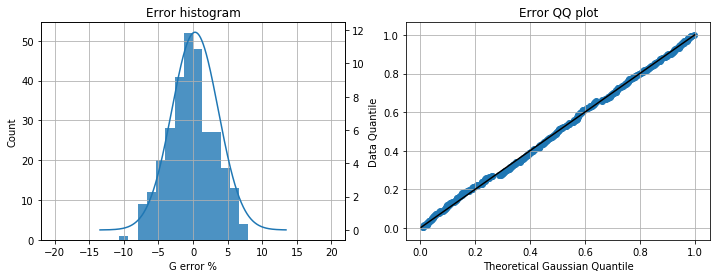
\includegraphics[width=1.0\textwidth]{Chap6_EvaluationAndAnalysis/images/Error_model_D_1_1_025_025_N_3_3.png}
\caption{Error distribution (fitted ML Gaussian in blue line) and QQ plot for case 2 -  \(\theta_{10}=\theta_{11}=0.25\)}
\label{fig:error_model_D_1_1_025_025_N_3_3}
\end{center}
\end{figure}

\begin{figure}[!htb]
\begin{center}
    \centering
    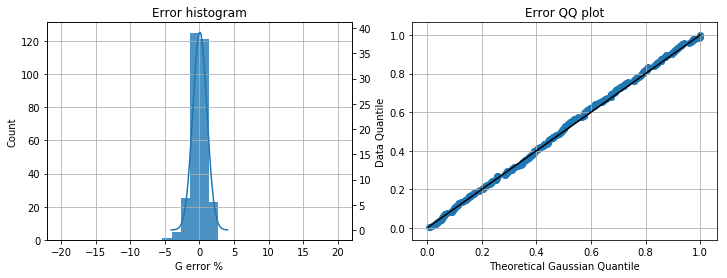
\includegraphics[width=1.0\textwidth]{Chap6_EvaluationAndAnalysis/images/Error_model_D_1_1_1_1_N_3_3.png}
\caption{Error distribution and QQ plot for case 3 - \(\theta_{10}=\theta_{11}=1\)}
\label{fig:error_model_D_1_1_1_1_N_3_3}
\end{center}
\end{figure}

When inspecting the shape of the integrand, one feature stood out for case 3 against all the remaining cases. The integrand was symmetric about its stationary point, as can be seen by comparing figure \ref{fig:spec_model_D_1_1_1_1_N_3_3} against figures \ref{fig:spec_model_D_1_1_0_0_N_3_3}, and \ref{fig:spec_model_D_1_1_4_4_N_3_3}.

\begin{figure}[!htb]
\begin{center}
\begin{subfigure}%[Simplex]
    \centering
    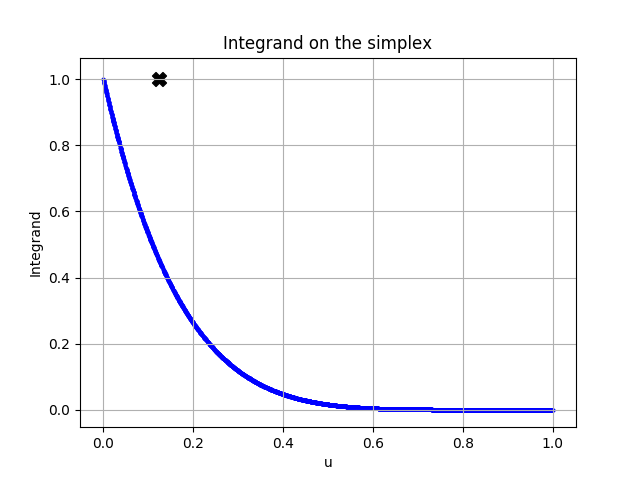
\includegraphics[height=2in]{Chap6_EvaluationAndAnalysis/images/Simplex_model_D_1_1_0_0_N_3_3.png}
\end{subfigure}
\begin{subfigure}%[Real]
    \centering
    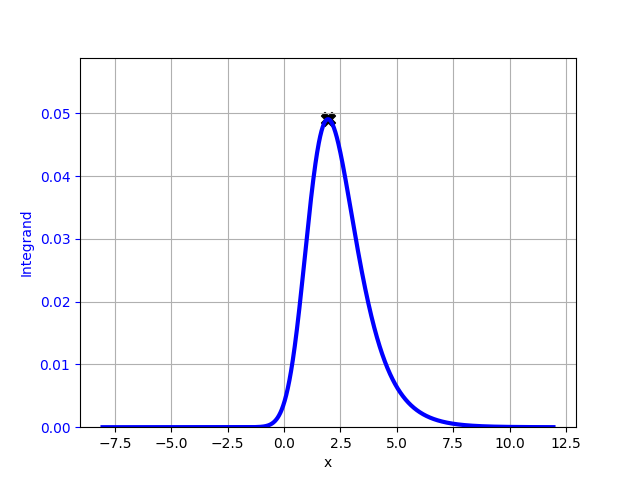
\includegraphics[height=2in]{Chap6_EvaluationAndAnalysis/images/Real_model_D_1_1_0_0_N_3_3.png}
\end{subfigure}
\caption{Test case 1 - \(\theta_{10}=\theta_{11}=0\). (Left) Shape of integrand on the simplex (Right) Shape of integrand after transform. Black cross in right plot represents stationary point of integrand function, and is re-projected back onto the simplex, shown in the left plot.}
\label{fig:spec_model_D_1_1_0_0_N_3_3}
\end{center}
\end{figure}

\begin{figure}[!htb]
\begin{center}
\begin{subfigure}%[Simplex]
    \centering
    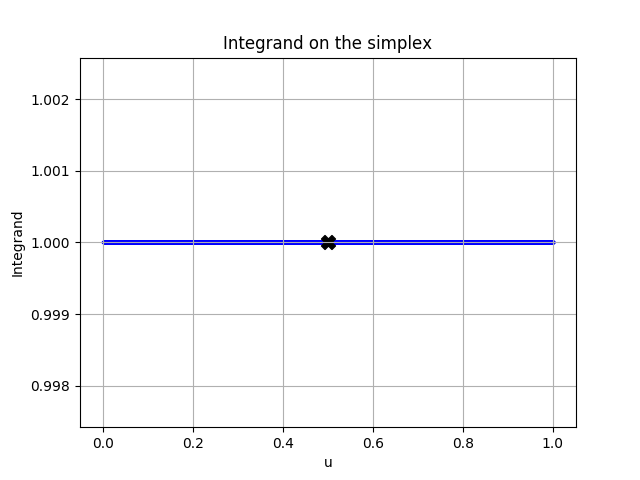
\includegraphics[height=2in]{Chap6_EvaluationAndAnalysis/images/Simplex_model_D_1_1_1_1_N_3_3.png}
\end{subfigure}
\begin{subfigure}%[Real]
    \centering
    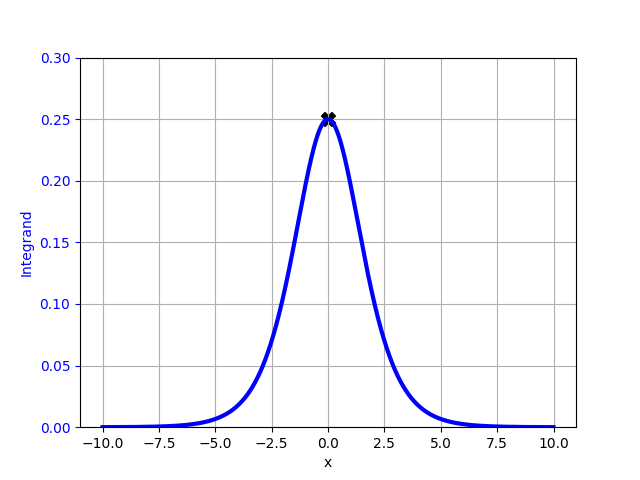
\includegraphics[height=2in]{Chap6_EvaluationAndAnalysis/images/Real_model_D_1_1_1_1_N_3_3.png}
\end{subfigure}
\caption{Test case 2 - \(\theta_{10}=\theta_{11}=1\)}
\label{fig:spec_model_D_1_1_1_1_N_3_3}
\end{center}
\end{figure}

 We can also inspect the shape of the distribution with respect to the integrand by overlaying the plot of the sampling distribution PDF of the model, and of the function to be integrated. It can be seen that the shape of the distribution in figure \ref{fig:sampling_pdfs_model}, for the left plot representing test case 2, the sampling distribution conforms much better with the integrand, while on the right plot which represents test case 3, the sampling distribution cannot capture the skewness of the integrand function. As discussed in section \ref{sec:MCI}, this would affect the contribution of the \(\frac{f(\mathbf{x})}{p(\mathbf{x})}\) term to the variance of the estimated integral \(\widetilde{I}\), and potentially lower the efficiency of the sampling. 
 
\begin{figure}[!htb]
\begin{center}
\begin{subfigure}%[Simplex]
    \centering
    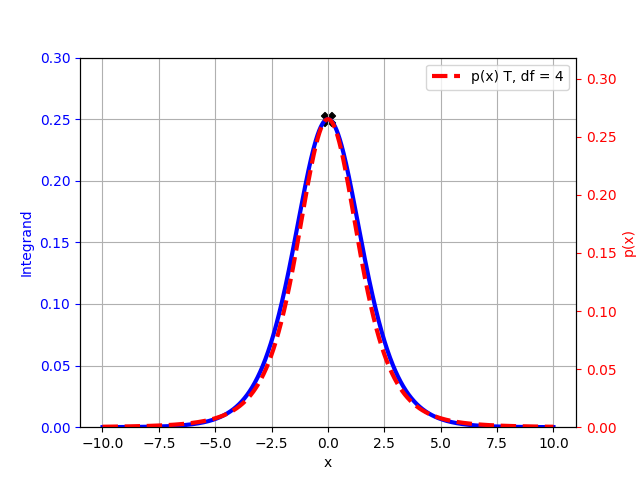
\includegraphics[height=2in]{Chap6_EvaluationAndAnalysis/images/px_D_1_1_1_1_N_3_3.png}
\end{subfigure}
\begin{subfigure}%[Real]
    \centering
    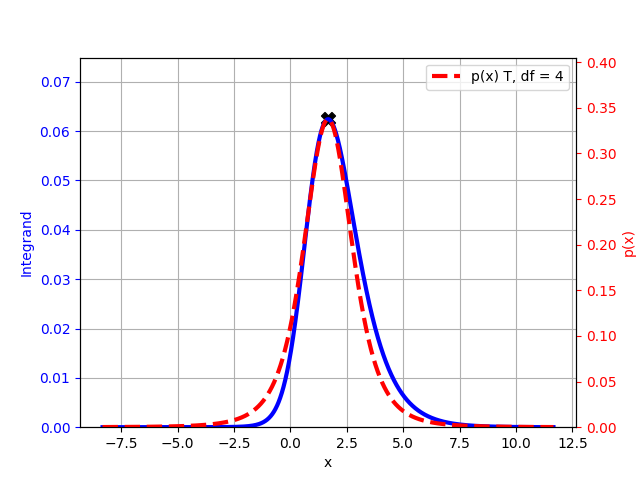
\includegraphics[height=2in]{Chap6_EvaluationAndAnalysis/images/px_D_1_1_025_025_N_3_3.png}
\end{subfigure}
\caption{Integrand (blue) overlaid with sampling distribution (red): Test Case 2 (Left) \(\theta_{10}=\theta_{11}=1\), Test Case 3 (Right) \(\theta_{10}=\theta_{11}=0.25\)}
\label{fig:sampling_pdfs_model}
\end{center}
\end{figure}

\begin{figure}[!htb]
\begin{center}
\begin{subfigure}%[Simplex]
    \centering
    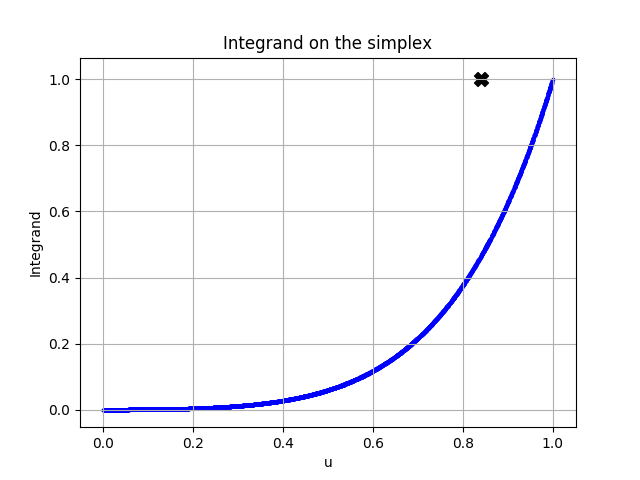
\includegraphics[height=2in]{Chap6_EvaluationAndAnalysis/images/Simplex_model_D_1_1_4_4_N_3_3.png}
\end{subfigure}
\begin{subfigure}%[Real]
    \centering
    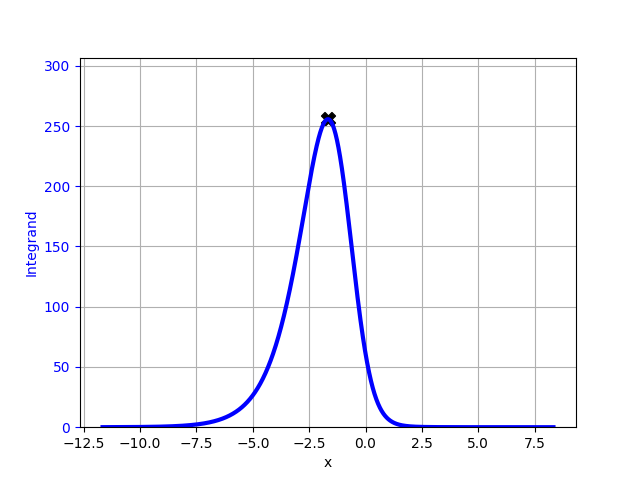
\includegraphics[height=2in]{Chap6_EvaluationAndAnalysis/images/Real_model_D_1_1_4_4_N_3_3.png}
\end{subfigure}
\begin{subfigure}%[Simplex]
    \centering
    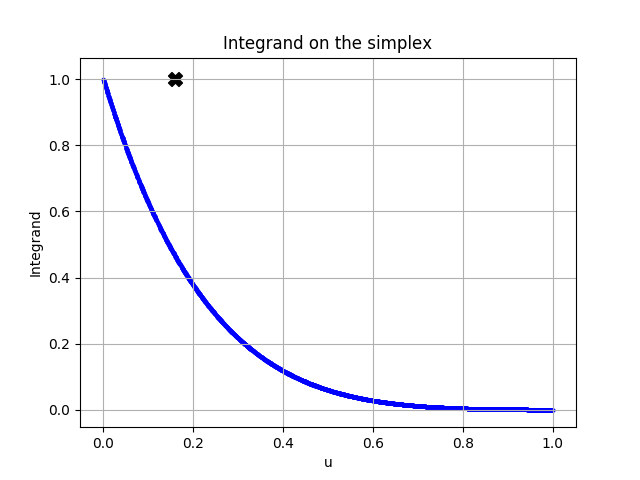
\includegraphics[height=2in]{Chap6_EvaluationAndAnalysis/images/Simplex_model_D_1_1_025_025_N_3_3.png}
\end{subfigure}
\begin{subfigure}%[Real]
    \centering
    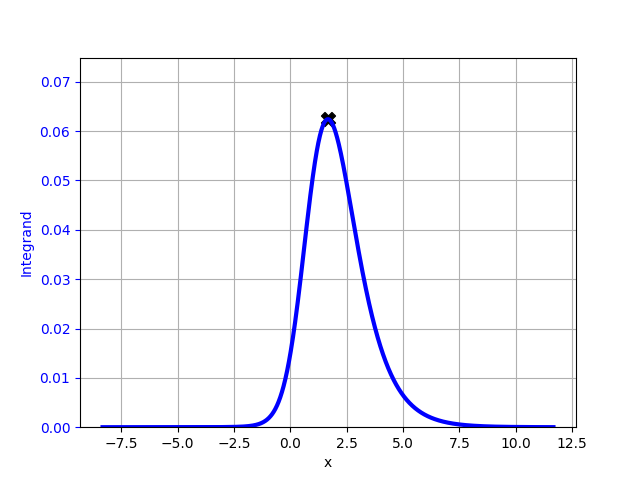
\includegraphics[height=2in]{Chap6_EvaluationAndAnalysis/images/Real_model_D_1_1_025_025_N_3_3.png}
\end{subfigure}
\caption{Test case 3 - (top) \(\theta_{10}=\theta_{11}=0.25\), Test case 4 - (bottom) \(\theta_{10}=\theta_{11}=4\)}
\label{fig:spec_model_D_1_1_4_4_N_3_3}
\end{center}
\end{figure}

\subsection{Relating Stationary Point Location with Expected Errors}

It was believed that one source of the skewness observed in the previous section's test cases was due to the location of the stationary point in the simplex. The shape of functions with skewed stationary points tend to more skewed on the simplex, this is also further magnified by the effect of the Jacobian which is a concave function on the simplex, and introduces a sharper gradient on the function about its stationary point, for skewed stationary points on the simplex, giving it asymmetry.
\\\\
In order to investigate this, a similar experiment to the one in section \ref{sec:experiments_specific_models} was performed. However, instead of hand-picking 4 models to evaluate, \(60 \times 60\) models were evaluated. Models with \(K=R=2\) were tested. \(60\) evenly spaced values each of \(\theta_{10}\) and \(\theta_{11}\), between \(\theta=0.0\) and \(\theta=4.0\). At each value of the \((\theta_{10}, \theta_{11})\) pair, 20 evaluations of the normalizing constant were performed, and a MAPE value was calculated.
\\\\
3 experiments were conducted with the above setup. In each experiment, the population vector was changed. For \(N=6\), 3 population shares were investigated: \(\mathbf{N} = [3,3]\), \(\mathbf{N} = [2,4]\), \(\mathbf{N} = [1,5]\). 
\\\\
Since we are trying to find out if stationary point deviation from the centre of the simplex affects the error of the model calculation, we seek to identify models with stationary points satisfying the following relation (where \(\mathbf{\hat{u}}\) is the stationary point of the model):
\[\hat{u}_0 = \hat{u}_1 = ... = \hat{u}_K = 1/K\]

For the 2 station case (\(K=2\)), given a population vector \(\mathbf{N} = [N_0, N_1]\), the stationary point equations become (for \(i = 1,2\)):
\[0.5 = \eta^{-1}(N) \bigg( 1 + 0.5 \sum_{r=1}^R \xi_r(\mathbf{\hat{u}}) \theta_{ir} \bigg)\]
Where \( \xi_r(\mathbf{\hat{u}}) = 0.5 N_r (\sum_{k=1}^K \theta_{kr})\)
\\\\
In all three experiments, demands for station 1 was set to 1. for all classes \(\theta_{00} = \theta_{01} = 1.\) The system of equations reduces to:
\[ \theta_{00} \xi_0 + \theta_{01} \xi_1 = \theta_{10} \xi_0 + \theta_{11} \xi_1\]

Using the definition of \(\xi_0, \xi_1\) and the fact that \(\theta_{00} = \theta_{01} = 1.\), the equation reduces to:
\begin{empheq}[box=\mymath]{equation}
    \label{eq:centre of simplex models}
    \frac{N_0}{1 + \theta_{10}} + \frac{N_1}{1 + \theta_{11}} = \frac{N_0 \theta_{10}}{1 + \theta_{10}} + \frac{N_1 \theta_{11}}{1 + \theta_{11}}
\end{empheq}
Therefore, the models of interest have \(\theta_{10}\) and \(\theta_{11}\) which satisfy the above equation.
\\\\
\textit{{\large Test Case 1: \(\mathbf{N} = [3,3]\)}}\\
In the first case, the population vector was set to \((3,3)\). When \(N_0 = N_1 = N\), the equation (\ref{eq:centre of simplex models}) simplifies to become:
\begin{empheq}[box=\mymathtwo]{equation*}
    \theta_{10} = \frac{1}{\theta_{11}}
\end{empheq}


The color in figure \ref{fig:bottleneck_analysis_balanced_pop} shows the distribution of errors, with the color scale shown on the right. The region of lowest error corresponds to the region around the line \(y = 1/x\), which represent models having stationary points at the centre of the simplex. \\

\begin{figure}[!htb]
\begin{center}
    \centering
    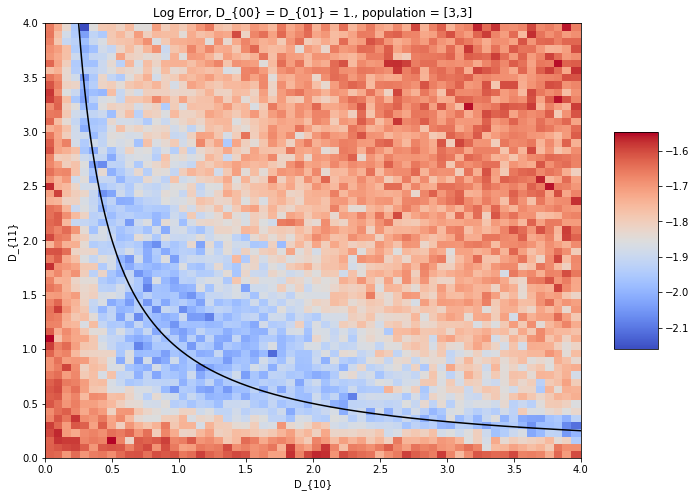
\includegraphics[width=0.8\textwidth]{Chap6_EvaluationAndAnalysis/images/error_analysis_bottleneck_balanced_pop.png}
\caption{Error plot for models and population \(\mathbf{N}=[3,3]\)}
\label{fig:bottleneck_analysis_balanced_pop}
\end{center}
\end{figure}

This does not seem to have any relation with the notion of a 'bottleneck' station. For the above model with the specified population, the line of constant load for station 1 is: 
\[\theta_{10} + \theta_{11} = C\]

Where \(C\) is a constant denoting the relative load on the second station. When \(C=2\), the load is balanced between station 0 and station 1. When \(C>2\), station 1 is more heavily loaded, and when \(C<2\), station 0 is more heavily loaded. However, it can be seen that lines of constant \(C\) to not correspond to lines of constant error. 
\\\\
\textit{{\large Test Case 2: \(\mathbf{N} = [2,4]\)}}
\\
The error color plot for this is shown in figure \ref{fig:bottleneck_analysis_pop_24}. When the population vector is set to \(\mathbf{N} = [2,4]\), the centre-of-simplex equations becomes:
\begin{empheq}[box=\mymathtwo]{equation*} \theta_{11}(3 \theta_{10} - 1) = 3 - \theta_{10} \end{empheq}
Again, the line of minimum error \(y = (3 - x)/(3x - 1)\) is plotted in black against the error color plot.\\\\

\begin{figure}[!htb]
\begin{center}
    \centering
    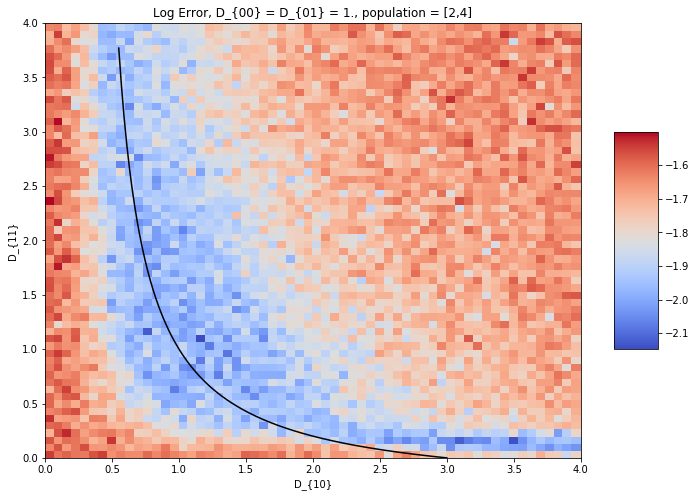
\includegraphics[width=0.8\textwidth]{Chap6_EvaluationAndAnalysis/images/error_analysis_bottleneck_pop_24.png}
\caption{Error plot for models and population \(\mathbf{N}=[2,4]\)}
\label{fig:bottleneck_analysis_pop_24}
\end{center}
\end{figure}

\textit{{\large Test Case 3: \(\mathbf{N} = [5,1]\)}}\\

\begin{figure}[!htb]
\begin{center}
    \centering
    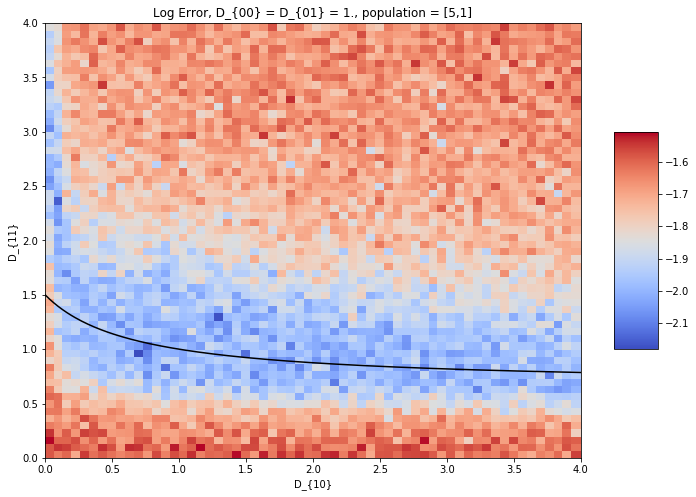
\includegraphics[width=0.8\textwidth]{Chap6_EvaluationAndAnalysis/images/error_analysis_bottleneck_pop_51.png}
\caption{Error plot for models and population \(\mathbf{N}=[5,1]\)}
\label{fig:bottleneck_analysis_pop_51}
\end{center}
\end{figure}

The error color plot for this is shown in figure \ref{fig:bottleneck_analysis_pop_51}. When the population vector is set to \(\mathbf{N} = [5,1]\), equation \ref{eq:centre of simplex models} becomes:
\begin{empheq}[box=\mymathtwo]{equation*} \theta_{11}(3 \theta_{10} + 2) = 3 + 2 \theta_{10} \end{empheq}
This gives us the black line of minimum error as shown in figure \ref{fig:bottleneck_analysis_pop_51}. 
\\\\
It is also quite interesting to plot the MAPE of the normalizing constant estimate, against distance of a model's stationary point from the centre of a simplex. The plot in figure \ref{fig:MAPE_vs_uhat} shows good correlation between the two quantities.
\begin{figure}[!htb]
\begin{center}
    \centering
    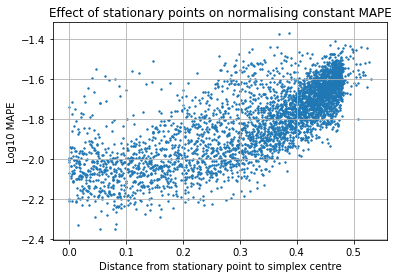
\includegraphics[width=0.8\textwidth]{Chap6_EvaluationAndAnalysis/images/NC_error_vs_uhat.png}
\caption{Plot of \(\log_{10}(MAPE)\) against distance of \(\mathbf{\hat{u}}\) from centre of simplex}
\label{fig:MAPE_vs_uhat}
\end{center}
\end{figure}

In conclusion, in general, there does not seem to be any correlation with the physical notion of the 'loading' of certain stations, and calculation errors of the normalizing constant. The shape of the integrand has a much larger part to play in the error estimate of the model, since this is a dominating factor in the efficiency of Monte Carlo Sampling, and by extension the Logistic Sampling algorithm. Although by no means a strict rule, it seems to be the general trend that a well-centered model on the simplex tends to be more accurately calculated. These are models which satisfy the following equation:

\[K^{-1} = \eta^{-1}(N) \bigg( 1 + \sum_{r=1}^R \frac{N_r \theta_{ir}}{\sum_k^K \theta_{kr} } \bigg)\]

\section{Effects of Number of Classes, Servers, and Populations}\label{sec:Analyze_K_R_N}
In this section, we will try to analyze the error distribution with respect to the size of the model. We begin first by looking at the convergence behaviour of errors with respect to the number of integration samples \(n_s\). Next we will observe the behaviour of errors with respect to number of classes, population, and finally the number of stations.
\\\\
Two experiments were conducted for the error analysis: 
\begin{itemize}[noitemsep]
    \item A set of small models where \(K,R \in [2,4,6]\) , and a set of medium-large models where \(K,R \in [8,12,16]\) were tested.
    \item For each combination of \(K\) and \(R\), 100 randomized models were tested, where \(\theta\) was sampled uniformly. Hence the effect of a model \(\mathcal{M}\) was marginalized out.
    \item For each model the population was ramndomized, where each class population \(N_r \sim \mathcal{U}(1,5)\). 
    \item Each model was tested with a different number of samples, ranging from \(10^1\) to \(10^4\).
\end{itemize}

\subsection{Initial look at Convergence}
An initial look at the convergence plots for small models (\(K,R \in [2,4,6]\)) shows that Monte Carlo Integration theory is right: that the estimated error is square-root convergent. The tabulated errors in table \ref{tab:convergence_tabulated_errors} show the MAPE for the normalizing constant (denoted \(\bar{M}(G)\)), the queue-lengths (\(\bar{M}(Q)\)) and throughputs (\(\bar{M}(\lambda)\)), averaged over all \(3 \times 3 \times 100\) models. The max-likelihood estimate of the \(G\) standard error is denoted \(\hat{\sigma}(G)\). The KS score is also shown, indicating slight deviation from normality, given that a variety of models of different sizes are considered.
\\\\
Furthermore, figure \ref{fig:OverallConvergence} on the right plots the log (base 10) of estimated MAPE values against the number of samples on a log scale. The gradients of these plots can be seen to be almost exactly \(1/2\). These values are again plotted on the right figure \ref{fig:OverallConvergence} alongside errorbars representing the 95\% confidence interval of the true value of the MAPE. The MAPE for Queue Length and Throughputs can be seen to be slightly higher on average since they involve computing more than 1 value of a normalizing constant.

\begin{table}[H] 
\begin{center}
\begin{tabular}{@{}lllllll@{}}
\toprule
    \(N\) & KS score & \(\bar{M}(G)\) \% & \(\hat{\sigma}(G)\) \% & \(\bar{M}(Q)\) \% & \(\bar{M}(\lambda)\) \% \\  \midrule
    10 &\(0.091\) & \(14.979\) & \(20.834\) & \(26.782\) & \(22.251\) &  \\ 
    20 &\(0.115\) & \(11.413\) & \(17.019\) & \(18.079\) & \(16.251\) &  \\ 
    50 &\(0.102\) & \(6.948\) & \(10.214\) & \(11.713\) & \(9.717\) &  \\ 
    100 &\(0.098\) & \(5.077\) & \(7.300\) & \(8.515\) & \(7.123\) &  \\ 
    200 &\(0.093\) & \(3.636\) & \(5.239\) & \(6.395\) & \(5.185\) &  \\ 
    500 &\(0.096\) & \(2.272\) & \(3.241\) & \(3.942\) & \(3.322\) &  \\ 
    1000 &\(0.095\) & \(1.743\) & \(2.507\) & \(2.759\) & \(2.478\) &  \\ 
    2000 &\(0.086\) & \(1.198\) & \(1.693\) & \(1.940\) & \(1.690\) &  \\ 
    5000 &\(0.085\) & \(0.782\) & \(1.120\) & \(1.255\) & \(1.075\) &  \\ 
    10000 &\(0.080\) & \(0.526\) & \(0.751\) & \(0.860\) & \(0.745\) &  \\     \bottomrule
\end{tabular}
\end{center}
\caption{Tabulated Mean Absolute Percentage Error(MAPE, denoted \(E\)) and standard errors denoted \(\sigma\), for small models \(K,R \in [2,4,6]\)}
\label{tab:convergence_tabulated_errors}
\end{table} 

\begin{figure}[!htb]
\begin{center}
\begin{subfigure}
    \centering
    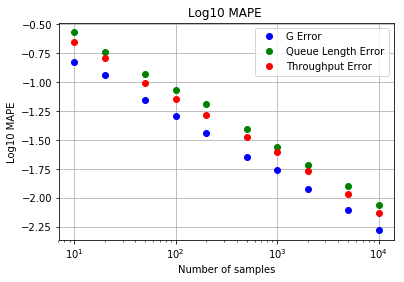
\includegraphics[width=0.45\textwidth]{Chap6_EvaluationAndAnalysis/images/OverallConvergence.png}
\end{subfigure}
\begin{subfigure}
    \centering
    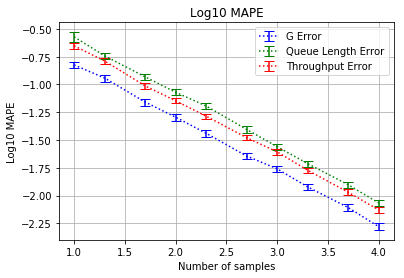
\includegraphics[width=0.45\textwidth]{Chap6_EvaluationAndAnalysis/images/OverallConvergenceSigma.png}
\end{subfigure}
\caption{(Left) Convergence plot for log10 MAPE, (Right) with 95\% CI errorbars}
\label{fig:OverallConvergence}
\end{center}
\end{figure}

\begin{figure}[!htb]
\begin{center}
    \centering
    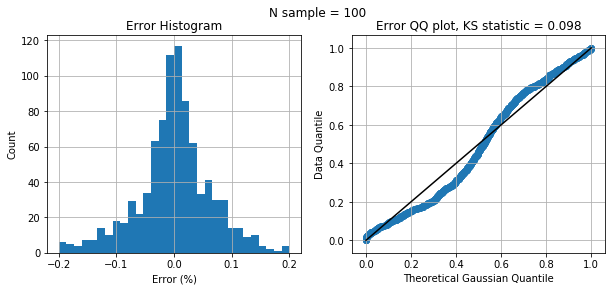
\includegraphics[width=0.8\textwidth]{Chap6_EvaluationAndAnalysis/images/N100_KR246.png}    
\caption{Error histogram (Left) and QQ plot (Right) of the errors vs. its Max Likelihood Gaussian for all small models (\(K,R \in [2,4,6]\)), and number of smaples = \(100\), shown with its Kolmogorov-Smirnov statistic. Both the KS statistic and QQ plots indicate slight divergence from normality}
\label{fig:ErrorHistN100_KR246}
\end{center}
\end{figure}

\subsection{Varying model size and population}

Separating the datasets by number of classes and plotting a convergence plot, we see quite clearly that the error distribution for the models hardly depends on the number of classes of customers in the model. This is a very good property to have, since we can scale the number of classes in the model up, without having to worry about increasing errors.

\begin{figure}[!htb]
\begin{center}
\begin{subfigure}
    \centering
    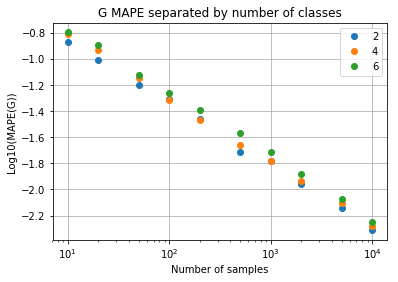
\includegraphics[width=0.45\textwidth]{Chap6_EvaluationAndAnalysis/images/ConvergenceNumberOfClasses_SM_meanerr.png}
\end{subfigure}
\begin{subfigure}
    \centering
    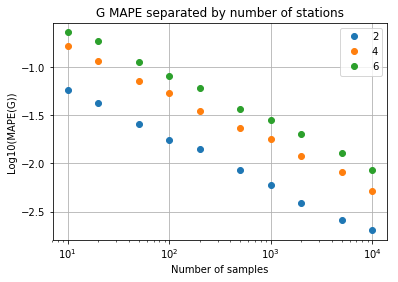
\includegraphics[width=0.45\textwidth]{Chap6_EvaluationAndAnalysis/images/ConvergenceNumberOfStations_SM_meanerr.png}
\end{subfigure}
\caption{Convergence plot for the MAPE of normalizing constant \(\bar{M}(G)\), separated by number of classes (left) ,and number of stations (right)}
\label{fig:ClassSeparatedConvergence_MAPE}
\end{center}
\end{figure}

\begin{figure}[!htb]
\begin{center}
\begin{subfigure}
    \centering
    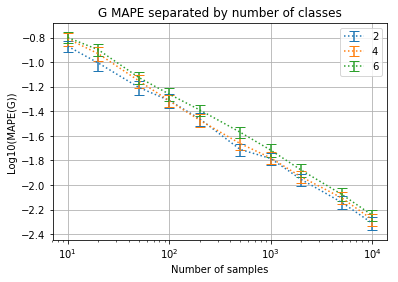
\includegraphics[width=0.45\textwidth]{Chap6_EvaluationAndAnalysis/images/ConvergenceNumberOfClasses_SM.png}
\end{subfigure}
\begin{subfigure}
    \centering
    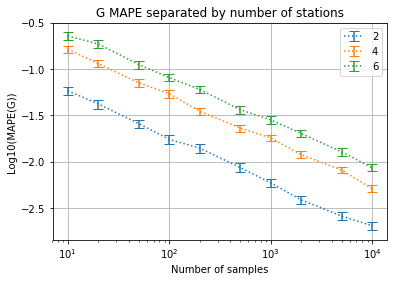
\includegraphics[width=0.45\textwidth]{Chap6_EvaluationAndAnalysis/images/ConvergenceNumberOfStations_SM.png}
\end{subfigure}
\caption{Convergence plot for the MAPE of normalizing constant \(\bar{M}(G)\) for small models, errorbars are \(95\%\) CI from t-distribution of the true MAPE}
\label{fig:ClassSeparatedConvergence}
\end{center}
\end{figure}


The number of stations, on the other hand, has quite a significant effect on \(\bar{M}(G)\). This is understandable since the number of dimensions to integrate over is larger, we would expect a larger starting error. Note that this does not, however, impact the convergence of errors with respect to the number of samples.
\\\\
\textit{{\large Medium-Large Models \(K,R = [8,12,16]\)}}
\\\\
The results for small models also seem to extend to large models. However, for large models, the ground truth was not available due to time constraints, since it would take far too long for exact calculations of the normalizing constant to complete. For each model, Logistic Sampling with \(10^7\) samples was used to estimate the ground truth, guaranteeing that errors introduced would be \textit{at least} \(30\) times smaller on average.
\\\\
Besides that, it was observed that for larger models, mixing models of different sizes which have quite different error distributions, can produce a highly non-normal distribution, since the assumption of independence of error on the number of stations is shown to be a poor one. This is reflected in the KS score shown in the table below. The estimate of the MAPE for larger models is shown to have a larger spread as well (shown by the error bars), especially for tests with a smaller number of samples. This uncertainty could possibly be due to the use of an approximation for \(G_{EXACT}\).

\begin{table}[H] 
\begin{center}
\begin{tabular}{@{}llll@{}}
\toprule
    \(N\) & KS score & \(\bar{M}(G)\)  & \(\hat{\sigma}_{ML}(G)\) \\  \midrule
    10 &\(0.262\) & \(0.491\) & \(1.337\) \\ 
    20 &\(0.152\) & \(0.361\) & \(0.596\)  \\ 
    50 &\(0.275\) & \(0.278\) & \(0.911\)  \\ 
    100 &\(0.176\) & \(0.199\) & \(0.424\)  \\ 
    200 &\(0.137\) & \(0.151\) & \(0.242\)  \\ 
    500 &\(0.081\) & \(0.098\) & \(0.134\) \\ 
    1000 &\(0.126\) & \(0.082\) & \(0.134\) \\ 
    2000 &\(0.171\) & \(0.056\) & \(0.111\) \\ 
    5000 &\(0.108\) & \(0.036\) & \(0.054\) \\ 
    10000 &\(0.065\) & \(0.026\) & \(0.037\)  \\     \bottomrule
\end{tabular}
\end{center}
\caption{Tabulated Mean Absolute Percentage Error, for large models \(K,R \in [8, 12, 16]\)}
\label{tab:convergence_tabulated_errors_LM}
\end{table} 

The plot of the MAPE of the normalizing constant (\(\bar{M}(G)\)) with confidence intervals for large models are shown in figures \ref{fig:ClassSeparatedConvergence_LM}, separated by classes and stations respectively:

\begin{figure}[!htb]
\begin{center}
\begin{subfigure}
    \centering
    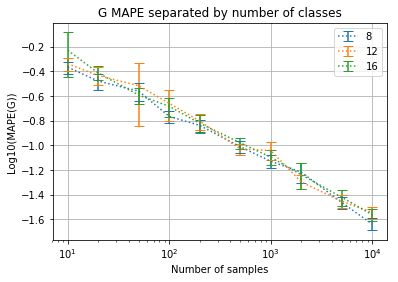
\includegraphics[width=0.45\textwidth]{Chap6_EvaluationAndAnalysis/images/ConvergenceNumberOfClasses_LM.png}
\end{subfigure}
\begin{subfigure}
    \centering
    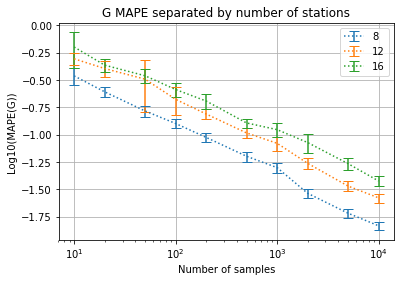
\includegraphics[width=0.45\textwidth]{Chap6_EvaluationAndAnalysis/images/ConvergenceNumberOfStations_LM.png}
\end{subfigure}
\caption{Convergence plot for large models, separated by number of classes and stations.}
\label{fig:ClassSeparatedConvergence_LM}
\end{center}
\end{figure}

The same values are shown in figure \ref{fig:ClassSeparatedConvergence_LM_meanerr} without its 95 \% confidence intervals:

\begin{figure}[!htb]
\begin{center}
\begin{subfigure}
    \centering
    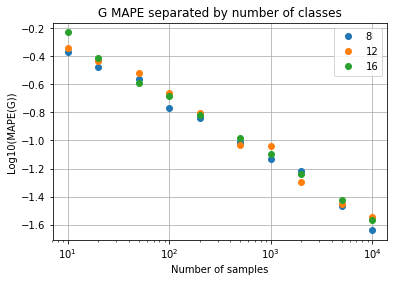
\includegraphics[width=0.45\textwidth]{Chap6_EvaluationAndAnalysis/images/ConvergenceNumberOfClasses_LM_meanerr.png}
\end{subfigure}
\begin{subfigure}
    \centering
    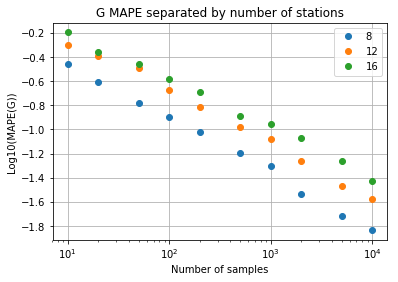
\includegraphics[width=0.45\textwidth]{Chap6_EvaluationAndAnalysis/images/ConvergenceNumberOfStations_LM_meanerr.png}
\end{subfigure}
\caption{Convergence plot for large models, separated by number of classes and stations.}
\label{fig:ClassSeparatedConvergence_LM_meanerr}
\end{center}
\end{figure}

\section{Effects of Transforms and Sampling Distribution}\label{sec:Transforms_and_Distributions}

For this section we analyze the behaviour of the normalizing constant error \(\epsilon\) when integration sampling distribution (gaussian or student-t), and the type of logistic transform (additive or multiplicative) is changed. When performing a comparison, models with the same number of stations and classes are considered in isolation, in order to remove the effect the model size has on the error distribution, since errors can have strong dependence on the model size. This allows us to perform a better analysis of the errors. The (number of station, number of classes) \((K,R)\) pairs tested were : \((2,2), (4,4), (6,6)\)

\subsection{Choice of Sampling Distribution}

For all 3 cases : \((K=R=2)\), \((K=R=4)\), \((K=R=6)\), the results were very similar qualitatively. Here we will present plots and figures for the case \(K=R=6\). Tables for \(K=R=2\) and \(K=R=4\) are provided in appendix \ref{app:extra_experiments}. The transform used was the additive logistic transform.
\\\\
\textit{{\large Multivariate Gaussian Sampling Distribution}}
\\\\
In this comparison, two types of sampling distributions were considered: the Multivariate Gaussian, and the Multivariate Student-t distribution. The shapes of these distributions can approximate the shape of the integrand well by using the Hessian \(\mathbf{A}\) at the stationary point \(\mathbf{\hat{x}}\) as the covariance matrix \(\boldsymbol{\Sigma} = \mathbf{A}^{-1}\).
\\\\
In the case of the Multivariate Gaussian, a slight change was made: a scaling factor \(s\) was introduced to the covariance matrix \(\boldsymbol{\Sigma} = s\mathbf{A}^{-1}\). This allows the multivariate Gaussian to sample from a larger area in the region around the integrand mode. 
\\\\
\begin{figure}[!htb]
\begin{center}
\begin{subfigure}
    \centering
    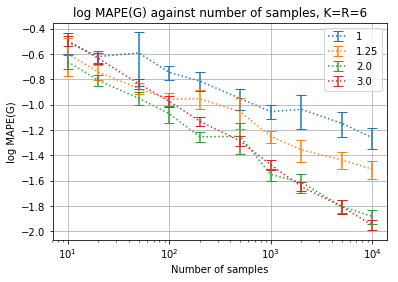
\includegraphics[width=0.45\textwidth]{Chap6_EvaluationAndAnalysis/distribution_variation/Convergence_scale_KR6_gaussian.png}
\end{subfigure}
\begin{subfigure}
    \centering
    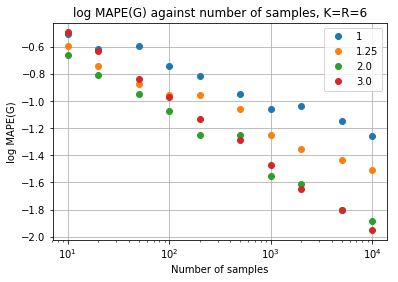
\includegraphics[width=0.45\textwidth]{Chap6_EvaluationAndAnalysis/distribution_variation/Convergence_scale_KR6_gaussian_meanerr.png}
\end{subfigure}
\caption{Convergence plot for \(K=R=6\) models, when integrated using different scales \(s\) for the Gaussian Covariance. On the left is a plot of the log of MAPE , with \(95\%\) confidence intervals. The MAPE estimate is on the right without errorbars}
\label{fig:ConvergencePlotGaussianScales}
\end{center}
\end{figure}

It can be seen in the MAPE convergence plot \ref{fig:ConvergencePlotGaussianScales} that for smaller values of \(s\), the error statistics are more noisy. Besides that, on average, the MAPE values are higher. As \(s\) increases, the plots becomes less noisy, and errors decrease on average. A quick inspection of the error histograms shows why this is the case:

\begin{figure}[!htb]
\begin{center}
    \centering
    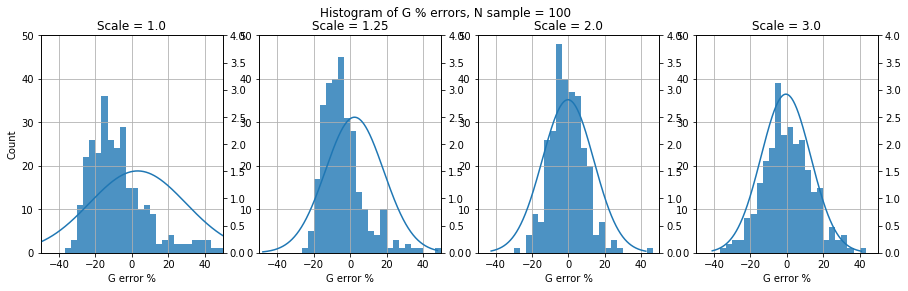
\includegraphics[width=1.0\textwidth]{Chap6_EvaluationAndAnalysis/distribution_variation/hist_KR6_gaussian.png}    
\caption{Error histograms of the errors vs. its Max Likelihood Gaussian for models where \(K=R=6\), and number of samples = \(100\), and different scales \(s\)}
\label{fig:hist_KR6_gaussian}
\end{center}
\end{figure}

\begin{figure}[!htb]
\begin{center}
    \centering
    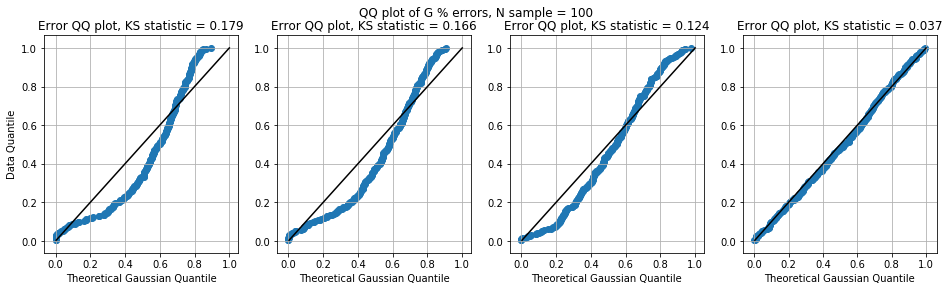
\includegraphics[width=1.0\textwidth]{Chap6_EvaluationAndAnalysis/distribution_variation/QQ_KR6_gaussian.png}
\caption{QQ plot of the errors vs. its Max Likelihood Gaussian for models where \(K=R=6\), and number of samples = \(100\), with different scales \(s\).}
\label{fig:QQ_KR6_gaussian}
\end{center}
\end{figure}

We can observe from figures \ref{fig:hist_KR6_gaussian} and \ref{fig:QQ_KR6_gaussian} that for smaller values of \(s\), not only the error distribution is poorly approximated by a normal distribution, but that the error of \(G\) is negatively biased - i.e. the Logistic Sampling algorithm has a tendency to underestimate the normalizing constant. Besides that, the error distributions for smaller \(s\) have heavier tails, indicating many outliers, which explains the noisiness in the mean error. As \(s\) is increased, the error distribution approaches the normal distribution, and the bias disappears.
\\\\
\textit{{\large Multivariate Student-t Sampling Distribution}}
\\\\
Next the Logistic Sampling algorithm was tested with the student-t distribution as the integration sampling distribution. Similarly to the multivariate Gaussian, the covariance parameter \(\boldsymbol{\Sigma}\) here used was the inverse of the Hessian of the logistic integrand. The experiments here involved changing the degree-of-freedom (DOF) parameter of the t-distribution (denoted \(\nu\)), and observing its error distribution.
\\\\
\begin{figure}[!htb]
\begin{center}
\begin{subfigure}
    \centering
    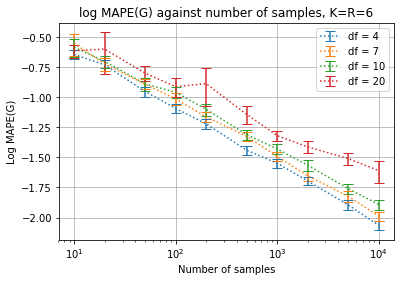
\includegraphics[width=0.45\textwidth]{Chap6_EvaluationAndAnalysis/distribution_variation/Convergence_DF_KR6_tdist.png}
\end{subfigure}
\begin{subfigure}
    \centering
    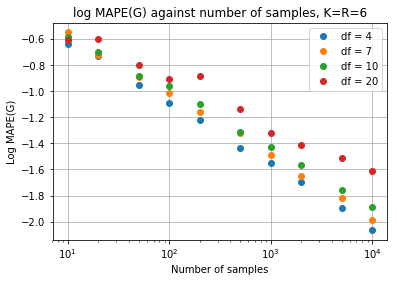
\includegraphics[width=0.45\textwidth]{Chap6_EvaluationAndAnalysis/distribution_variation/Convergence_DF_KR6_tdist_meanerr.png}
\end{subfigure}
\caption{Convergence plot for \(K=R=6\) models, when integrated using different values of the DOF \(\nu\). On the left is a plot of the MAPE, with \(95\%\) confidence intervals, the right without.}
\label{fig:ConvergencePlotTDOF}
\end{center}
\end{figure}

It was observed that varying \(\nu\) had a very similar effect to varying the covariance scale \(s\) in the case of the experiments Multivariate Gaussian sampling distribution. An increase in the value of \(\nu\) has a similar effect to decreasing the value of \(s\). As \(\nu\) is increased, the error distribution becomes more negatively biased and less symmetric, with heavier tails. This naturally makes the approximation \(\bar{M}\) more noisy. This is expected since the student-t sampling distribution approaches the Gaussian sampling distribution with scale \(s=1\), as \(\nu \rightarrow \infty\).

\begin{figure}[!htb]
\begin{center}
    \centering
    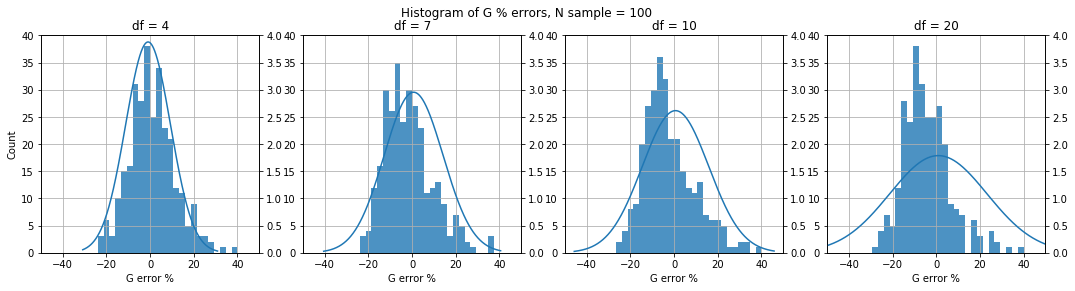
\includegraphics[width=1.0\textwidth]{Chap6_EvaluationAndAnalysis/distribution_variation/hist_KR6_tdist.png}
\caption{Error histograms of the errors vs. its Max Likelihood Gaussian for models where \(K=R=6\), and number of samples = \(100\), and different DOF values \(\nu\)}
\label{fig:hist_KR6_tdist}
\end{center}
\end{figure}

\begin{figure}[!htb]
\begin{center}
    \centering
    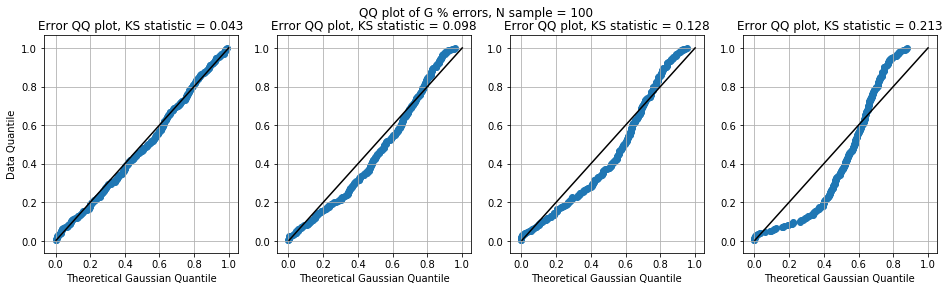
\includegraphics[width=1.0\textwidth]{Chap6_EvaluationAndAnalysis/distribution_variation/QQ_KR6_tdist.png}
\caption{QQ plot of the errors vs. its Max Likelihood Gaussian for models where \(K=R=6\), and number of samples = \(100\), and different DOF values \(\nu\)}
\label{fig:QQ_KR6_tdist}
\end{center}
\end{figure}

\begin{figure}[!htb]
\begin{center}
\begin{subfigure}
    \centering
    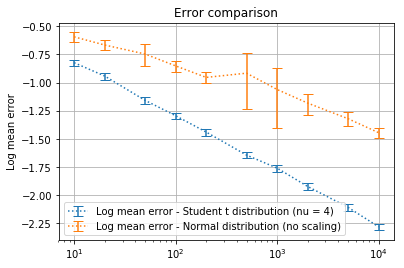
\includegraphics[width=0.45\textwidth]{Chap6_EvaluationAndAnalysis/distribution_variation/Convergence_KR6_tdist_vs_gaussian_s100.png}
\end{subfigure}
\begin{subfigure}
    \centering
    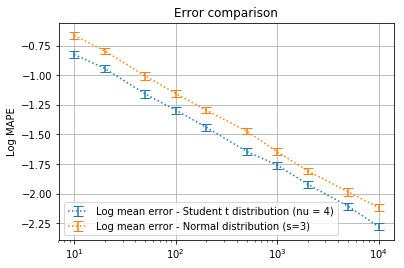
\includegraphics[width=0.45\textwidth]{Chap6_EvaluationAndAnalysis/distribution_variation/Convergence_KR6_tdist_vs_gaussian_s300.png}
\end{subfigure}
\caption{Convergence plot for \(K=R=6\) models. (Left) Comparison of student-t sampling distribution with \(\nu=4\) vs Gaussian sampling distribution with \(s=1\). (Right) Student-t with \(\nu=4\) vs Gaussian with \(s=3\)}
\label{fig:ConvergencePlotTvsGauss}
\end{center}
\end{figure}

A brief visualization of random logistic integrands overlaid with different sampling distributions can help aid understanding in why the sampling distributions play such an important part in reducing variance. Figure \ref{fig:distributiondistribution} shows \(100\) normalized (in both \(x\) and \(y\) axes) logistic integrand functions. The Student-t distribution with \(\nu=4\) and the Gaussian distribution with scale \(s=1\) is overlaid on the plot. The slower decay of the t-distribution away from the stationary point at the centre allows the t-distribution to be more robust in terms of its sampling of important regions in the integrand.
\\\\
As a final choice, the student-t distribution with a degree of freedom of \(\nu=4\) was chosen as the default sampling distribution. The choice for this was motivated by the fact that the t-distribution has some nice mathematical properties, such as a heavier tail that prevents unbounded weights during Monte Carlo sampling (details please refer to section \ref{sec:MCI}). The choice of \(\nu=4\) was supported by the fact that this was the best performing value. Shown below is the standard error comparison between the results from using the t-distribution vs Gaussian distributions.

\begin{figure}[!htb]
\begin{center}
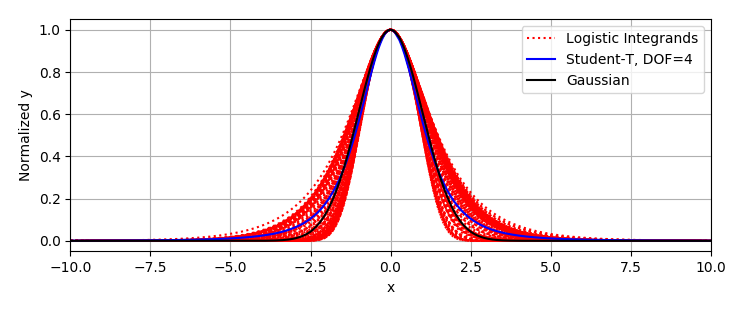
\includegraphics[width=1.\textwidth]{Chap6_EvaluationAndAnalysis/distribution_variation/dist_and_models.png}
\caption{ Randomly generated (2 station) models' logistic functions (normalized in x and y to have unit hessian and \(y=1\) at the stationary point), against a t-distribution (blue) and a Gaussian distribution (black).}
\label{fig:distributiondistribution}
\end{center}
\end{figure}

\subsection{Choice of Transform}

We next turn our attention to the effect of the choice of the logistic transformation on the error distribution. As before, experiments were conducted for the cases: \((K=R=2)\), \((K=R=4)\), and \((K=R=6)\). The conclusions from all 3 studies were very similar, and the version for \((K=R=6)\) is presented here. For plots and tables for the cases \((K=R=2)\), \((K=R=4)\), please refer to appendix \ref{app:extra_experiments}.
\\\\
Shown in table \ref{tab:NC_MAPE_transforms} are the tabulated MAPE (denoted \(\bar{M}(G)\)) and estimated \(95\%\) confidence intervals for the computed normalizing constant. The results for both additive and multiplicative transforms are considered. From a first look, there does not seem to be a significant difference between the two transformations. A more detailed look into the plots and t-distribution of the error prediction confirms this. \\
\begin{table}[!htb]
\begin{center}
    \begin{tabular}{@{}lllllll@{}}
    \toprule
     \(n_s\) & \multicolumn{3}{l}{Additive} & \multicolumn{3}{l}{Multiplicative} \\ \midrule
        & \(\bar{M}(G)\) \% & (-)\% & (+)\% & \(\bar{M}(G)\) \% & (-)\% & (+)\%  \\ \midrule
        10 &\(26.2\) & \(24.4\) & \(28.1\) & \(24.8\) & \(23.1\) & \(26.6\)  \\ 
        20 &\(18.9\) & \(17.8\) & \(20.1\) & \(18.2\) & \(17.2\) & \(19.3\)  \\ 
        50 &\(12.3\) & \(11.6\) & \(12.9\) & \(12\) & \(11.3\) & \(12.7\)  \\ 
        100 &\(8.7\) & \(8.24\) & \(9.16\) & \(8.3\) & \(7.88\) & \(8.71\)  \\ 
        200 &\(6.6\) & \(6.26\) & \(6.94\) & \(6.05\) & \(5.73\) & \(6.37\)  \\ 
        500 &\(4\) & \(3.81\) & \(4.2\) & \(3.75\) & \(3.56\) & \(3.94\)  \\ 
        1000 &\(3.07\) & \(2.93\) & \(3.21\) & \(2.71\) & \(2.57\) & \(2.84\)  \\ 
        2000 &\(2.09\) & \(1.99\) & \(2.19\) & \(1.94\) & \(1.84\) & \(2.04\)  \\ 
        5000 &\(1.22\) & \(1.16\) & \(1.28\) & \(1.18\) & \(1.12\) & \(1.24\)  \\ 
        10000 &\(0.89\) & \(0.846\) & \(0.934\) & \(0.866\) & \(0.821\) & \(0.911\)  \\    \bottomrule
    \end{tabular}
\end{center}
\caption{Normalizing constant MAPE \(M(G)\) \(95 \%\) confidence intervals for \(K=R=6\), for both transforms}
\label{tab:NC_MAPE_transforms}
\end{table}

We first observe the histograms and the quantile-quantile (QQ) plot in figure \ref{fig:ErrorHistAndQQPlot}, and confirm that the error distributions for both transforms are well approximated by a normal distribution.
\begin{figure}[!htb]
\begin{center}
\begin{subfigure}
    \centering
    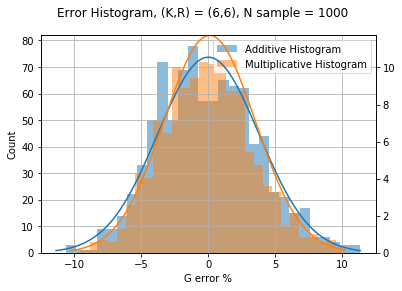
\includegraphics[width=0.45\textwidth]{Chap6_EvaluationAndAnalysis/transform_variation/hist_KR6_transforms.png}
\end{subfigure}
\begin{subfigure}
    \centering
    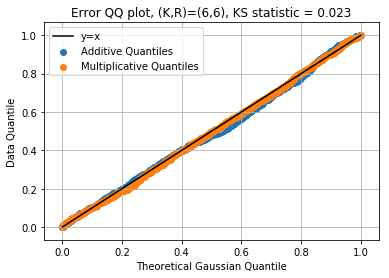
\includegraphics[width=0.45\textwidth]{Chap6_EvaluationAndAnalysis/transform_variation/QQ_KR6_transforms.png}
\end{subfigure}
\caption{(Left) Error distribution histogram and maximum likelihood gaussian. (Right) QQ plot of data quantiles vs. theoretical quantiles. \(N_{sample}=1000\)}
\label{fig:ErrorHistAndQQPlot}
\end{center}
\end{figure}

Plotting the estimated mean absolute error \(\bar{M}\) with its confidence intervals in figure \ref{fig:Convergence_Transforms}, it can be seen that the two transforms are quite similar in terms of errors.

\begin{figure}[!htb]
\begin{center}
\begin{subfigure}
    \centering
    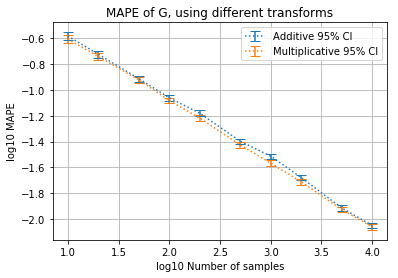
\includegraphics[width=0.45\textwidth]{Chap6_EvaluationAndAnalysis/transform_variation/Stderr_convergence_KR6_transforms.png}
\end{subfigure}
\begin{subfigure}
    \centering
    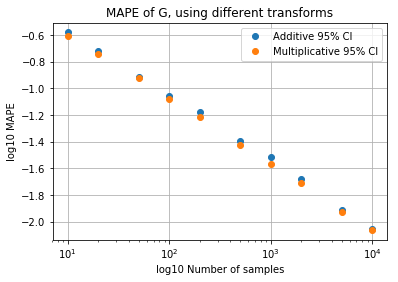
\includegraphics[width=0.45\textwidth]{Chap6_EvaluationAndAnalysis/transform_variation/MAPE_convergence_KR6_transforms.png}
\end{subfigure}
\caption{Convergence plots of MAPE and 95\% confidence intervals from the t-distribution of true MAPE \(M\) (Left), without errorbars (right) for different transforms. }
\label{fig:Convergence_Transforms}
\end{center}
\end{figure}

Figure \ref{fig:Posterior_sigma_transforms} shows the t-distribution estimating the distribution of the true MAPE \(M\). While the t-distributions for the true value of MAPE \(M\) for \(N=100\), \(N=1000\), and \(N=10000\) show a very slight tendency for the multiplicative transform to have a lower MAPE, no conclusive evidence can be drawn due to the large and frequent overlap of the confidence intervals.
\begin{figure}[!htb]
\begin{center}
\begin{subfigure}
    \centering
    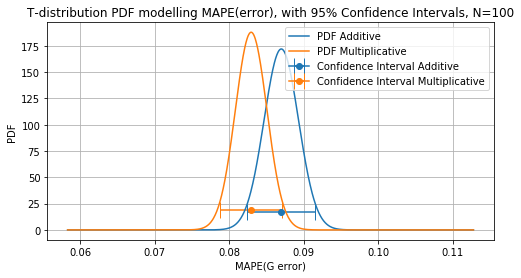
\includegraphics[width=0.45\textwidth]{Chap6_EvaluationAndAnalysis/transform_variation/poterior_KR6_transforms_N100.png}
\end{subfigure}
\begin{subfigure}
    \centering
    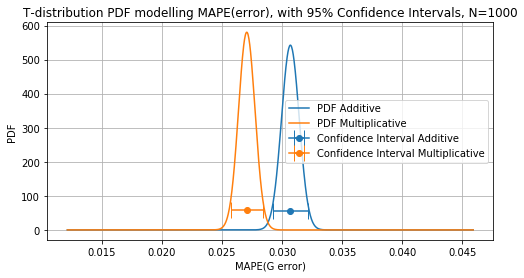
\includegraphics[width=0.45\textwidth]{Chap6_EvaluationAndAnalysis/transform_variation/poterior_KR6_transforms_N1000.png}
\end{subfigure}
\begin{subfigure}
    \centering
    \includegraphics[width=0.45\textwidth]{Chap6_EvaluationAndAnalysis/transform_variation/poterior_KR6_transforms_N10000.png}
\end{subfigure}
\caption{ T - distributions of the true MAPE, given the estimated MAPE \(\bar{M}\) for different transforms.}
\label{fig:Posterior_sigma_transforms}
\end{center}
\end{figure}

From the observed error distributions in this experiments, there is no conclusive evidence to support the fact that one transform has a consistently better performance than the other. 

\section{Introducing Delays}\label{sec:Analyze_Delays}

The introduction of delays into the evaluated model is of interest because it involves evaluating a different integral from from that of the single server case. See sections \ref{sec: multi_server_simplex_integral} and \ref{ssec:infinte_server_networks_results} for details. Table \ref{tab:convergence_tabulated_errors_SM_delay} and figure \ref{fig:OverallConvergence_Delay} shows the convergence behaviour of errors with increasing number of integration samples. This is very similar in terms of trend and magnitudes to that of the single-server case.\\

\begin{table}[!htb] 
\begin{center}
\begin{tabular}{@{}llll@{}}
\toprule
    \(N\) & KS score & \(\bar{M}(G)\)  & \(\hat{\sigma}(G)\) \\  \midrule
    10 &\(0.086\) & \(0.221\) & \(0.332\)  \\ 
    20 &\(0.048\) & \(0.156\) & \(0.206\)  \\ 
    50 &\(0.066\) & \(0.104\) & \(0.144\)  \\ 
    100 &\(0.054\) & \(0.075\) & \(0.100\)  \\ 
    200 &\(0.066\) & \(0.052\) & \(0.077\)  \\ 
    500 &\(0.055\) & \(0.034\) & \(0.046\)  \\ 
    1000 &\(0.056\) & \(0.023\) & \(0.032\)  \\ 
    2000 &\(0.048\) & \(0.017\) & \(0.023\)  \\ 
    5000 &\(0.057\) & \(0.011\) & \(0.014\)  \\ 
    10000 &\(0.033\) & \(0.007\) & \(0.010\)  \\      \bottomrule
\end{tabular}
\end{center}
\caption{Tabulated Mean Absolute Percentage Error, for small models \(K,R \in [2,4,6]\) with delay}
\label{tab:convergence_tabulated_errors_SM_delay}
\end{table} 

\begin{figure}[!htb]
\begin{center}
\begin{subfigure}
    \centering
    \includegraphics[width=0.45\textwidth]{Chap6_EvaluationAndAnalysis/images/OverallConvergence_Delay.png}
\end{subfigure}
\begin{subfigure}
    \centering
    \includegraphics[width=0.45\textwidth]{Chap6_EvaluationAndAnalysis/images/OverallConvergenceSigma_Delay.png}
\end{subfigure}
\caption{ Convergence plots for MAPE \(\bar{M}(G)\) (with 95\% CI's on the right) for small models with delay.}
\label{fig:OverallConvergence_Delay}
\end{center}
\end{figure}

\begin{figure}[!htb]
\begin{center}
\includegraphics[width=.9\textwidth]{Chap6_EvaluationAndAnalysis/images/ConvergenceNumberOfStations_SM_Delay.png}
\caption{Convergence plots for MAPE \(E(G)\) and standard error \(\sigma\) for small models with delay, separated by number of stations.}
\label{fig:ConvergenceNumberOfStations_SM_Delay}
\end{center}
\end{figure}

Models with delays behave similarly when the number of stations in the network increases. This is shown by the convergence plots in figure \ref{fig:ConvergenceNumberOfStations_SM_Delay}. Finally, comparing the single server only networks alongside the networks with delays, we see that the delay networks have a slightly higher MAPE and standard error. This can be attributed to the fact that an extra dimension is introduced to the integral.

\begin{figure}[!htb]
\begin{center}
\begin{subfigure}
    \centering
    \includegraphics[width=0.45\textwidth]{Chap6_EvaluationAndAnalysis/images/ConvergenceComparison_DelayNoDelay_meanerr.png}
\end{subfigure}
\begin{subfigure}
    \centering
    \includegraphics[width=0.45\textwidth]{Chap6_EvaluationAndAnalysis/images/ConvergenceComparison_DelayNoDelay.png}
\end{subfigure}
\caption{ Convergence plots for MAPE \(\bar{M}(G)\) and standard error \(\sigma\) for smalle models with and without delay.}
\label{fig:ConvergenceComparison_DelayNoDelay}
\end{center}
\end{figure}


\section{Multi-server Networks}\label{sec:Multiserver}

\subsection{Variance Cancellation}
In the case of multi-server networks, two approaches to computing the normalizing constant \(\mathbf{G}\) were employed. These were the summations first method, and the integrals first method, summarized in section \ref{sec:Multiserver}. The phenomenon of variance cancellation in the case of integrals first was explained, and in this section, selected experiments are run to demonstrate this phenomenon.
\\\\
In this experiment, a simple 2-station, single class model was considered. The population \(N\) was increased from \(1\) to \(12\). The demand matrix \(\boldsymbol{\theta}\) and the server vector \(\mathbf{s}\) was set as follows:
\[ \boldsymbol{\theta} = \left[ \begin{array}{cc}
0.8 \\
0.6
\end{array} \right]
%
\quad
\mathbf{s} = \left[ \begin{array}{cc}
2 \\
2
\end{array} \right]
\]
Since the normalizing constant is a difference of multiple integrals, we group the positive terms into \(G^{(+)}(\mathbf{x})\) and the negative terms into \(G^{(-)}(\mathbf{x})\):

\begin{equation}
\begin{split}
    G_\theta(\mathbf{N}) & = \frac{1}{\prod_{r=1}^R N_r!} \sum_{\mathbf{0 \leq v <s}} \mathbf{\alpha_v} \boldsymbol{\Delta}_{t_0}^{N-v} \boldsymbol{\Delta}_{\mathbf{t}}^{\mathbf{v}} I(N, t_0, \mathbf{t}) \\
    & = G_\theta^{(+)}(\mathbf{N}) + G_\theta^{(-)}(\mathbf{N})
\end{split}
\end{equation}

Each integral \(I(N, t_0, \mathbf{t})\) was evaluated with \(10^4\) samples. Each model was evaluated 30 times, where the mean value and the standard deviation of \(G_\theta(\mathbf{N})\), \(G_\theta^{(+)}(\mathbf{N})\), and \(G_\theta^{(-)}(\mathbf{N})\) was computed. The results are shown in table \ref{tab:Multiserver_var_cancel}.\\

\begin{table}[!htb] 
\begin{center}
\begin{tabular}{@{}lllllllll@{}}
\toprule
    \(N\) &\(G_{\theta,\text{EXACT}}\) & \(\mu(G^{(+)}_\theta)\) & \(\mu(G^{(-)}_\theta)\)  & \(\mu(G_\theta)\) & \(\sigma(G^{(+)}_\theta)\) & \(\sigma(G^{(-)}_\theta)\)  & \(\sigma(G_\theta)\) \\  \midrule
    1 & \(1.400e+0\) &\(1.400e+0\) & \(0.000e+3\) & \(1.400e+0\) & \(9.283e-4\) & \(0.000e+3\) & \(9.283e-4\) &  \\ 
    2 & \(9.800e-1\) &\(1.972e+0\) & \(-9.917e-1\) & \(9.801e-1\) & \(1.123e-3\) & \(3.937e-4\) & \(1.235e-3\) &  \\ 
    3 & \(5.180e-1\) &\(2.616e+0\) & \(-2.098e+0\) & \(5.181e-1\) & \(1.137e-3\) & \(7.548e-4\) & \(1.332e-3\) &  \\ 
    4 & \(2.450e-1\) &\(3.637e+0\) & \(-3.391e+0\) & \(2.447e-1\) & \(1.340e-3\) & \(1.660e-3\) & \(2.150e-3\) &  \\ 
    5 & \(1.093e-1\) &\(5.132e+0\) & \(-5.023e+0\) & \(1.091e-1\) & \(1.952e-3\) & \(1.725e-3\) & \(2.220e-3\) &  \\ 
    6 & \(4.713e-2\) &\(7.238e+0\) & \(-7.193e+0\) & \(4.854e-2\) & \(2.526e-3\) & \(3.158e-3\) & \(3.796e-3\) &  \\ 
    7 & \(1.987e-2\) &\(1.016e+1\) & \(-1.014e+1\) & \(2.061e-2\) & \(4.119e-3\) & \(3.515e-3\) & \(5.460e-3\) &  \\ 
    8 & \(8.256e-3\) &\(1.421e+1\) & \(-1.420e+1\) & \(9.953e-3\) & \(5.934e-3\) & \(5.881e-3\) & \(8.302e-3\) &  \\ 
    9 & \(3.394e-3\) &\(1.981e+1\) & \(-1.980e+1\) & \(3.656e-3\) & \(6.373e-3\) & \(7.972e-3\) & \(1.064e-2\) &  \\ 
    10 & \(1.385e-3\) &\(2.759e+1\) & \(-2.760e+1\) & \(-3.668e-3\) & \(9.180e-3\) & \(9.310e-3\) & \(1.240e-2\) &  \\ 
    11 & \(5.624e-4\) &\(3.841e+1\) & \(-3.843e+1\) & \(-1.768e-3\) & \(1.784e-2\) & \(1.322e-2\) & \(2.329e-2\) &  \\ 
    12 & \(2.274e-4\) &\(5.346e+1\) & \(-5.349e+1\) & \(-7.763e-3\) & \(2.171e-2\) & \(2.286e-2\) & \(2.850e-2\) &  \\ \bottomrule
\end{tabular}
\end{center}
\caption{Multiserver example variance cancellation}
\label{tab:Multiserver_var_cancel}
\end{table} 

As can be seen in table \ref{tab:Multiserver_var_cancel}, the value of the standard deviation of \(G_\theta\):  \[\sigma(G_\theta) \approx \sqrt{(\sigma(G_\theta^{(+)})^2 + \sigma(G_\theta^{(-)})^2} \]

With small \(N\), this is not a problem since \(\sigma(G_\theta) << G_\theta \approx G_{\theta, \text{EXACT}}\). At about \(N=7\) and \(N=8\), the values of \(G_{\theta}^{(+)}\) and \(G_{\theta}^{(-)}\) become quite large in magnitude, while their respective variances are kept small. However, the magnitude of their differences \(G_\theta\) becomes quite small relative to the standard deviations \(\sigma(G_{\theta}^{(+)})\) and \(\sigma(G_{\theta}^{(-)})\), this can be confirmed by looking at \(G_{\theta,\text{EXACT}}\). Past \(N=8\), the magnitude of the standard deviation is larger than that magnitude of \(G_{\theta,\text{EXACT}}\), and it becomes impossible to recover any information from the approximate solution of \(G_\theta\). 

\subsection{Testing with Fixed Models}

It was eventually agreed that the second method of the multiserver algorithm was to be used. This involves evaluating the following form of the multiserver normalizing constant:
\begin{equation*}
    G_\theta(\mathbf{N}) = \int_{\mathbb{R}^K} \bigg( \frac{1}{\prod_{r=1}^R N_r!} \sum_{\mathbf{0 \leq v <s}} \mathbf{\alpha_v} \boldsymbol{\Delta}_{t_0}^{N-v} \boldsymbol{\Delta}_{\mathbf{t}}^{\mathbf{v}} e^{-h(\mathbf x, t_0, \mathbf{t})}  \bigg) d \mathbf{x}
\end{equation*}

This decision is supported by the following experimental results. 
\\\\
The first test conducted was to perform the same calculations for the model that was used to highlight the variance cancellation phenomenon. The number of samples used was \(n_s=100\), over 2 order of magnitudes less than that used in method 1. For each population \(N\), 100 evaluations were made. The estimated MAPE \(\tilde{M}\), 95\% confidence intervals on the true MAPE \(M\), and the estimated standard error \(\hat{\sigma}_{ML}\) is shown in table \ref{tab:Multiserver_no_var_cancel}. \\

\begin{table}[!htb] 
\begin{center}
\begin{tabular}{@{}llllll@{}}
\toprule
    \(N\) & \(\bar{M} \%\) & \(\bar{M}\) \(95\%\) CI (+) & \(\bar{M}\) \(95\%\) CI (-) & \(\hat{\sigma}_{ML}\)\\ \midrule
    1 &\(0.808\) & \(0.692\) & \(0.924\) & \(0.994\) &  \\ 
    2 &\(0.883\) & \(0.742\) & \(1.02\) & \(1.13\) &  \\ 
    3 &\(0.942\) & \(0.809\) & \(1.08\) & \(1.15\) &  \\ 
    4 &\(0.824\) & \(0.706\) & \(0.943\) & \(1.02\) &  \\ 
    5 &\(0.891\) & \(0.744\) & \(1.04\) & \(1.13\) &  \\ 
    6 &\(0.829\) & \(0.707\) & \(0.952\) & \(1.03\) &  \\ 
    7 &\(0.856\) & \(0.725\) & \(0.986\) & \(1.07\) &  \\ 
    8 &\(0.882\) & \(0.749\) & \(1.01\) & \(1.1\) &  \\ 
    9 &\(0.808\) & \(0.685\) & \(0.93\) & \(1.02\) &  \\ 
    10 &\(1.01\) & \(0.855\) & \(1.17\) & \(1.27\) &  \\ 
    11 &\(1.25\) & \(1.08\) & \(1.42\) & \(1.5\) &  \\ 
    12 &\(1.12\) & \(0.939\) & \(1.31\) & \(1.46\) &  \\  \bottomrule
\end{tabular}
\end{center}
\caption{Multiserver example without variance cancellation}
\label{tab:Multiserver_no_var_cancel}
\end{table}

From table \ref{tab:Multiserver_no_var_cancel}, it can be clearly seen that the evaluated normalizing constants using the second method does not suffer from the same problem as was faced in the first, integrals first method.\\

In a second test, four hand-picked models were tested. We set the number of stations and classes to be \(K=R=2\). In a similar vein to the test with single-server nodes only, we select models which correspond to different loading shares on the stations. This is done by fixing the demand values for station \(0\) to \(1\):
\[\theta_{00} =\theta_{01} = 1\]

Besides that the population vector was fixed to \(\mathbf{N} = [3,3]\). The load shares were varied by changing the demands to station 1, \(\theta_{10}\) and \(\theta_{11}\), as well as the number of servers to stations \(0\) and \(1\), \([s_0, s_1]\). The definition of these models are shown in table \ref{tab:specific_models_evaluate_MS}. For each model, \(300\) evaluations were performed, and the estimated MAPE \(\tilde{M}\) and its confidence intervals were calculated. 
\\\\
The results are shown in table \ref{tab:specific_models_error_MS}. It can be seen that similarly defined models have similar MAPE estimates. The histogram and quantile-quantile plot for the errors for models \(4\) and model \(1\) are shown in figures \ref{fig:multiserver_d0_5s21} and \ref{fig:multiserver_d2s22} respectively. Good conformity with the normal distribution is also observed.

\begin{table}[!htb] 
\begin{center}
\begin{tabular}{@{}lllll@{}}
\toprule
 Test Case &  \([s_0, s_1]\) & \(\theta_{10}, \theta_{11}\) & Description \\ \midrule
 1 & \([2, 2]\) & \(2.0\) & Heavier load on station 1 \\
 2 & \([1, 2]\) & \(2.0\) & Perfectly equal loads\\
 3 & \([2, 2]\) & \(0.5\) & Heavier load on station 0 \\
 4 & \([2, 1]\) & \(0.5\) & Perfectly equal loads \\ \bottomrule
\end{tabular}
\end{center}
\caption{Models tested}
\label{tab:specific_models_evaluate_MS}
\end{table} 

\begin{table}[!htb] 
\begin{center}
\begin{tabular}{@{}llllll@{}}
\toprule
 Test Case & \(\bar{M} \%\) & \(\bar{M}\) \(95\%\) CI (+) & \(\bar{M}\) \(95\%\) CI (-) & \(\hat{\sigma}_{ML}\)\\ \midrule
    1 &\(1.28\) & \(1.17\) & \(1.38\) & \(1.59\) &  \\ 
    2 &\(0.777\) & \(0.71\) & \(0.844\) & \(0.974\) &  \\ 
    3 &\(1.4\) & \(1.27\) & \(1.53\) & \(1.81\) &  \\ 
    4 &\(0.767\) & \(0.703\) & \(0.831\) & \(0.94\) &  \\  \bottomrule
\end{tabular}
\end{center}
\caption{Model errors}
\label{tab:specific_models_error_MS}
\end{table}
 
\begin{figure}[!htb]
\begin{center}
\includegraphics[width=0.8\textwidth]{Chap6_EvaluationAndAnalysis/multiserver/d0_5s21.png}
\caption{ Histogram and QQ plot for model with \(\theta_{10} = \theta_{11} = 0.5\) and \([s_0, s_1] = [2,1]\)}
\label{fig:multiserver_d0_5s21}
\end{center}
\end{figure}

\begin{figure}[!htb]
\begin{center}
\includegraphics[width=0.8\textwidth]{Chap6_EvaluationAndAnalysis/multiserver/d2s22.png}
\caption{ Histogram and QQ plot for model with \(\theta_{10} = \theta_{11} = 0.5\) and \([s_0, s_1] = [2,2]\)}
\label{fig:multiserver_d2s22}\end{center}
\end{figure}

\subsection{Experimentation with Random Single Class Models}
To test the multi-server algorithm with larger models, the following test was carried out:
\begin{itemize}[noitemsep]
    \item Number of classes \(R\) was set to be one
    \item Number of stations was varied, \(K \in [2,4,6]\)
    \item Population \(N\) was chosen to be in \(\mathcal{U}(1,5)\).
    \item Demands were randomized.
    \item The Queue Lengths \(Q_{kr}\) and Throughputs \(\lambda_{r}\) were calculated using the Multiserver Logistic Sampling Algorithm.
    \item The exact queue lengths and throughputs were calculated using the exact MVA algorithm in JMVA. Only single classes are accomodated by the JMVA implementation, hence the restriction on \(R=1\).
\end{itemize}

To calculated the mean queue length per station, the following was used:
\begin{equation*}
    Q_{kr} = \sum_{n_r = 0}^{N_r} n_r P(n_{kr}=n_r | \mathbf{N});
\end{equation*}
Where the marginal probability \(P(n_{kr}=n_r | \mathbf{N})\) was calculated according to:
\begin{equation*}
    P(n_{kr}=n_r | \mathbf{N}) = \sum_{\substack{\mathbf{n}_k \\ n_{kr} = n_r}} F_{k}(\mathbf{n}_k) \frac{ G(-\mathbf{1}_k, \mathbf{N} - \mathbf{n}_k) }{ G(\mathbf{N}) }
\end{equation*}

Where:
\begin{equation*}
\begin{split}
    F_{k}(\mathbf{n}_k) = \frac{1}{\beta(n_k)} n_k! \prod_{r=1}^R \frac{\theta_{kr}^{n_kr}}{n_{kr}!} \\
    \beta(n_k) = \begin{cases} m_k! m_k^{n_k-m_k} & n_k > m_k \\ n_k! & n_k \leq m_k \end{cases}
\end{split}
\end{equation*}

The reported errors are as below:

\begin{table}[!htb] 
\begin{center}
\begin{tabular}{@{}llll@{}}
\toprule
    \(n_s\) & \(Q_{kr}\) MAPE \(\%\) & \(\lambda_r\) MAPE \(\%\) &  \\  \midrule
    10 &\(15.6\) & \(18.8\) &  \\ 
    20 &\(12.3\) & \(13.5\) &  \\ 
    50 &\(8.17\) & \(8.05\) &  \\ 
    100 &\(6.69\) & \(6.13\) &  \\ 
    200 &\(5.1\) & \(4.34\) &  \\ 
    500 &\(3.6\) & \(2.48\) &  \\ 
    1000 &\(3.11\) & \(1.68\) &  \\ 
    2000 &\(2.68\) & \(1.33\) &  \\ 
    5000 &\(2.26\) & \(0.764\) &  \\ 
    10000 &\(2.11\) & \(0.575\) &  \\  \bottomrule
\end{tabular}
\end{center}
\caption{Model errors}
\label{tab:convergence_error_MS}
\end{table}

And the resulting convergence plots are as shown in figure \ref{fig:Convergence_multiserver}.

\begin{figure}[!htb]
\begin{center}
\begin{subfigure}
    \centering
    \includegraphics[width=0.45\textwidth]{Chap6_EvaluationAndAnalysis/multiserver/convergence_MS.png}
\end{subfigure}
\begin{subfigure}
    \centering
    \includegraphics[width=0.45\textwidth]{Chap6_EvaluationAndAnalysis/multiserver/convergence_MS_meanerr.png}
\end{subfigure}
\caption{ Convergence plots for MAPE \(\bar{M}(Q_{kr})\), when compared to exact MVA}
\label{fig:Convergence_multiserver}
\end{center}
\end{figure}

The reason for the unusual trend in the queue length plot is due to the fact that the exact MVA solver reports the queue lengths in the wrong order under certain conditions, which is outside of the scope of this project to debug. Shown in figure \ref{fig:Histogram_multiserver} is the histogram for queue length errors when \(10^3\) and \(10^4\) samples are used. Highlighted are the errors for when the MVA solver reports the queue lengths in the wrong order. The vast majority of queue lengths reported have much lower errors.

\begin{figure}[!htb]
\begin{center}
\begin{subfigure}
    \centering
    \includegraphics[width=0.45\textwidth]{Chap6_EvaluationAndAnalysis/multiserver/histogram_QL_1000samples.png}
\end{subfigure}
\begin{subfigure}
    \centering
    \includegraphics[width=0.45\textwidth]{Chap6_EvaluationAndAnalysis/multiserver/histogram_QL_10000samples.png}
\end{subfigure}
\caption{ Histogram for QL errors (left) when \(10^3\) samples are used, (right) when \(10^4\) samples are used}
\label{fig:Histogram_multiserver}
\end{center}
\end{figure}

\subsection{Experimentation with Random MultiClass Models}
To test the multi-server algorithm with multiclass models, the following test was carried out:
\begin{itemize}[noitemsep]
    \item Number of classes \(R\) was set to be in \([1,2]\)
    \item Number of stations was varied, \(K \in [2,3]\)
    \item Population \(\mathbf{N}\) was chosen to be in \(\mathcal{U}(1,5)\).
    \item Demands were randomized.
    \item The Normalizing Constant \(G_{\boldsymbol{\theta}(\mathbf{N})}\) calculated using the Multiserver Logistic Sampling Algorithm.
    \item The exact answer is calculated using a MATLAB implementation of a recursive algorithm for \(G_{\boldsymbol{\theta}(\mathbf{N})}\) - \texttt{pfqn\_gmvald()}.
\end{itemize}

The model size hyperparameters \(K\), \(R\) and \(N\) were chosen such that the computation times for exact MVA stayed within reasonable limits. The convergence plot is shown in figure \ref{fig:Convergence_NC_multiserver}.

\begin{figure}[!htb]
\begin{center}
\begin{subfigure}
    \centering
    \includegraphics[width=0.45\textwidth]{Chap6_EvaluationAndAnalysis/multiserver/convergence_NC_MS.png}
\end{subfigure}
\begin{subfigure}
    \centering
    \includegraphics[width=0.45\textwidth]{Chap6_EvaluationAndAnalysis/multiserver/convergence_NC_MS_meanerr.png}
\end{subfigure}
\caption{ Convergence plots for MAPE \(\bar{M}(Q_{kr})\), when compared to exact MVA}
\label{fig:Convergence_NC_multiserver}
\end{center}
\end{figure}

The effect of station number on the accuracy is also very similar to the single-server only network case.

\begin{figure}[!htb]
\begin{center}
\includegraphics[width=\textwidth]{Chap6_EvaluationAndAnalysis/multiserver/convergence_NC_MS_meanerr_class_separated.png}
\caption{ Convergence plots for MAPE \(\bar{M}(G)\), when compared to exact MVA}
\label{fig:Convergence_NC_multiserver_class_separated}
\end{center}
\end{figure}

\begin{table}[!htb] 
\begin{center}
\begin{tabular}{@{}lllll@{}}
\toprule
    \(n_s\) & \(95\% (+)\) \(\%\) & \(95\% (-)\) \(\%\) & \(\bar{M} \%\) &  \\  \midrule
    10 &\(7.47\) & \(6.27\) & \(6.87\) &  \\ 
    20 &\(5.26\) & \(4.28\) & \(4.77\) &  \\ 
    50 &\(3.23\) & \(2.69\) & \(2.96\) &  \\ 
    100 &\(2.25\) & \(1.87\) & \(2.06\) &  \\ 
    200 &\(1.7\) & \(1.4\) & \(1.55\) &  \\ 
    500 &\(0.972\) & \(0.801\) & \(0.886\) &  \\ 
    1000 &\(0.727\) & \(0.601\) & \(0.664\) &  \\ 
    2000 &\(0.543\) & \(0.445\) & \(0.494\) &  \\ 
    5000 &\(0.333\) & \(0.277\) & \(0.305\) &  \\ 
    10000 &\(0.244\) & \(0.203\) & \(0.224\) &  \\  \bottomrule
\end{tabular}
\end{center}
\caption{Tabulated MAPE for the computation of the normalizing constant, with \(95\%\) confidence intervals}
\label{tab:convergence_error_MS_NC}
\end{table}


\subsection{A few notes on large models}
It was observed that under larger models (large \(K\), \(R\) or \(N\)), the stationary point search can yield failure. This is due to insufficient precision in the calculation of the integrand, resulting in incorrect integrand values. The solver now takes in a \texttt{precision} argument, which dictates the precision (number of bits) the \texttt{BigDecimal} operations in the Logistic Sampling Algorithm uses. A value of \(128\) is sufficient for most small models, otherwise a value of \(256\) can accomodate many large models of interest (eg. \(K,R = 4, N=30 \)).

%%%%%%%%%%%%%%%%%%%%%%%%%%%%%%%%%%%%
\chapter{Conclusion}

We conclude the report with this chapter. In this chapter, the main project outcomes are summarized. These will be considered in terms of theoretical achievements, implementation of the software tools, as well as accuracy and speed of the algorithm. Areas for further, and more immediate work are also identified. Possible extensions are suggested which could potentially improve the efficiency of the algorithm.

\section{Summary of Project Outcomes}
\subsection{Theory}
\begin{itemize}[leftmargin=*]
    \item This report consolidates the required theory which forms the basis of the Logistic Sampling algorithm. It suggests alternative proofs to results first derived in \cite{Casale2017AcceleratingMethods}, to give integrals of the form:
    \[\int_{\Delta_K} f(\mathbf{u}) d \mathbf{u}\]
    \item Monte Carlo integration theory was succesfully applied to the analysis and improvement of the existing Logistic Sampling algorithm. A better sampling distribution - the student-t was parametrized and applied to the algorithm.
    \item Novel results for the logistic sampling algorithm utilizing the multiplicative logistic transform were derived, to give an alternative form of the logistic sampling algorithm in a different coordinate system. Theorems relating the logistic integrand function under the additive transform and multiplicative transforms were derived.
    \item The multi-server extension to the integral form of the normalizing constant was analyzed, and approaches to compute the integral suggested. New mathematical results, including stationary point equations and closed-form stationary point hessian expressions were derived.
    \item The variance cancellation phenomenon for the Logistic Sampling algorithm for multi-server networks was identified and proven to be true in numerical experiments.
\end{itemize}

\subsection{Software Implementation}
\begin{itemize}[leftmargin=*]
    \item Five versions of the Logistic Sampling Algorithm was implemented. Three logistic algorithms were implemented for the simplex integral form of the normalizing constant under the additive transform. This includes the single-server only case, single-server with delay, and multi-server networks. For functions under the multiplicative transform, only the first two were implemented and tested.
    \item The implementation of these algorithms was interfaced with the JMT front-end, to extend the suite of tools offered by JMVA. These are now available as an alternative performance measure algorithm in JMT.
    \item Modular and re-usable design of classes within the implementation makes it easy to improve upon, and extend the algorithm in software.
    \item Thorough testing and verification of the classes used in the final algorithm was performed through the strategy of unit testing. This report also provides documentation for the implemented classes.
\end{itemize}

\subsection{Evaluation of Algorithm}
\begin{itemize}[leftmargin=*]
    \item Thorough numerical experimentation of the Logistic Sampling algorithm was carried out. The results are thoroughly documented.
    \item A statistical framework and tools were established to analyze the distribution of errors of the Logistic Sampling algorithm. This included the use of t-distribution estimate of the true MAPE given an estimated value of the MAPE.
    \item Trends in the results were explained by alluding to Monte Carlo integration theory. The validity of Monte Carlo integration theory gives a good prediction tool of potential errors of the results of the Logistic Sampling algorithm.
    \item MAPE approximates were measured and tabulated to give users of the algorithm an expected accuracy of their results.
    \item The hypothesis that one form of transform was better than the other (among the additive and multiplicative transforms) was disproved by examining MAPE confidence intervals.
    \item The phenomenon of variance cancellation was established to be true through numerical experiments. The summations first method of the Logistic Sampling Algorithm was shown to be superior.
\end{itemize}

\section{Future Work}
\begin{itemize}[leftmargin=*]
    \item Immediate future work should focus on debugging and understanding the implementation of the multi-server algorithm. Numerical instability in the stationary point gradient descent is still preventing the algorithm from being able to accomodate larger models.
    \item Another area of further work would be to find an iterative set of equations for the multi-server stationary points, and remove the need for gradient descent. This will involve the solution of an equation of the form :
    \[-e^{k(\mathbf{x})} \sum_{\mathbf{0 \leq v <s}} \mathbf{\alpha_v} \boldsymbol{\Delta}_{t_0}^{N-v} \boldsymbol{\Delta}_{\mathbf{t}}^{\mathbf{v}} 
    \bigg[ -\frac{\partial}{\partial \mathbf{x}} \bigg(h(\mathbf{x}, t_0, \mathbf{t}) \bigg) e^{-h(\mathbf{x}, t_0, \mathbf{t})} \bigg] = \mathbf{0}\]
    \item The sampling efficiency could be improved by using higher order derivatives to parametrize an asymmetric sampling distribution that can achieve better variance reduction.
    \item Alternative transforms from the simplex to the real domain could be investigated and perhaps implemented for the Logistic Sampling algorithm. This could include the isometric log-ratio transformation, and centred log-ratio transformation \cite{Egozcue2003IsometricAnalysis}.
\end{itemize}


%% bibliography
\bibliographystyle{abbrv}
\bibliography{bibliography}

\begin{appendices}
    \chapter{Experimental Results}\label{app:extra_experiments}

\section{Additive vs. Multiplicative Transforms for \(K=R=2\)}

\begin{table}[H]
\begin{center}
    \begin{tabular}{@{}lllllll@{}}
    \toprule
     \(n_s\) & \multicolumn{3}{l}{Additive} & \multicolumn{3}{l}{Multiplicative} \\ \midrule
        & \(\bar{M}(G)\) \% & (-)\% & (+)\% & \(\bar{M}(G)\) \% & (-)\% & (+)\%  \\ \midrule
        10 &\(4.76\) & \(4.46\) & \(5.05\) & \(4.64\) & \(4.32\) & \(4.96\) \\ 
        20 &\(3.55\) & \(3.33\) & \(3.77\) & \(3.36\) & \(3.15\) & \(3.58\) \\ 
        50 &\(2.23\) & \(2.09\) & \(2.37\) & \(2.24\) & \(2.09\) & \(2.38\) \\ 
        100 &\(1.52\) & \(1.43\) & \(1.6\) & \(1.5\) & \(1.41\) & \(1.59\) \\ 
        200 &\(1.06\) & \(0.991\) & \(1.12\) & \(1.07\) & \(1.01\) & \(1.14\) \\ 
        500 &\(0.646\) & \(0.608\) & \(0.684\) & \(0.681\) & \(0.637\) & \(0.725\) \\ 
        1000 &\(0.486\) & \(0.456\) & \(0.516\) & \(0.476\) & \(0.445\) & \(0.506\) \\ 
        2000 &\(0.335\) & \(0.315\) & \(0.356\) & \(0.336\) & \(0.316\) & \(0.357\) \\ 
        5000 &\(0.208\) & \(0.195\) & \(0.22\) & \(0.206\) & \(0.193\) & \(0.218\) \\ 
        10000 &\(0.14\) & \(0.132\) & \(0.149\) & \(0.15\) & \(0.141\) & \(0.16\) \\   \bottomrule
    \end{tabular}
\end{center}
\caption{Normalizing constant MAPE \(M(G)\) and and 95\(\%\) confidence intervals for \(K=R=2\)}
\label{tab:NC_MAPE_transforms_KR2}
\end{table}

\newpage

\begin{figure}[H]
\begin{center}
    \includegraphics[width=0.6\textwidth]{figures/convergence_KR2.png}
\caption{Convergence plots of standard error and 95\% confidence intervals for the MAPE for different transforms. \(K=R=2\)}
\label{fig:Convergence_Transforms_KR2}
\end{center}
\end{figure}

\begin{figure}[H]
\begin{center}
\begin{subfigure}
    \centering
    \includegraphics[width=0.5\textwidth]{figures/KR2N100_post.png}
\end{subfigure}
\begin{subfigure}
    \centering
    \includegraphics[width=0.5\textwidth]{figures/KR2N1000_post.png}
\end{subfigure}
\begin{subfigure}
    \centering
    \includegraphics[width=0.5\textwidth]{figures/KR2N10000_post.png}
\end{subfigure}
\caption{ T - distributions of the true MAPE, given the estimated MAPE \(\bar{M}\) for different transforms. \(K=R=2\)}
\label{fig:Posterior_sigma_transforms_KR2}
\end{center}
\end{figure}

\newpage

\section{Additive vs. Multiplicative Transforms for \(K=R=4\)}

\begin{table}[H]
\begin{center}
    \begin{tabular}{@{}lllllll@{}}
    \toprule
     \(n_s\) & \multicolumn{3}{l}{Additive} & \multicolumn{3}{l}{Multiplicative} \\ \midrule
        & \(\bar{M}(G)\) \% & (-)\% & (+)\% & \(\bar{M}(G)\) \% & (-)\% & (+)\%  \\ \midrule
        10 &\(15.6\) & \(14.8\) & \(16.5\) & \(14.2\) & \(13.5\) & \(15\)  \\ 
        20 &\(11.9\) & \(11.2\) & \(12.5\) & \(10.2\) & \(9.62\) & \(10.7\)  \\ 
        50 &\(7.41\) & \(7.02\) & \(7.8\) & \(6.8\) & \(6.45\) & \(7.15\)  \\ 
        100 &\(5.2\) & \(4.95\) & \(5.45\) & \(4.71\) & \(4.47\) & \(4.94\)  \\ 
        200 &\(3.75\) & \(3.56\) & \(3.93\) & \(3.15\) & \(2.99\) & \(3.31\)  \\ 
        500 &\(2.32\) & \(2.2\) & \(2.44\) & \(2.08\) & \(1.98\) & \(2.18\)  \\ 
        1000 &\(1.66\) & \(1.58\) & \(1.74\) & \(1.5\) & \(1.42\) & \(1.58\)  \\ 
        2000 &\(1.22\) & \(1.15\) & \(1.28\) & \(1.03\) & \(0.976\) & \(1.08\)  \\ 
        5000 &\(0.734\) & \(0.696\) & \(0.772\) & \(0.641\) & \(0.609\) & \(0.672\)  \\ 
        10000 &\(0.518\) & \(0.492\) & \(0.544\) & \(0.478\) & \(0.453\) & \(0.502\)  \\   \bottomrule
    \end{tabular}
\end{center}
\caption{Normalizing constant MAPE \(M(G)\) and and 95\(\%\) confidence intervals for \(K=R=4\)}
\label{tab:NC_MAPE_transforms_KR4}
\end{table}


\begin{figure}[H]
\begin{center}
    \includegraphics[width=0.6\textwidth]{figures/convergence_KR4.png}
\caption{Convergence plots of standard error and 95\% confidence intervals for the MAPE for different transforms. \(K=R=4\)}
\label{fig:Convergence_Transforms_KR4}
\end{center}
\end{figure}

\newpage

\begin{figure}[H]
\begin{center}
\begin{subfigure}
    \centering
    \includegraphics[width=0.5\textwidth]{figures/KR4N100_post.png}
\end{subfigure}
\begin{subfigure}
    \centering
    \includegraphics[width=0.5\textwidth]{figures/KR4N1000_post.png}
\end{subfigure}
\begin{subfigure}
    \centering
    \includegraphics[width=0.5\textwidth]{figures/KR4N10000_post.png}
\end{subfigure}
\caption{ T - distributions of the true MAPE, given the estimated MAPE \(\bar{M}\) for different transforms. \(K=R=4\)}
\label{fig:Posterior_sigma_transforms_KR4}
\end{center}
\end{figure}

\newpage

\chapter{Usage Guide}
\section{Short guide for developers}

\begin{figure}[H]
\centering
\includegraphics[width=1.\textwidth]{figures/DevGuideUML.png}
\caption{ UML for SolverMulti Interface}
\label{fig:DevGuideUML}
\end{figure}

The Logistic Sampling algorithm is available for use through the \texttt{SolverMultiClosedMCL} class which implements the abstract class \texttt{SolverMulti}. This relationship is summarized in figure \ref{fig:DevGuideUML} The steps to use are as follows:

\begin{itemize}[noitemsep]
    \item Instantiate a \texttt{SolverMultiClosedMCL} object by calling its constructor: \texttt{SolverMultiClosedMCL(int classes, int stations, int[] population, int max\_samples, int precision)}
    \item Call \texttt{input(int[] t, double[][][]s, double[][] v)} to specify the model
    \item Call \texttt{solve()} to calculate the various performance metrics.
    \item The performance metrics are available throught the various getter methods declared in \texttt{SolverMulti}.
\end{itemize}

The constructor, \texttt{input()}, and \texttt{solve()} methods are described in table \ref{table:descriptions_of_methods}.

\begin{table}[H]
\centering
\begin{tabularx}{\textwidth}{@{}lXX@{}}
\toprule
Method  & Description \\ \midrule
Constructor   & Number of \texttt{classes} and \texttt{stations} are specified as \texttt{ints}, and \texttt{population} is specified as an array of \texttt{ints}. Number of samples to integrate over is specified in the fourth argument \texttt{max\_samples}. \texttt{precision} is the number of (base 10) digits that are used in the \texttt{BigDecimal} operations within the solver.\\\\
\texttt{input} & To specify the model, the types of the model are specified through an array of ints: \texttt{int[] t}. These can be \texttt{0} (LD), \texttt{1} (LI), and \texttt{2} (DELAY). For \texttt{LD} models, only multiserver types are supported. \newline \newline
For service times, this is represented through the second argument \texttt{double[][][] s}, where the first two dimensions of this 3-dimensional array is of length \texttt{classes} and \texttt{stations}. For \texttt{LI} and \text{DELAY} stations, the 3rd dimension is of length 1, for \texttt{LD} stations, the 3rd dimension is of length \texttt{population[r]} where \texttt{r} is the class referred to by that entry of the demand matrix. Furthermore, since the solver can only handle multi-server cases, the format of \texttt{double[][][] s} must be the following: 
\begin{equation*}
    \texttt{s[k][r][n]} = s_{kr} * \min(m,n)
\end{equation*}
Where \(s_{kr}\) is the service time associated with a single server in that station, and \(m\) is the number of servers of the station, and \(n\) is the class population considered. The above input must be correct up to 3 decimal places, and the solver will attempt to infer the value of  \(s_{kr}\) and \(m\), and print the server count on the screen.
\\\\
\texttt{solve()}  & When called, instantiates a \texttt{MonteCarloLogisticSolver} which will calculate the stationary point and its hessian of the logistic integrand. Then it will perform Monte Carlo integration over the specified logistic function, and store the values of the performance metrics. \\ \bottomrule
\end{tabularx}
\caption{Descriptions of methods}
\label{table:descriptions_of_methods}
\end{table}

\newpage

\section{Short guide for GUI users}

To use the Logistic Sampling Algorithm, selected \texttt{Logistic Sampling} from the drop down menu:
\begin{figure}[H]
\centering
\includegraphics[width=1.\textwidth]{figures/LogisticSampling_GUI_selection.png}
\caption{ Solver Selection Menu }
\label{fig:LogisticSampling_GUI_selection}
\end{figure}

The Logistic Sampling Solver hypter-parameters have to be specified. \texttt{Max Samples} represent the number of samples for which the Monte Carlo Integration will be carried out with. \texttt{Precision} represents the number of (base 10) digits which the \texttt{BigDecimal} operations will use in the algorithm.

\begin{figure}[H]
\centering
\includegraphics[width=1.\textwidth]{figures/LogisticSampling_GUI_hyperparams.png}
\caption{ Solver hyper-parameter specification }
\label{fig:LogisticSampling_GUI_hyperparams}
\end{figure}

To specify service times, one can enter a single number for \texttt{Load Independent} or \texttt{Delay} servers. For \texttt{Load Dependent} servers, the entries must be of the format:
\begin{equation*}
    \texttt{s[k][r][n]} = s_{kr} * \min(m,n)
\end{equation*}
Where \texttt{s[k][r][n} is the load-dependent service time for station \(k\), class \(r\), and for population \texttt{n}. \(s_{kr}\) is the service time associated with a single server in that station. \(m\) is the number of servers in that station. This number must be specified correctly to 3 decimal places. The solver will then attempt to infer the values of \(m\) and \(s_{kr}\) and display it to the console as confirmation.
\\\\
Shown below is the service time inputs for \textit{single-class 3-station model} with the following definitions for the 3 stations. Population for class 0 is \(4\):
\begin{itemize}[noitemsep]
    \item \textbf{Station 0}: Load independent with service time \(s_{00} = 2\)
    \item \textbf{Station 1}: Delay with service time \(s_{10} = 3\)
    \item \textbf{Station 2}: Multiserver with service time \(s_{20} = 8\) and \(m = 3\).
\end{itemize}

\begin{figure}[H]
\centering
\includegraphics[width=1.\textwidth]{figures/LogisticSampling_GUI_input.png}
\caption{ Solver input }
\label{fig:LogisticSampling_GUI_input}
\end{figure}

\newpage

\chapter{LSEPI Ethics Checklist}
\section{Discussion of Ethics in the Project}

The option 'yes' was checked for the following points in section 8 of the checklist (dual use):
\begin{itemize}
    \item Does your project have the potential for military applications?
    \item Does your project have an exclusive civilian application focus?
\end{itemize}

The aim of this project was for the research and optimization of civilian computer systems. However, it is possible that such tools can be used in a military context. Analytical modelling of computer systems, which is the primary function of software developed in this project, has a purely constructive role: to be able to model and predict performance of complex computer systems. However, it is also possible that such modelling tools be used as weapons to aid coordinated cyber-attacks. Being able to model and predict computer systems accurately , may be used in a military context to target vulnerable systems. However, this requires intimate knowledge of the system that is targeted, and it has never been used in such a context.
\\\\
In conclusion, while there may be a possibility of military use for the research software tools developed in this project, it is extremely unlikely that it would be used. There are no other major ethical concerns besides the one outlined above.

\newpage

\section{LSEPI Ethics Checklist}

\begin{figure}[H]
\begin{center}
\includegraphics[width=\textwidth]{Chapter8_Ethics/ethhics_p1.png}
\label{fig:ethics_p1}
\end{center}
\end{figure}

\newpage

\begin{figure}[H]
\begin{center}
\includegraphics[width=\textwidth]{Chapter8_Ethics/ethhics_p2.png}
\label{fig:ethics_p2}
\end{center}
\end{figure}
\end{appendices}

\end{document}
